\documentclass[a4print,english,lof,lot]{univpmphdthesis}
\errorcontextlines=9

\RequirePackage[utf8]{inputenc}
\RequirePackage[T1]{fontenc}

\usepackage{lmodern}
\usepackage[cmex10]{amsmath}
\usepackage{amssymb}
\usepackage{subcaption}
\usepackage{multirow}
\usepackage{booktabs}
\usepackage{framed}
\usepackage{algorithm,algpseudocode}
\usepackage[table,xcdraw]{xcolor}
\usepackage{pgfplots,pgfplotstable}
\usetikzlibrary{pgfplots.groupplots}
\usepackage{tabularx}

\usepackage{tikz}
\usetikzlibrary{shapes,arrows}

\usepackage{tkz-kiviat,numprint}
\usetikzlibrary{decorations.pathreplacing, arrows, fit}
\usepackage{hyperref}
\usepackage{lineno}

\usepackage{collcell}
\usepackage{hhline}
\usepackage{tablefootnote}
\usepackage{siunitx}
\usepackage{cleveref}
\usepackage{steinmetz}
\usepackage{url}


\usetikzlibrary{shadows,arrows,fit,shapes,positioning,calc,backgrounds,spy,decorations.markings}
\usetikzlibrary{backgrounds}

\pgfdeclarelayer{background}
\pgfdeclarelayer{foreground}
\pgfsetlayers{background,main,foreground}

\tikzstyle{bk} = [draw, fill=blue!30, text centered, minimum height=2em, text width=7em, minimum width=6em, minimum height=3em, rounded corners, drop shadow]
\tikzstyle{bkFull} = [draw, fill=blue!30, text centered, minimum height=2em, text width=15em, minimum width=20em, minimum height=3em, rounded corners, drop shadow]
\tikzstyle{bkDec} = [draw, fill=red!40, text centered, minimum height=2em, text width=15em, minimum width=15em, minimum height=3em, rounded corners, drop shadow]
\tikzstyle{cy} = [draw, fill=gray!30, text centered, minimum height=3em, text width=7em, minimum width=2em, cylinder, shape border rotate=90, shape aspect=0.1, drop shadow]
\tikzstyle{cyFull} = [draw, fill=gray!30, text centered, minimum height=3em, text width=7em, minimum width=20em, cylinder, shape border rotate=90, shape aspect=0.1, drop shadow, dashed]
\tikzstyle{bg}=[rectangle,fill=gray!30,inner sep=0.2cm,rounded corners,draw=black!50, dashed]
\tikzstyle{input} = [coordinate]

\tikzset{
	myarrow/.style={
		draw,thick,
		single arrow,
		%text width=1cm,
		minimum height=1cm,
		%anchor=west,
		%fill=white
	},
}

\tikzstyle{vecArrow} = [thick, decoration={markings,mark=at position 1 with {\arrow[semithick]{open triangle 60}}},
double distance=1.4pt, shorten >= 5.5pt, preaction = {decorate}, postaction = {draw,line width=1.4pt, white,shorten >= 4.5pt}]

\tikzstyle{innerWhite} = [semithick, white,line width=1.6pt, shorten >= 4.5pt]




\newcommand{\LegendBox}[3][]{%
	\xdef\fitbox{}%
	\coordinate[#1] (LegendBox_anchor) at (#2) ;
	\foreach \col/\item [count=\hi from 0] in {#3} {
		\node[color = \col,draw,thick,
		fill  = \col,
		minimum width  = 5 ex,
		minimum height = 1 ex,
		name=b\hi,
		] at ([yshift=0 ex,xshift=\hi*40 ex]LegendBox_anchor) {};
		\node[anchor=west,xshift=0.1 ex] at (b\hi.east) (c\hi) {\item};
		\xdef\fitbox{\fitbox(c\hi)}
	}%
	\node [fit=\fitbox(LegendBox_anchor), minimum width = 0 ex] {};
}


\newcommand{\chref}[1]{Chapter~\ref{#1}}
\newcommand{\secref}[1]{Section~\ref{#1}}
\newcommand{\subsecref}[1]{Subsection~\ref{#1}}
\newcommand{\paragref}[1]{Paragraph~\ref{#1}}

\newcommand{\apxref}[1]{Appendix~\ref{#1}}

\newcommand{\figref}[1]{\figurename~\ref{#1}}
\newcommand{\tableref}[1]{Table~\ref{#1}}
%\newcommand{\eqref}[1]{Equation~\ref{#1}}
\newcommand{\equationref}[1]{Eq.~\ref{#1}}

\newcommand*\rfrac[2]{{}^{#1}\!/_{#2}}


\def\N{{\mathbb{N}}}
\def\Z{{\mathbb{Z}}}
\def\R{{\mathbb{R}}}

\newcommand\norm[1]{\left\lVert#1\right\rVert}
% Il codice che segue colora una cella in base al suo contenuto
% #1 è il contenuto della cella (ad esempio, 80)
% \pgfmathparse{#1/100<.7?1:0} 

\newcommand\gray{gray}
\newcommand\ColCell[1]{%
	\pgfmathparse{#1/100<.7?1:0}% valuta se #1/100 è maggiore di 0.7 oppure è minore. Se minore ritorna 1, altrimenti 0
	\ifnum\pgfmathresult=0\relax\color{white}\fi % imposta il colore del testo a bianco se il risultato di pgfmathparse è 0
	\pgfmathparse{1-#1/100}% calcola 1-#1/100
	\expandafter\cellcolor\expandafter[%
	\expandafter\gray\expandafter]\expandafter{\pgfmathresult}#1} % colora la cella della gradazione di grigio impostata dal risultato di pgfmathparse ed inserisce il valore originario della cella.
\newcolumntype{E}{>{\collectcell\ColCell}c<{\endcollectcell}}
\newcolumntype{K}[1]{>{\centering\arraybackslash}p{#1}}
\newcolumntype{L}[1]{>{\raggedright\arraybackslash}p{#1}}
\newcolumntype{C}[1]{>{\centering\arraybackslash}p{#1}}
\newcolumntype{R}[1]{>{\raggedleft\arraybackslash}p{#1}}
%\modulolinenumbers[5]

%%%%%%%%%%%%%%%%%%%%%%%%%%%%%%%%%%%%%%%%%%%%%%%%%%%%%%%%%%%
% Metadata
%%%%%%%%%%%%%%%%%%%%%%%%%%%%%%%%%%%%%%%%%%%%%%%%%%%%%%%%%%%
\phdschool{Scuola di Dottorato di Ricerca in Scienze dell'Ingegneria}
\phdfaculty{Facolt\`{a} di Ingegneria}
\phdcurriculum{Curriculum in Ingegneria Elettronica, Elettrotecnica e delle Telecomunicazioni}
\phdtitle{Ambient Intelligence: Computational Audio Processing For Human Fall Detection}
%\phdsubtitle{con questa bellissima classe} % NON NECESSARIO
\phdauthor{Diego Droghini}
\phdadvisor{Prof.~Francesco Piazza}
\phdcoadvisor{Prof.~Stefano Squartini}
%\phdcoadvisor{Prof.~Michele Blu} % IN TEORIA NON E' AMMESSO
%\phdcurriculumadvisor{Prof.~Francesco Piazza}
\phdcycle{17}
%\thesisdedication{alla mia famiglia}
\phdlocation{Ancona}
\phdtime{Ottobre 2018}
%%%%%%%%%%%%%%%%%%%%%%%%%%%%%%%%%%%%%%%%%%%%%%%%%%%%%%%%%%%

% Solo per generare testo...
\usepackage{lipsum}

\begin{document}

%%%%%%%%%%%%%%%%%%%%%%%%%%%%%%%%%%%%%%%%%%%%%%%%%%%%%%%%%%%
% Front matter contents
%%%%%%%%%%%%%%%%%%%%%%%%%%%%%%%%%%%%%%%%%%%%%%%%%%%%%%%%%%%
\frontmatter

\maketitle

%\begin{thesisacknowledge}
%\lipsum[1-2]
%\end{thesisacknowledge}

%\begin{thesisacknowledge}[italian]
%\lipsum[1-2]
%\end{thesisacknowledge}

\begin{thesisabstract}
%\lipsum[1-3]
At present, Ambient Intelligence represents the challenge of the future. To obtain an ecosystem that is fully functional and calibrated to the user need, numerous systems, each of them dedicated to a specific task, must be integrated. One of these sub-systems is the human fall detection. Both research community and governments gave particular attention to the human fall detection because the fall is the first cause of death for people over 65. In this thesis, the human fall detection is addressed from an audio perspective: a dataset named A3FALL, composed of a corpus of several audio fall events of every-day objects and both simulated and real human falls recorded in 3 different rooms, has been presented. In particular, a special floor acoustic sensor (FAS) has been developed from this purpose and used to record the dataset together with an array of a microphone array.
Different approaches that work with a different knowledge base according to the specific task have been proposed: first, two supervised approaches have been described that have highlighted the peculiarities of the audio drop detection and demonstrated the effectiveness of the proposed sensor.
The human falls hardly available for systems development, unsupervised systems have been proposed that do not need examples of the target class in the learning phase. It has been shown that unsupervised approaches have better performance than the art state systems, but they do work well in not very complex scenarios.
Finally, methods that work under more realistic conditions have been developed and described. A system where the user intervenes by correcting the system's operation for a considerable reduction of false alarms is proposed. Then a few-shot learning approach that without any user intervention can achieve promising results using only a few examples of human fall in the training phase has been presented. The thesis concludes with an extensive evaluation of a Siamese Convolutional Autoencoder based approach. It has been shown that this approach outperforms all the previously proposed systems when assessed in a complex scenario.
\end{thesisabstract}

\thesistoc

%%%%%%%%%%%%%%%%%%%%%%%%%%%%%%%%%%%%%%%%%%%%%%%%%%%%%%%%%%%
% Main matter contents
%%%%%%%%%%%%%%%%%%%%%%%%%%%%%%%%%%%%%%%%%%%%%%%%%%%%%%%%%%%
\mainmatter

\graphicspath{{1_introduction/}}
\chapter{Introduction}\label{ch:intro}

Outline, obiettivi, controbuti

The decreasing birth rate \cite{eurostat} and the contemporary increase of the life expectancy at birth \cite{Carone2006} in the majority of industrialized countries have been generating new challenges in the assistance of the elderly. The scientific community, companies and governments are trying to face them by investing in the development of efficient healthcare systems and solutions. The direction taken goes towards the development of smart home capable of taking care of the inhabitants by supporting and monitoring them in their daily actions \cite{Dawadi20161188, Principi2015a}. Since falls are one of the main cause of death for the elderly \cite{mubashir2013survey}, several efforts have been devoted to the development of algorithms for automatically detecting these events.





\section{Fall Detection Systems}
The continuous and unprecedented growth rate of the elderly world population is one of the primary aspects of concern for society and governments. Nowadays about 8.5\% of people in the world are more than 65 years old \cite{dhhsOlderPop,Carone2006}. Although the average life of the world population is getting longer, elderly people may not    necessarily live a healthier life. It is enough to say that 37.5 million falls require medical interventions and more than 600 thousand are cause of death every year worldwide. In particular, the population segment most affected by this problem is composed of elderly over 65 years that, with the growing mobility of the population, are more frequently left alone in their homes without aid in the case of need. Moreover, since falls are the leading cause of death and hospitalizations for older adults, this phenomenon leads to a substantial increase in the cost of healthcare \cite{whoFall, mubashir2013survey}. 
It is not surprising, thus, that the research community is encouraged, even by governments, to find reliable and performing solutions to minimize the damage caused by the human falls problem. This is also confirmed by the presence in the literature of several reviews dedicated to this specific topic \cite{mubashir2013survey, khan2017review, lapierre2017state, pannurat2014automatic, xu2018new, el2013fall}.
In fact, in the past few years, a variety of systems have been presented. One way to divide the methodologies for approaching the falls detection problem is based on the placement of the sensing devices \cite{mubashir2013survey}. The main categories are wearable, vision and environmental, with each category presenting their own advantages and disadvantages. Wearable systems do not suffer from ambient condition, but people may forget to wear them and they are not operational during the charging time, thus, some people may consider them annoying. Furthermore, a device must be installed on each person to be monitored. An environmental sensor may be used to avoid this kind of problems, but with other limitations. Vision systems, although they are actually environmental sensors, deserve a dedicated category because of many systems proposed in the literature based on this type of sensors \cite{mubashir2013survey}. This category includes several types of sensors like, e.g., cameras for which the major limitations are field-of-view constraints, lighting condition, positioning of multiple cameras and lack of privacy.
The ambient category includes several types of sensors. For example, radar doppler based systems used in \cite{wu2015radar} raise fewer privacy concerns, but they suffer from reflection and blind spots. In particular, for a data-driven system, another aspect that should not be underestimated is the need for a re-training when changing the environment to be monitored or even just some of its components such as the arrangement of furniture as happens in \cite{liu2008vision}.
All this implies that there is no optimal choice, which is instead, a compromise that depends on the type of environment that is monitored as well as on personal sensitivity of the subjects under monitoring.
Going into more detail, another significant distinction between falls detection systems can be made based on the type and amount of data used for the algorithm development \cite{khan2017review}. In fact, the problem can be approached either as supervised or unsupervised based on the availability of data in the hands of the researchers as well as their goals. 
Most state-of-the-art works tackle the problem under fully supervised conditions assuming they have enough data for falls. Almost all of these falls are simulated with professional mannequins \cite{werner2011fall, zigel2009method}  or by people with adequate protections \cite{li2012microphone, popescu2008acoustic} that however may not correctly emulate an actual fall. Although this approach leads to more accurate results, there is no guarantee that it will generalize well in real situations. 
Other researchers opt for approaches based on outlier/anomaly detection \cite{khan2015unsupervised, zhang2009detecting, popescu2009acoustic} because of the plentiful availability of data that can represent normal activity. However, it is challenging to define what ``normal activities'' are for such approaches, and the risk is to raise several false alarms. % come succede a noi con la ocsvm.
Perhaps the situation that most closely approximates reality is a hybrid between the previous ones, in which a large amount of data representing the normality are easily available, with just a few samples of real human fall (\textit{RHF}) and eventually some related synthetic or simulated data. In these situations, supervised approaches that suffer from strong data imbalance have to apply subsampling \cite{stone2015fall} or weighting \cite{khan2017review} techniques to mitigate this effect. Thus, the need to find an effective way to exploit the few available falls data is evident.


\section{State-Of-The-Art} 
Review dei sistemi per la fall detection basati sui vari tipi di sensori
accelerometers, vision, ambient. Per gli ambient paricolare enfasi sugli approcci basati su aduio.
\subsection{Problem Statement}




\graphicspath{{2_background/}}
\chapter{Background}
\label{ch:backg}
In recent years, the IoT revolution has led to the creation of enormous amounts of data. The use of intelligent devices that can interface with cloud computing systems or perform complex calculations directly on board, in homes and cities, has allowed the affirmation of data-driven algorithms compared to other methodologies used so far. In fact, these approaches try to emulate the functioning of the human mind, enabling computers to perform tasks that are unthinkable until now. 
In this chapter are resumed the data-driven algorithms used for developing the proposed methodologies for fall classification systems.

\section{Support Vector Machines}
Support Vector Machines (SVM) \cite{cortes95} are one of the most popular classification algorithms and are well known for their strong theoretical foundations, generalization performance and ability to handle high dimensional data.
This section presents an overview of support vector machine, starting with linear
SVMs, followed by their extension to the nonlinear case and finally the One-Class SVM for novelty detection.

\paragraph{Linear Support Vector Machines}
In the binary classification setting, let $((x_1, y_1)\dots(x_n, y_n))$ be the training dataset where $x_i \in \Re^n$ are the $n$-dimensional feature vectors representing the instances (i.e. observations) and  $y_i \in \{-1, +1\}$ be the labels of the instances. Support vector learning is the problem of finding a separating hyperplane that separates the positive examples (labeled +1) from the negative examples (labeled -1) with the largest margin:
\begin{equation}
f(\vec{w}) =  \mbox{sign} (\vec{w}^T \cdot \vec{x} + b),
\end{equation} 
where a value of $-1$ indicates one class, and a value of $+1$ the other class.
In the simpler linearly separable problem, the margin of the hyperplane is defined as the shortest distance between the positive and negative instances that are closest to the hyperplane. The intuition behind searching for the hyperplane with a large margin is that a hyperplane with the largest margin should be more resistant to noise than a hyperplane with a smaller margin.
\begin{figure}
	\centering
	\includegraphics[width=0.65\linewidth]{img/SVM_margins}
	\caption{A hyperplane separating two classes with the maximum margin. The red highlighted points are the support vectors.
	}
	\label{fig:SVM_margins}
\end{figure} 

Formally, suppose that all the data satisfy the constraints

\begin{equation}
\vec{w}\cdot\vec{x}_i + b \geq +1 \text{   for   } y_i = +1,
\end{equation}
\begin{equation}
\vec{w}\cdot\vec{x}_i + b \leq +1 \text{   for   } y_i = -1,
\end{equation}
where $\vec{w}$ is the normal to the hyperplane, $\frac{|b|}{\|\vec{w}\|}$ is the perpendicular distance
from the hyperplane to the origin, and $\|\vec{w}\|$ is the Euclidean norm of $\vec{w}$. These two constraints can be expressed in compact form as:
\begin{equation}
\label{eq:svm_contraint}
y_i( \vec{w}\cdot\vec{x}_i + b)  \geq 1.
\end{equation}
The \textit{canonical hyperplane} is the hyperplane that separates the data and has maximal margin. 
%The training examples that satisfy the \ref{eq:svm_contraint} lie in the \textit{canonical hyperplanes} that satisfy the property
%\begin{equation}
%	\label{eq:canoncal_hyper}
%	\min_{\vec{x}_i \in X} |\vec{w}^T \cdot \vec{x}_i + b | = 1
%\end{equation}
The margin $\rho$ can be computed as the distance
between the two canonical hyperplanes:

\begin{equation}
\label{eq:dinstance_canocical}
\rho = \frac{1 - b}{\|\vec{w}\|} - \frac{- 1 - b}{\|\vec{w}\|} = \frac{2 }{\|\vec{w}\|} 
\end{equation}

Thus, we need to solve an optimisation problem, finding  the hyperplane that maximises the margin and ensures the classes are separable
\begin{equation}
\label{eq:svm_opt_problem}
\min_{\vec{w}_i, b} \frac{1}{2} \|\vec{w}\|^2 \textrm{ subject to } y_i( \vec{w}\cdot\vec{x}_i + b)  \geq 1.
\end{equation}
The problem can be expressed in the Lagrangian formulation:
\begin{equation}
\label{eq:lagrangian_svm_opt_problem}
\mathcal{L}(\vec{w}, b, \lambda) = \frac{1}{2} \|\vec{w}\|^2 + \sum_{i = 1}^{m} \lambda_i(1 -y_i ( \vec{w}\cdot\vec{x}_i + b))
\end{equation}
with Lagrange multipliers $\lambda_i \geq 0$ for each constraint in \ref{eq:svm_opt_problem}. The objective is then to minimize \ref{eq:lagrangian_svm_opt_problem} with respect to $\vec{w}$ and $b$ and simultaneously require that
the derivatives of $\mathcal{L}(\vec{w}, b, \lambda)$ with respect to all the $\lambda$ vanish. The advantage is twofold: the training vectors only appear as a scalar product among the vectors, and the constraints are easier to manage. 

With the formulation presented above, the SVM fails in some situation. In fact, there is no solution if samples can not be separated by a hyperplane. Moreover, although data are linearly separable the SVM may overfit to some outlier compromising system performance. For dealing with this type of problem, has been developed the soft margin SVM \cite{cortes95} which allows data points to lie within the margins. Introducing \textit{slack variables} $\xi_i$ into the constraints and penalize them in objective, the new problem becomes


\begin{equation}
%\begin{eqnarray}
\label{eq:slak_lagrangian_svm_opt_problem}
\min_{\vec{w}_i, b, \vec{\xi}} \frac{1}{2} \|\vec{w}\|^2 +  C\sum_{i = 1}^{m}\xi_i 
%\end{eqnarray}
\end{equation}
\begin{equation}\nonumber
\textrm{ subject to } y_i( \vec{w}\cdot\vec{x}_i + b)  \geq 1 - \xi_i \textrm{ and } \xi_i \geq 0 \textrm{ for } i = 1 \cdots m.
\end{equation}
The cost coefficient C > 0 is a hyper-parameter that specifies the misclassification penalty and is tuned by the user based on the classification task and dataset characteristics.
\paragraph{Non-Linear Support Vector Machines}
A way to solve the problem when data are not linearly separable, is to map the data on to a higher dimensional space and then to use a linear classifier in the higher dimensional space. This methods is referred to as ``the kernel trick '' that exploit the fact that the training data appears as a dot product between vectors in the Lagrangian formulation to from non-linear decision boundaries. Suppose to use a transformation $ \Phi:\vec{x} \to \phi(\vec{x}) $ to map every data sample into higher dimensional space, the dot product becomes $\phi(\vec{x}_i)^{T}\phi(\vec{x}_j)$. By the use of a kernel function 
\begin{equation}
K(\vec{x}_i,\vec{x}_j) = \langle\phi(\vec{x}_i), \phi(\vec{x}_j) \rangle ,
\end{equation}
it
is possible to compute the separating hyperplane without explicitly carrying out
the mapping into feature space. The classifier become:
\begin{equation}
f(\vec{x}) = \mbox{sign}(\sum_i \lambda_i y_i K(\vec{x}_i, \vec{x}_j) + b)
\end{equation}
The most popular kernel functions are:
\begin{itemize}
	\item Linear Kernel: 
	\begin{equation}
	K(\vec{x}_i,\vec{x}_j) = \langle\vec{x}_i, \vec{x}_j \rangle 
	\end{equation}
	
	\item Polynomial Kernel:  	  	 
	\begin{equation}
	K(\vec{x}_i,\vec{x}_j) = (\langle\vec{x}_i, \vec{x}_j \rangle)^d 
	\end{equation}
	\item Sigmoid Kernel: 
	\begin{equation}
	K(\vec{x}_i,\vec{x}_j) = tanh(\gamma\langle\vec{x}_i, \vec{x}_j \rangle -\theta ) 
	\end{equation}
	\item RBF Kernel: 
	\begin{equation}
	K(\vec{x}_i,\vec{x}_j) = \exp(-\frac{\|\vec{x}_i - \vec{x}_j \|}{2\sigma^2})  
	\end{equation}
\end{itemize}

Up to now the SVM algorithm for binary classification has been described. This algorithm can be extended to the multi-class case using the ``one vs all'' technique \cite{bishop06}.


\subsection{One-Class Support Vector Machines}
\label{sec:ocsvm_theory}
One-Class SVM (OCSVM) proposed by Sch{\"o}lkopf et al. \cite{scholkopf2000support} is the extension of the support vector machine to the case of unlabeled data that makes them useful for novelty detection problems. In the OCSVM, a new parameter $\nu$ 
that controls the trade-off between maximizing the distance of the hyperplane from the origin and the number of data points contained by the hyperplane has been introduced. To separate the data from the origin, the following quadratic program has to be solved:
\begin{equation}
%\begin{eqnarray}
\label{eq:ocsv_quadratic_problem}
\min_{\vec{w}_i, \vec{\xi}, \rho} \frac{1}{2} \|\vec{w}\|^2 +  \frac{1}{\nu l}\sum_{i = 1}^{m}\xi_i - \rho
%\end{eqnarray}S
\end{equation}
\begin{equation}\nonumber
\textrm{ subject to }\quad ( \vec{w}\cdot \phi(\vec{x}_i))  \geq \rho - \xi_i \textrm{ and } \xi_i \geq 0 \textrm{ for } i = 1 \cdots m.
\end{equation}
In fact, One-Class SVM consists in a discriminant function that takes the value $+1$ in a small region that captures the majority of the data points of a set and $-1$ outside that region \cite{scholkopf2000}. The discriminant function has the following expression:
\begin{equation}\label{eq:svm}
f(\mathbf{x}) = \mathop{\mathrm{sgn}} \left( \sum_{i} \alpha_i \cdot k(\mathbf{x}_i,\mathbf{x}) - \rho\right),
\end{equation}
where $ \vec{x}_i$ denotes the $i$-th support vector. The position of the hyperplane, thus, defines the region that represents normal data points. For each point $\textbf{x}$ that lies outside this region, the function $f( \vec{x})$ takes the value $-1$, whereas for point inside the region, it takes the value $+1$.
The terms $\lambda_i$ can be found by solving the solution to the dual problem:


The terms $\lambda_i$ can be found by solving the solution to the dual problem:
\begin{equation}
\min_{\lambda} \frac{1}{2} \sum_{ij}^{} K(\vec{x_i}, \vec{x_j}) 
\end{equation}
\begin{equation}\nonumber
\textrm{ subject to }\quad 0 \leq \lambda_i \leq \frac{1}{\nu l}\quad \textrm{ and }\quad \sum_{i}^{} \lambda_i = 1,
\end{equation}
where $\lambda_i$ is a Lagrange  multiplier and $l$ is the number of points in the  training dataset.
The term $\nu \in (0,1]$ is an hyperparameter of the algorithm that is determined on a validation set. 

The offset $\rho$ can be obtained from the Karush-Kuhn-Tucker (KKT) condition with the expression \cite{boyd2004convex}:
\begin{equation}
\rho = \sum_j \lambda_i k(\vec{x}_j,\vec{x}_i),
\end{equation}
which is satisfied for any $\lambda_i$ that is not at the upper or lower bound.



\section{Gaussian Mixture Model} TODO CAMBIA/integra CON CIN
https://pdfs.semanticscholar.org/734b/07b53c23f74a3b004d7fe341ae4fce462fc6.pdf
A Gaussian Mixture Model (GMM) is a parametric probability density function represented as a weighted sum of Gaussian component densities. Generally, GMMs are used as a parametric model of the probability distribution of some features and then are used to extract higher level features such Gaussian Mean Supervectors (GMS). GMSs are higher level features composed of the means of a Gaussian mixture model (GMM) adapted with maximum a posteriori (MAP) algorithm \cite{Kinnunen10,Campbell2006}. The GMM models a Universal Background Model (UBM) and is trained on a large set of audio data by using Expectation Maximization (EM) algorithm \cite{bilmes1998gentle}. Then, a GMS is calculated by adapting the GMM with the MAP algorithm \cite{Reynolds10} and concatenating the adapted GMM mean values.
More in details, consider a sequence of  $L$ feature vectors $\mathbf{X}=\{\mathbf{x}_1,\mathbf{x}_2\ldots,\mathbf{x}_L\}$, where each $\mathbf{x}_l$  has size $D\times 1$. The GMM representing an UBM is given by
\begin{equation}\label{eq:ubm}
p(\mathbf{x}_l|\lambda) = \sum_{j=1}^{J}w_j p(\mathbf{x}_l|\boldsymbol{\mu}_j,\boldsymbol{\Sigma}_j),
\end{equation}
where $\lambda=\{w_j,\boldsymbol{\mu}_j,\boldsymbol{\Sigma}_j | j=1,2,\ldots,J\}$, $w_j$ are the mixture weights, and $p(\cdot|\boldsymbol{\mu}_j,\boldsymbol{\Sigma}_j)$ is a multivariate Gaussian distribution with $D\times 1$ mean vector $\boldsymbol{\mu}_j$ and $D \times D$ diagonal covariance matrix $\boldsymbol{\Sigma}_j$.

The GMS $\mathbf{M}$ of the sequence $\mathbf{X}$ is obtained by adapting the means of the UBM model with maximum a posteriori (MAP) algorithm and then concatenating the mean vectors: 
\begin{equation}
\mathbf{M} = [\boldsymbol{\mu}_1^T,\boldsymbol{\mu}_2^T,\cdots,\boldsymbol{\mu}_J^T]^T,
\end{equation}
where $T$ denotes the transpose operator. Regardless the number of vectors in the sequence $\mathbf{X}$, $\mathbf{M}$ is a $DJ\times 1$ vector.

The number of Gaussians $J$ are generally determined on a validation set.


%To estimate the parameter of GMM the algorithm Expectation-Maximization (EM) algorithm or Maximum A Posteriori (MAP)  are used starting from a well-trained prior model usually named Universal Background Model (UBM).
%A Gaussian mixture model is a weighted sum of M component Gaussian densities as given by the equation
%\begin{equation}
%p(\vec{x, \lambda}) = \sum_{i = 1}^{M} w_i g(\vec{x} |\vec{\mu}_i, \vec{\Sigma}_i)
%\end{equation}
%where $\vec{x}$ is a D-dimensional features vector, $g (\vec{x} |\vec{\mu}_i), \vec{\Sigma}_i)$ are the components of the mixture and $w_i$ are the weight of each component. Each component of the mixture is a D-variate Gaussian density function expressed as
%\begin{equation}
%a
%\end{equation}
%\section{K-Nearest Neighbor}




















\section{The Artificial Deep Neural Networks}

The human brain is composed of a big set of specialized cells (\textit{neurons}) connected among them, which memorize and process information, thus controlling the body activities they belong to as depicted in \figref{fig:brain}. The human brain is probably the most remarkable result of evolution for its ability to elaborate information. 
The Artificial Neural Networks are mathematical models that represent the interconnection between elements defined "Artificial Neurons", mathematical constructs that somehow imitate the properties of biological neurons, going to reproduce the functioning of the human nervous system.

%\textbf{ndRob} to complete, 3 pages with figures
%\begin{itemize}
%\item formula (notazione matriciale) del calcolo output di ogni rete
%\end{itemize}
\subsection{The Human Nervous System} 
A \textit{biological Neural Networks} is a big set of specialized cells (\textit{neurons}) connected among them, which memorize and process information, thus controlling the body activities they belong to.

\begin{figure}[t]

	\centering
	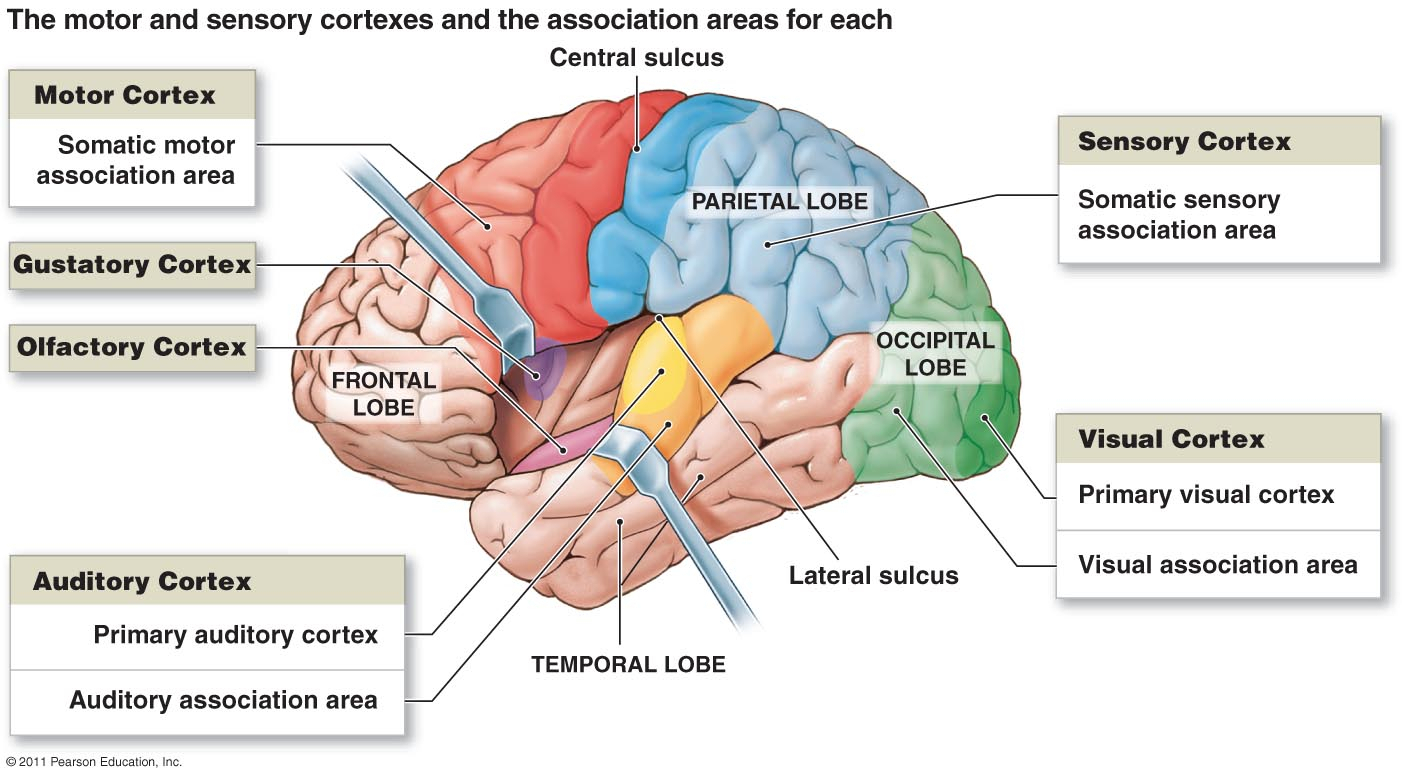
\includegraphics[width=0.65\linewidth]{img/Brain}
	\caption{The human brain.}
	\label{fig:brain}

\end{figure}

The \textit{neuron} model is composed of:
\begin{itemize}
	\item \textit{Soma}, which is the calculation unit
	\item \textit{Axon}, that acts as a transmission line output
	\item \textit{Dendrite} is the input terminal ot the cell that receive messages from other connected cells
	\item \textit{Synapses}: permits a neuron to pass an electrical or chemical signal to another neuron or to the target effector cell.
\end{itemize}

%The Biological neurons are electro-chemical devices, operating at low rates ($\approx mses$).
%Digital circuits operate at very high rates ($\approx nsec$).

\begin{figure}[t]
	\centering
	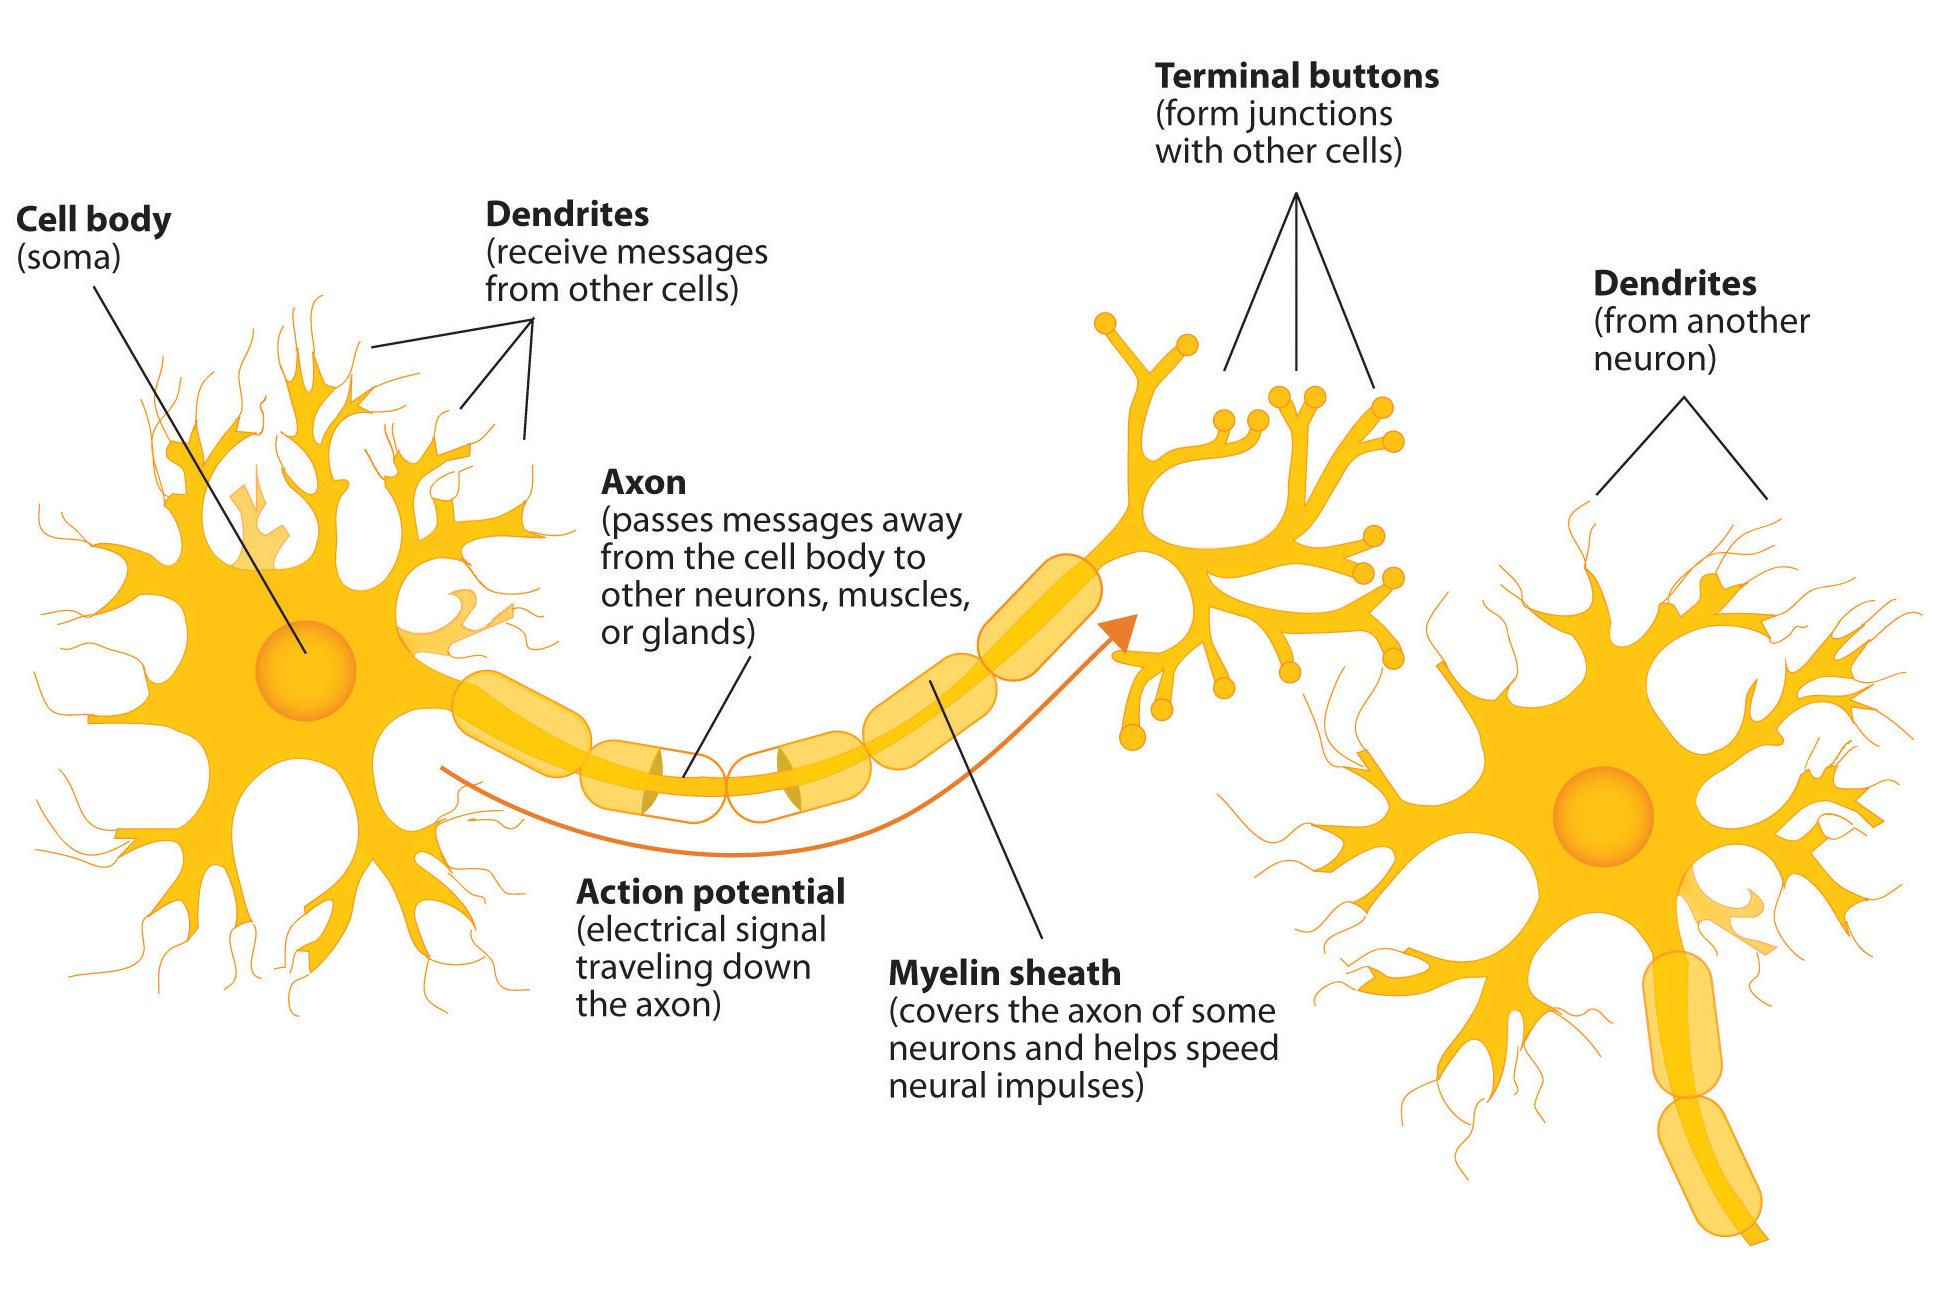
\includegraphics[width=\linewidth]{img/neuron_model}
	\caption{The neuron model.}
	%\label{aa}
\end{figure}

The \textit{neuron} properties can be described in:
\begin{itemize}
	\item \textit{local simplicity}: the neuron receives stimuli (excitation or inhibition) from dendrites and produces an impulse to the axon which is proportional to the weighted sum of the inputs;
	\item \textit{global complexity}: the human brain possess 
	$\mathcal{O}(10^{10})$ 
	neurons, with more than 10K connections each;
	\item \textit{learning}: even though the network topology is relatively fixed, the strength of connections (synaptic weights) can change when the network is exposed to external stimuli;
	\item \textit{distributed control}: no centralized control, each neuron reacts only to its own stimuli;
	\item \textit{tolerance to failures}: performance slowly decrease with the increase of failures.
\end{itemize}

The biological Neural Networks are able to solve very complex tasks in few time instants (like memorization, recognition, association, and so on.)

%\begin{figure}[t]
%	\centering
%	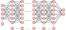
\includegraphics[width=\textwidth]{img/ANN}
%	\caption{The Artificial Neural Network.}
%	%\label{aa}
%\end{figure}

The \textit{Artificial Neural Networks} (ANNs) are defined as \textit{Massively parallel distributed processors made up of simple processing units having a natural propensity for storing experiential knowledge and making it available for use} (Haykin, 2008).

An ANN resembles the brain in two aspects:
\begin{enumerate}
	\item Knowledge is acquired by the network from its environment through a learning process;
	\item Synaptic weights are used to store the acquired knowledge.
\end{enumerate}

An artificial neural network (ANN), is a mathematical/informatical model calculation based on biological neural networks.
This model is constituted by a group of interconnections of information consisting of artificial neurons and processes using a connectionist approach to computation. In most cases, an artificial neural network is an adaptive system that changes its structure, which is based on external or internal information that flows through the network during the learning phase. 
In practical terms neural networks are non-linear structures of statistical data organized as modeling tools.
They can be used to simulate the complex relationships between inputs and outputs that other analytic functions fail to represent.
An artificial neural network receives external signals on a layer of nodes (processing unit) input, each of which is connected with a number of internal nodes, organized in several levels. Each node processes the received signals performing a very simple task  and transmits the result to subsequent nodes. 
\begin{figure}[t]

	\centering
	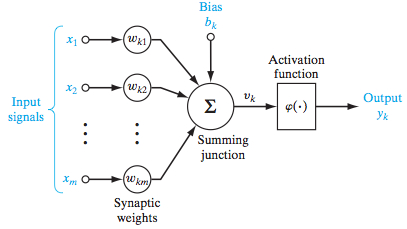
\includegraphics[width=0.8\linewidth]{img/NeuronModel.jpg}
	%\label{aa}
	\caption{The artificial neuron model.}
	\label{fig:artificial_neuron}
\end{figure}

The artificial neuron is an information-processing unit that is fundamental to the operation of a neural network. The model of a neuron is composed of three basic elements, as shown in \figref{fig:artificial_neuron}: 
\begin{itemize}
	\item a \textit{set of synapses}, or connecting links, each of which is characterized by a weight or strength of its own, $w_{km}$; The neural model also includes an externally applied \textit{bias}, denoted by $b_k$.
	\item an \textit{adder} for summing the input signals, weighted by the respective synaptic strengths of the neuron; the operations described here constitute a linear combiner;
	\item an \textit{activation function} for limiting the amplitude of the output of a neuron. Typically, the normalized amplitude range of the output of a neuron is written as the closed unit interval [0,1], or, alternatively, [-1,1].
\end{itemize}
The neural model also includes an externally applied \textit{bias}, denoted by $b_k$.



Therefore, the mathematical description of neuron activity can be defined as:
\begin{eqnarray}
{ u }_{ k }=\sum _{ j=1 }^{ m }{ { w }_{ kj } } { x }_{ j }\\ 
{ y }_{ k }=\varphi \left( { u }_{ k }+b_{ k } \right)
\end{eqnarray}
where:
\begin{itemize}
	\item ${ x }_{ 1 },{ x }_{ 2 },\cdots ,{ x }_{ m }$ are the input signals;
	\item ${ w }_{ k1 },{ w }_{ k2 },\cdots ,{ w }_{ km }$ are the respective synaptic weights of neuron $k$;
	\item $u_k$ is the linear combiner output due to the input signals;
	\item $b_k$ is the bias;
	\item $\varphi(\cdot)$ is the activation function;
	\item $y_k$ is the output signal of the neuron.
\end{itemize}

The types of \textit{activation non-linear functions} $\varphi(x)$ are:
\begin{itemize}
	
	\item the \textit{threshold function}: in engineering, this form of a threshold function is commonly referred to as a Heaviside function;
	\begin{eqnarray}
	\varphi \left( v \right) =1\quad if\quad v\ge 0 \\ 
	\varphi \left( v \right) =0\quad if\quad v<0
	\end{eqnarray}
	\begin{figure}
		\centering
		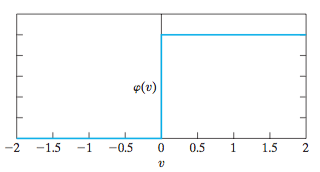
\includegraphics[width=0.4\textwidth]{img/Heaviside}
		\caption{The threshold non-linear function.}
		%\label{aa}
	\end{figure}
	
	\item the \textit{sigmoid function}: it is defined as a strictly increasing function that exhibits a graceful balance between linear and nonlinear behavior; an example of the sigmoid function is the \textit{logistic function} defined by:
	\begin{equation}
	\varphi \left( v \right) =\frac { 1 }{ 1+exp\left( -av \right)  } 
	\end{equation}
	\begin{figure}
		\centering
		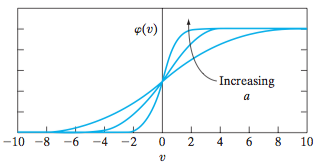
\includegraphics[width=0.4\textwidth]{img/sigmoid}
		\caption{The sigmoid non-linear function.}
		%\label{aa}
	\end{figure}
	
	\item the \textit{ hyperbolic tangent } ($tanh$): it is simply a scaled and shifted version of the sigmoid function:
	\begin{equation}
	\varphi(x) = \frac{1-e^{-2x}}{1+e^{-2x}}
	\end{equation}
	\begin{figure}[t]
		\centering
		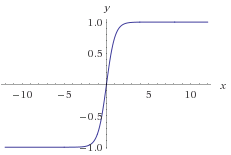
\includegraphics[width=0.4\textwidth]{img/tanh}
		\caption{The $tanh$ non-linear function.}
		%				\label{aa}
	\end{figure}
	
	\item the \textit{ Rectifier Linear Unit} ($ReLU$):
	\begin{equation}
	\varphi(x) = \text{max}(0,x)
	\end{equation}
	\begin{figure}[t]
		\centering
		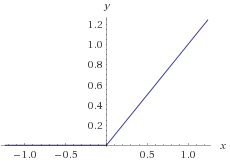
\includegraphics[width=0.4\textwidth]{img/relu}
		\caption{The $ReLU$ non-linear function.}
		%				\label{ee}
	\end{figure}
	
	\item the $softmax$: it is used on the last layer of a classifier setup: the outputs of the softmax layer represent the probabilities that a sample belongs to the different classes. Indeed, the sum of all the output is equal to $1$.
	%In this case the targets are \textit{one-hot} vectors and the cost-function is the \textit{categorical cross-entropy}.
	\begin{equation}
	\varphi(x_k) = \frac{e^{x_k}}{\sum_{j=1}^{N}e^{x_j}} \text{ for }  k=1,\dots,K
	\end{equation}
	\begin{figure}[t]
		\centering
		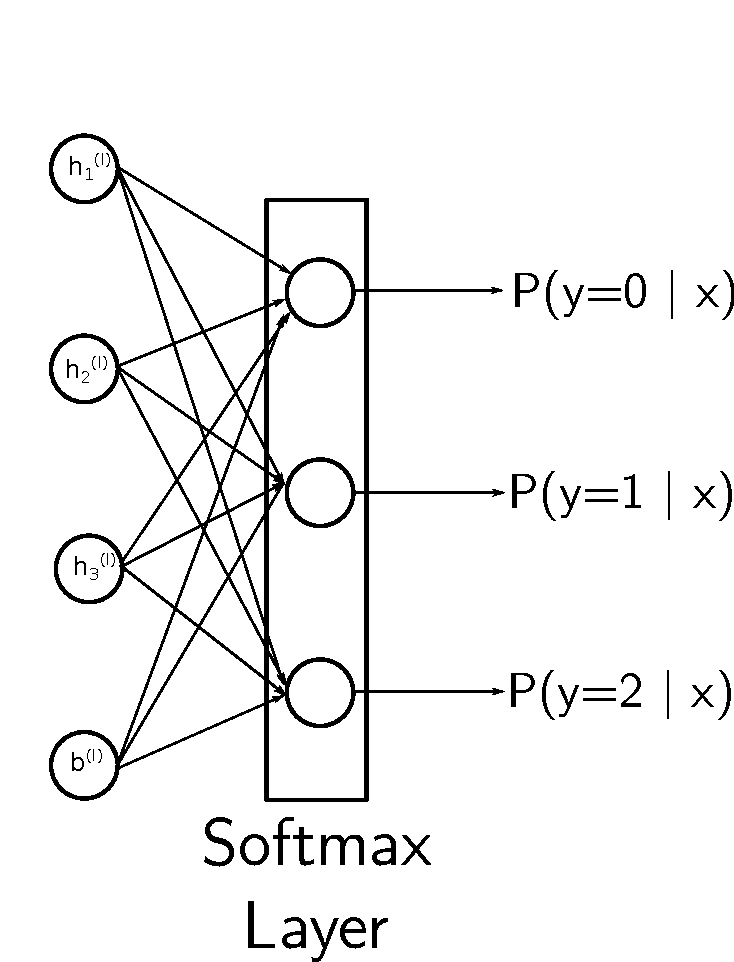
\includegraphics[width=0.4\textwidth]{img/softmax}
		\caption{The $\textit{softmax}$ layer in a neural network classifier.}
		%					\label{aa}
	\end{figure}	
	
	%			\item $\mathbf{maxout}$ - the output is the maximum value among $K$ linear models applied to a given input (or an hidden activation): $\varphi(x_k) = \max(x_k)$ with $k=1,\dots,K$.\\
	%			It is supposed to be combined with dropout.
	
	%		It is an approximate model averaging technique. A single maxout unit performs a piecewise linear approximation to an arbitrary convex function. Maxout networks learn not just the relationship between hidden units, but also the activation function of each hidden unit.	
	
	
	
	%				\begin{figure}
	%				\centering
	%					\includegraphics[width=0.75\textwidth]{img/maxout}
	%					\caption{Example of an MLP with $\mathbf{maxout}$ units. Picture courtesy of GoodFellow et al. 2013}
	%%					\label{rr}
	%				\end{figure}
	
\end{itemize}

% ****************************************************+
%NEURAL NETWORKS VIEWED AS DIRECTED GRAPHS
%
%A neural network is a \textbf{directed graph} consisting of nodes with interconnecting synaptic and activation links and is characterized by four properties:
%
%\begin{enumerate}
%\item Each neuron is represented by a set of linear synaptic links, an externally applied bias, and a possibly nonlinear activation link. The bias is represented by a synaptic link connected to an input fixed at $+1$.
%\item The synaptic links of a neuron weight their respective input signals.
%\item The weighted sum of the input signals defines the induced local field of the neuron in question
%\item The activation link squashes the induced local field of the neuron to produce an output
%\end{enumerate}
%
%\begin{figure}
%\centering
%\includegraphics[width=0.55\textwidth]{img/NeuronGraph.jpg}
%\caption{The Neuron graph model.}
%%\label{key}
%\end{figure}
%
%When the focus of attention is restricted to signal flow from neuron to neuron, we may use a reduced form of this graph by omitting the details of signal flow inside the individual neurons. Such a directed graph is said to be \textit{partially complete}. It is characterized as follows:
%
%\begin{enumerate}
%\item Source nodes supply input signals to the graph.
%\item Each neuron is represented by a single node called a computation node.
%\item The communication links interconnecting the source and computation nodes of the graph carry no weight; they merely provide directions of signal flow in the graph.
%\end{enumerate}
%
%%\begin{figure}
%%\centering
%%\includegraphics[width=0.55\textwidth]{img/NeuronPGraph.jpg}
%%%\label{aa}
%%\caption{ee}
%%\end{figure}
%
%
%Graphical representations of a neural network
%
%\begin{itemize}
%\item \textbf{Block Diagram} $\rightarrow$ functional description of the network
%\item \textbf{Architectural Graph} $\rightarrow$ description of the network layout
%\item \textbf{Signal-Flow Graph} $\rightarrow$ complete description of the signal flow in the network
%\end{itemize}

% *********************************************************+

In past years, many models of neurons and neural architectures have been proposed in the literature, each with its peculiarities. A brief description of the leading models used in the works described in the following chapters will now be given:
\begin{enumerate}
	
	%\item \textit{Single-Layer Feedforward Networks} (SLFN):
	%
	%\begin{itemize}
	%\item We have an input layer of source nodes that projects directly onto an output layer of neurons (computation nodes), but not vice-versa 
	%\item Such a network is called a single-layer network, with the designation \emph{single-layer} referring to the output layer of computation nodes (neurons). 
	%\item We do not count the input layer of source nodes because no computation is performed there.
	%\end{itemize}
	%
	%\begin{figure}
	%\centering
	%\includegraphics[width=0.35\textwidth]{img/SLFN}
	%%\label{aa}
	%\caption{The Single-Layer Feedforward Network.}
	%\end{figure}
	
	
	\item \textit{Multilayer Feedforward Networks} - (FFNN):
	
	it is characterized by the presence of one or more hidden layers, whose computation nodes are correspondingly called \textit{hidden neurons} (or hidden units);
	the term \textit{hidden} refers to the fact that this part of the neural network is not seen directly from either the input or output of the network. 
	The function of hidden neurons is to intervene between the external input and the network output in some useful manner. By adding one or more hidden layers, the network is enabled to extract higher-order statistics from its input. 
	%\item Example: \textbf{10-4-2 network} $->$ it has 10 source nodes, 4 hidden neurons, and 2 output neurons.
	
	
	\begin{figure}
		\centering
		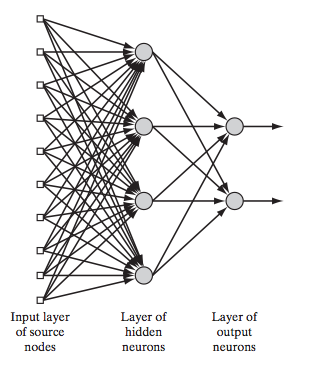
\includegraphics[width=0.4\textwidth]{img/MLP}
		%\label{aa}
		\caption{The Multilayer Feedforward Network.}
	\end{figure}
	
	
	%\textbf{ndRob} to complete, 1 pages with figure
	%\begin{itemize}
	%\item struttura a layer
	%\item notazione matriciale con indici layer
	%\end{itemize}
	
	The MLP is a well known kind of artificial neural network introduced in 1986 \cite{Rumelhart86-LRB}. 
	Each node applies an activation function over the weighted sum of its inputs. 
	The units are arranged in layers, with feed forward connections from one layer to the next. 
	The stochastic gradient descent with error back-propagation algorithm is used for the supervised learning of the network. 
	In the forward pass, input examples are fed to the input layer, and the resulting output is propagated via the hidden layers towards the output layer. At the backward pass, the error signal originating at the output neurons is sent back through the layers and the network parameters (i.e., weights and biases) are tuned.
	
	A single neuron can be formally described as:
	\begin{equation}
	%g(\mathbf{u}[n])=\varphi \left(\left(\begin{matrix} \sum _{ j=1 }^{ D }{w_j u_j[n] }  \end{matrix} \right) + b\right),
	g(\mathbf{u}[n])=\varphi \left(\sum _{ j=1 }^{ D }{w_j u_j[n] } + b\right),
	\end{equation}
	where $\mathbf{u}[n] \in \mathbb{R}^{D\times 1}$, the bias $b$ is an externally applied term and $\varphi(\cdot)$ is the non-linear activation function.
	Thus, the mathematical description of a one-hidden-layer MLP is a function $\mathbf{f}:\mathbb{R}^D \rightarrow \mathbb{R}^{D'}$, where $D'$ is the size of the output vector, so:
	\begin{equation}
	\mathbf{f}(\mathbf{u}[n]) = 	\varphi \left( \mathbf{b}_2 + \mathbf{W}_2 \left( \varphi \left( \mathbf{b}_1 + \mathbf{W}_2 \cdot \mathbf{u}[n]\right) \right) \right),
	\end{equation}
	where $\mathbf{W}_i$ and $\mathbf{b}_{i}$ are the respective synaptic weights matrix and the bias vector of the $i$-th layer.
	The behaviour of this architecture  is  parametrized  by  the connection weights, which are adapted during the supervised network training.
	
	
	
	\item \textit{Convolutional Neural Networks}(CNN)
	
	\begin{figure}
		\centering
		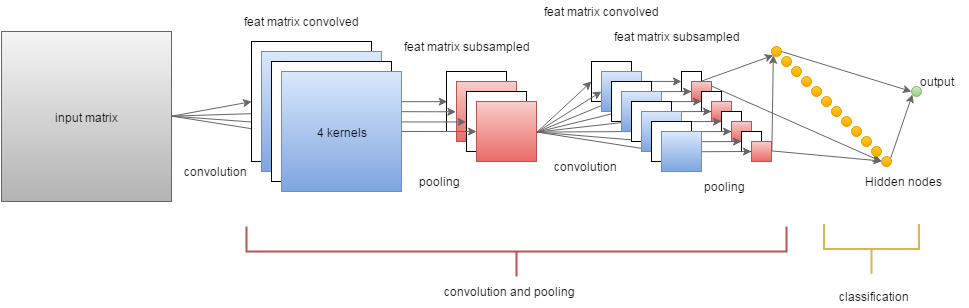
\includegraphics[width=0.9\columnwidth]{img/CNN}
		%	 \label{ee}
		\caption{The Convolutional Neural Network.}
	\end{figure}
	
	%\textbf{ndRob} to complete,  1 pages with figure
	
	Convolutional neural networks are feedforward neural networks similar to multilayer perceptron, with some special layers.
	
	%Matrix convolution: it is performed between a bigger matrix, which is the input, and a smaller matrix, the convolutional kernel.
	
%	\begin{figure}[t]
%		\centering
%		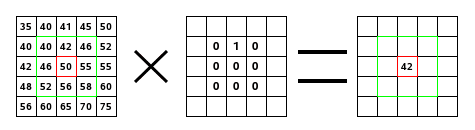
\includegraphics[width=0.7\columnwidth]{img/convolution-calculate}
%		%		\label{ee}
%		\caption{The convolution operation.}
%	\end{figure}
	
	
	
	%	\item Convolution kernels, by training, adapt on recurrent input patterns, becoming themselves similar to those patterns. As a result an activation of the kernel is given when a specific pattern occurs. 
	Convolution kernels process the input data matrix by dividing it in \textit{local receptive fields}, a region of the same size of the kernel, and sliding the local receptive field across the entire input.
	Each hidden neuron is thus connected to a local receptive field, and all the neurons form a matrix called \textit{feature map}.
	%We can have multiple feature maps.
	The weights in each \textit{feature map} are \textit{shared}: all hidden neurons are aimed to detect exactly the same pattern just at different locations in the input image. 
	
	The main advantages of this network is the robust pattern recognition system characterized by a strong immunity to pattern shifts.
	
	Pooling layer just reduces the dimension of the matrix by a rule: a submatrix of the input is selected, and the output is the maximum value of this submatrix.
	
%	\begin{figure}
%		\centering
%		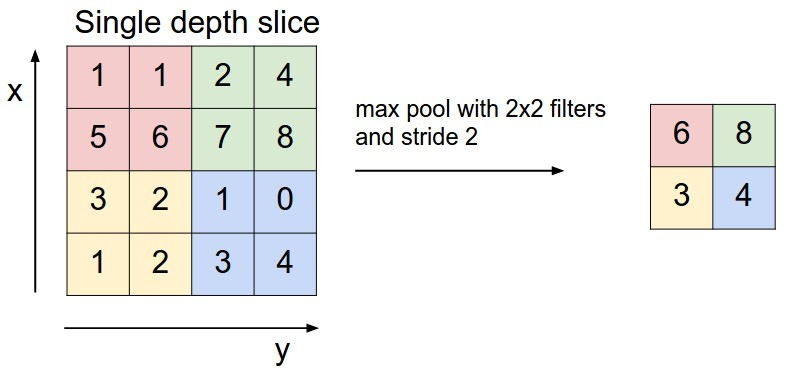
\includegraphics[width=0.6\columnwidth]{img/maxpool.jpeg}
%		%		\label{rr}
%		\caption{The max-pooling layer.}
%	\end{figure}
	
	The pooling process introduces tolerance against shifts of the input patterns. Together with convolution layer it allows the CNN to detect if a particular event occurs, regardless its deformation or its position.
	
	CNN is a feed-forward neural network \cite{lecun1998gradient} usually composed of three types of layers: convolutional layers, pooling layers and layers of neurons.
	The convolutional layer performs the mathematical operation of convolution between a multi-dimensional input and a fixed-size kernel. Successively, a non-linearity is applied element-wise. 
	%In the convolution process the kernel moves all along the input matrix and, for each position, every element of the kernel is multiplied with the corresponding one on the input matrix. All the values are finally summed.
	The kernels are generally small compared to the input, allowing CNNs to process large inputs with few trainable parameters.
	%From the input matrix, for each convolutional kernel, a new matrix is obtained, also called \textit{feature map}.
	Successively, a pooling layer is usually applied, in order to reduce the feature map dimensions. One of the most used is the \textit{max-pooling} whose aim is to introduce robustness against translations of the input patterns.
	%Different strategies are available for pooling, but we only consider max-pooling, which selects the maximum value in a sub-matrix of the input and discards the other values. Pooling introduces toughness against shifts of the input patterns. 
	Finally, at the top of the network, a layer of neurons is applied. This layer does not differ from MLP, being composed by a set of activation and being fully connected with the previous layer. For clarity, the units contained in this layer will be referred as \textit{Hidden Nodes} (HN).
	
	Denoting with $\mathbf{W}_{m} \in \mathbb{R}^{K_{1m}\times K_{2m}}$ the $m$-th kernel and with $\mathbf{b}_{m}  \in \mathbb{R}^{D_1\times D_2}$ the bias vector of a generic convolutional layer, the $m$-th feature map  $\mathbf{h}_{m} \in \mathbb{R}^{D_1\times D_2}$ is given by:
	\begin{equation}\label{eq:backg:dnn:conv_op}
	%h_{m,i}=\varphi	\left(W_{m,i} \ast \mathbf{u}_j[n] + b_{m,i} \right),
	\mathbf{h}_{m}=\varphi	\left(\sum_{d=1}^{D_3} \mathbf{W}_{m} \ast \mathbf{u}_d + \mathbf{b}_{m} \right),
	\end{equation}
	where $\ast$ represent the convolution operation, and $\mathbf{u}_{d} \in \mathbb{R}^{D_1\times D_2} $ is a matrix of the three-dimensional input tensor $\mathbf{u} \in \mathbb{R}^{D_1\times D_2 \times D_3}$. The dimension of the $m$-th feature map $\mathbf{h}_{m}$ depends on the zero padding of the input tensor: here, padding is performed in order to preserve the dimension of the input, i.e., $\mathbf{h}_{m} \in \mathbb{R}^{D_1\times D_2}$. Please note that for the sake of simplicity, the time frame index $n$ has been omitted.  %The different feature maps obtained from each kernel of a convolutional layer are then summed to compose the input data for the following layer.
	Commonly, \eqref{eq:backg:dnn:conv_op} is followed by a pooling layer in order to be more robust against patterns shifts in the processed data, e.g. a max-pooling operator that calculates the maximum over a $P_1 \times P_2 $ matrix is employed.
	
\end{enumerate}


A \textit{Deep Learning} definition: \textit{A  class  of  machine learning  techniques  that
	exploit  many  layers  of  non-linear  information  processing  for supervised  or  unsupervised  feature  extraction  and  transformation, and for pattern analysis and classification.}
%...we need complex networks to deal with the \textit{feature representation learning} paradigm.
Artificial Neural Networks are often referred as deep when they have more than 1 or 2 hidden layers.
%		\item Important Issues
%		\begin{itemize}
%			\item Rule of Thumb: \textit{for a given performance rate on the testing data, the amount of training data and the number of free parameters are directly proportional}.
%			\item Do we have enough data for training and to achieve a satisfying generalization performance?
%			\item How to select the ``right'' model? 
%		\end{itemize}


\subsection{Stochastic gradient descent (SGD)}

Most deep learning training algorithms involve optimization of some sort.
The most widely used is the gradient based optimization, which belongs to the first order type.

\textit{Optimization} is the task of either minimizing some function $f(x)$ by altering $x$:
$f(x)$ is called \textit{objective function}, but in the case when it has to be minimized, it is also call the \textit{cost function}, \textit{loss function}, or \textit{error function}.
The aim of the optimization is reached doing small change $\epsilon$ in the input $x$, to obtain the corresponding change in the output $f(x)$:
\begin{equation}
f(x+\epsilon) \approx f(x)+\epsilon\,f'(x).
\end{equation}
This formulation is based on the calculation of the derivative $f'(x)$.
The \textit{gradient descent} is the technique based on the reduction of $f(x)$ by moving $x$ in small steps with the opposite sign of the derivative.
The aim is to find the minimum of the cost function: when $f'(x)=0$, the derivative provides no information about which direction to move, therefore this point is defined as stationary points.
A local minimum is a point where $f(x)$ is lower than at all neighbouring and it is no longer possible to decrease $f(x)$ by making infinitesimal steps.
The absolute lowest value of $f(x)$ is a \textit{global minimum}.

For the concept of minimization to make sense, there must still be only one (scalar) output.
For functions that have multiple inputs $f: \R^n \rightarrow \R$, the concept of \textit{partial derivatives} is introduced.
The gradient $\nabla_{\mathbf{x}}f(\mathbf{x})$ is the vector containing all the partial derivatives.

The method of \textit{steepest descent} or \textit{gradient descent} states that decrease $f$ by moving in the direction of the negative gradient.
\begin{equation}
\textbf{x'} = \textbf{x} - \epsilon\,\nabla_{\mathbf{x}}f(\mathbf{x}),
\end{equation}
where $\epsilon$ is the \textit{learning rate}, a positive scalar determining the size of the step.

Large training sets are necessary for good generalization, but large training sets are also more computationally expensive.
The cost function decomposes as a sum over training example of per-example loss function:
i.e., the negative conditional log-likelihood of the training data is defined as:
\begin{equation}
J(\mathbf{\theta}) = \mathbb{E}(L(\textbf{x}, y, \mathbf{\theta})) = \frac{1}{m} \sum\limits_{i=1}^{m} L(\textbf{x}^{(i)}, y^{(i)}, \mathbf{\theta}),
\end{equation}
where $L$ is the per-example loss $L(\textbf{x}, y, \mathbf{\theta}) = - \log p(y|\textbf{x};\mathbf{\theta})$.
The gradient descent requires computing:
\begin{equation}
\nabla_{\theta} J(\mathbf{\theta}) = \frac{1}{m} \sum\limits_{i=1}^{m} \nabla_{\theta} L(\textbf{x}^{(i)}, y^{(i)}, \mathbf{\theta}).
\end{equation}
The computational cost of this operation is proportional to the number of example $m$, therefore as the training set size grows the time to take a single gradient step becomes prohibitively long.

\textit{Stochastic gradient descent} (SGD) is an extension of the gradient descent algorithm: the insight is that the gradient is an expectation estimated using a small set of samples.
On each step of the algorithm, a sample of example $\mathbb{B} = \{ \textbf{x}^{(1)}, \ldots, \textbf{x}^{(m')}\}$, called \textit{minibatch}, is drawn uniformly from the training set.
The minibatch size $m'$ is typically chosen to be a relatively small number of examples.
The estimate of the gradient is:
$\textbf{g} = \frac{1}{m'} \nabla_{\theta} \sum\limits_{i=1}^{m'} L(\textbf{x}^{(i)}, y^{(i)}, \mathbf{\theta})$
using examples from the minibatch $\mathbb{B}$.
The SGD algorithm then follows the estimated gradient downhill:
\begin{equation}
\theta \leftarrow \theta - \epsilon\,\textbf{g}
\end{equation}
where $\epsilon$ is the learning rate.

%\textbf{ndRob} to be inserted: tipo di loss function MSE, come si calcola su uscita 

%\textbf{ndRob} to complete, learning for FF e CNN (in slides)




\subsection{Autoencoder}
\label{sec:autoencoder_theory}
%\textbf{ndRob} to complete, 1-2 pages with figures
%
%\begin{itemize}
%\item definition
%\item notazione matriciale
%\item denoising Auto Encoder (dAE)
%\end{itemize}



An Autoencoder is a kind of neural network typically consisting of only one hidden layer, trained to set the target values to be equal to the inputs.
\begin{equation} %\label{eq:layer2}
\tilde{x} = f(W_{2}h(x) +b_{2})
\end{equation}

%\begin{figure}
%\centering
%\includegraphics[width=0.65\textwidth]{img/basic_AE}
%%\label{ee}
%\caption{rr}
%\end{figure}


Given an input set of examples $\mathcal{X}$, autoencoder training consists
in finding parameters $\theta=\{W_{1},W_{2},b_{1},b_{2}\}$ that
minimize the Reconstruction Error:
\begin{equation}\label{eq:obAE}
\mathcal{J}(\theta)=\sum_{x\in{\mathcal{X}}}\left\| x - \tilde{x}\right\|^{2}
\end{equation}

Defining $M$ the number of hidden units, and $N$ the number of input units, output units, features size:

\begin{figure}
	\centering
	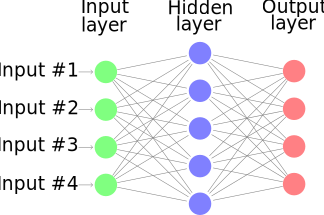
\includegraphics[width=\columnwidth]{img/autoencoder}
	\caption{The different types of Autoencoders.}
	\label{fig:backg:dnn:AE}
\end{figure}

\begin{itemize}
	\item (a):  $M=N \rightarrow$ Basic Autoencoder (AE);
	\item (b):  $M<N \rightarrow$ Compression Autoencoder (CAE);
	\item (c):  $M>N$ and Gaussian Noise $\rightarrow$ Denoising Autoencoder (DAE);
\end{itemize}


%This section introduces the concepts of autoencoders and describes the basic autoencoder, compression autoencoder, de-noising autoencoder, and non-linear predictive autoencoder.

An AE -- a kind of neural network typically consisting of only one hidden layer --, sets the target values to be equal to the input. It is used to find common data representation from the input \cite{Goodfellow2009-MII,Bengio2007-GLT}. Formally, in response to an input example $x\in \mathbf{R}^{n}$, the hidden representation
$h(x) \in \mathbf{R}^{m}$ is 
\begin{equation} %\label{eq:layer1}
h(x) = f(W_{1}x +b_{1}), 
\end{equation}
where $f(z)$ is a non-linear activation function, typically a logistic
sigmoid function $f(z) = 1/(1+\exp(-z)) $ applied component-wisely,
$W_{1} \in \mathbf{R}^{m \times n}$ is a weight matrix, and $b_{1} \in
\mathbf{R}^{m}$ is a bias vector.

The network output maps the hidden representation $h$ back to a
reconstruction $\tilde{x} \in \mathbf{R}^{n}$:
\begin{equation} %\label{eq:layer2}
\tilde{x} = f(W_{2}h(x) +b_{2}), 
\end{equation}
where $W_{2} \in \mathbf{R}^{n \times m}$ is a weight matrix, and $b_{2} \in
\mathbf{R}^{n}$ is a bias vector.

Given an input set of examples $\mathcal{X}$, AE training consists
in finding parameters $\theta=\{W_{1},W_{2},b_{1},b_{2}\}$ that
minimise the reconstruction error, which corresponds to minimising
the following objective function:
\begin{equation} %\label{eq:obAE}
\mathcal{J}(\theta)=\sum_{x\in{\mathcal{X}}}\left\| x -
\tilde{x}\right\|^{2}.
\end{equation}
The minimisation is usually realised by stochastic gradient descent as
in the training of neural networks. The structure of the AE is given in \figref{fig:backg:dnn:AE}a.   


%\subsection{Siamese Neural Network}




\graphicspath{{3_datasets/}}
\chapter{Dataset}
\label{ch:dataset}
%poichè non erano presnti dataset adui suabili, ce ne siamo fatti uno noi. Poi per ogni metodo verranno esplicitati i dati usati.

The importance of using public data sets for algorithm evaluation is very important. Only in this way can a direct comparison be made between the different approaches to determine which of these is actually the best. There are publicly available datasets for the fall detection task, the majority of them are all related to wearable or vision sensors and often include both types \cite{spinsantefalldata, kwolek2014human, charfi2013optimized, s140610691, s17071513}.  Since in this work, we face the problem of human fall detection from an audio perspective, a preliminary search for datasets containing audio signals has been performed. Only one dataset containing audio recording has been found \cite{cirdodataset}. However, the audio files available in the dataset are suitable for speech recognition related works rather than sound event detection. In fact, only the utterance of short sentences or interjections of the actors involved during the human falls recordings have been annotated.   Although the principal limitation in that the human falls were made by volunteers by using various protections, which do not allow the correct acquisition of the acoustic pattern produced by the sound event.  As in this work, several data-driven approaches for pattern recognition produced by the sound generated by the human fall are presented, the dataset \cite{cirdodataset} result useless. Given the lack of available audio datasets, we have created a suitable one in order to assess the proposed approaches. This choice was also forced by the fact that in these works an innovative acoustic sensor explicitly developed for the fall detection and described in \secref{sec:sensor} has been used.
In this chapter, the instrumentation, the procedure for recording the audio corpus and its composition are described.

\section{The floor acoustic sensor}
\label{sec:sensor}

\begin{figure}[t]
	\centering
	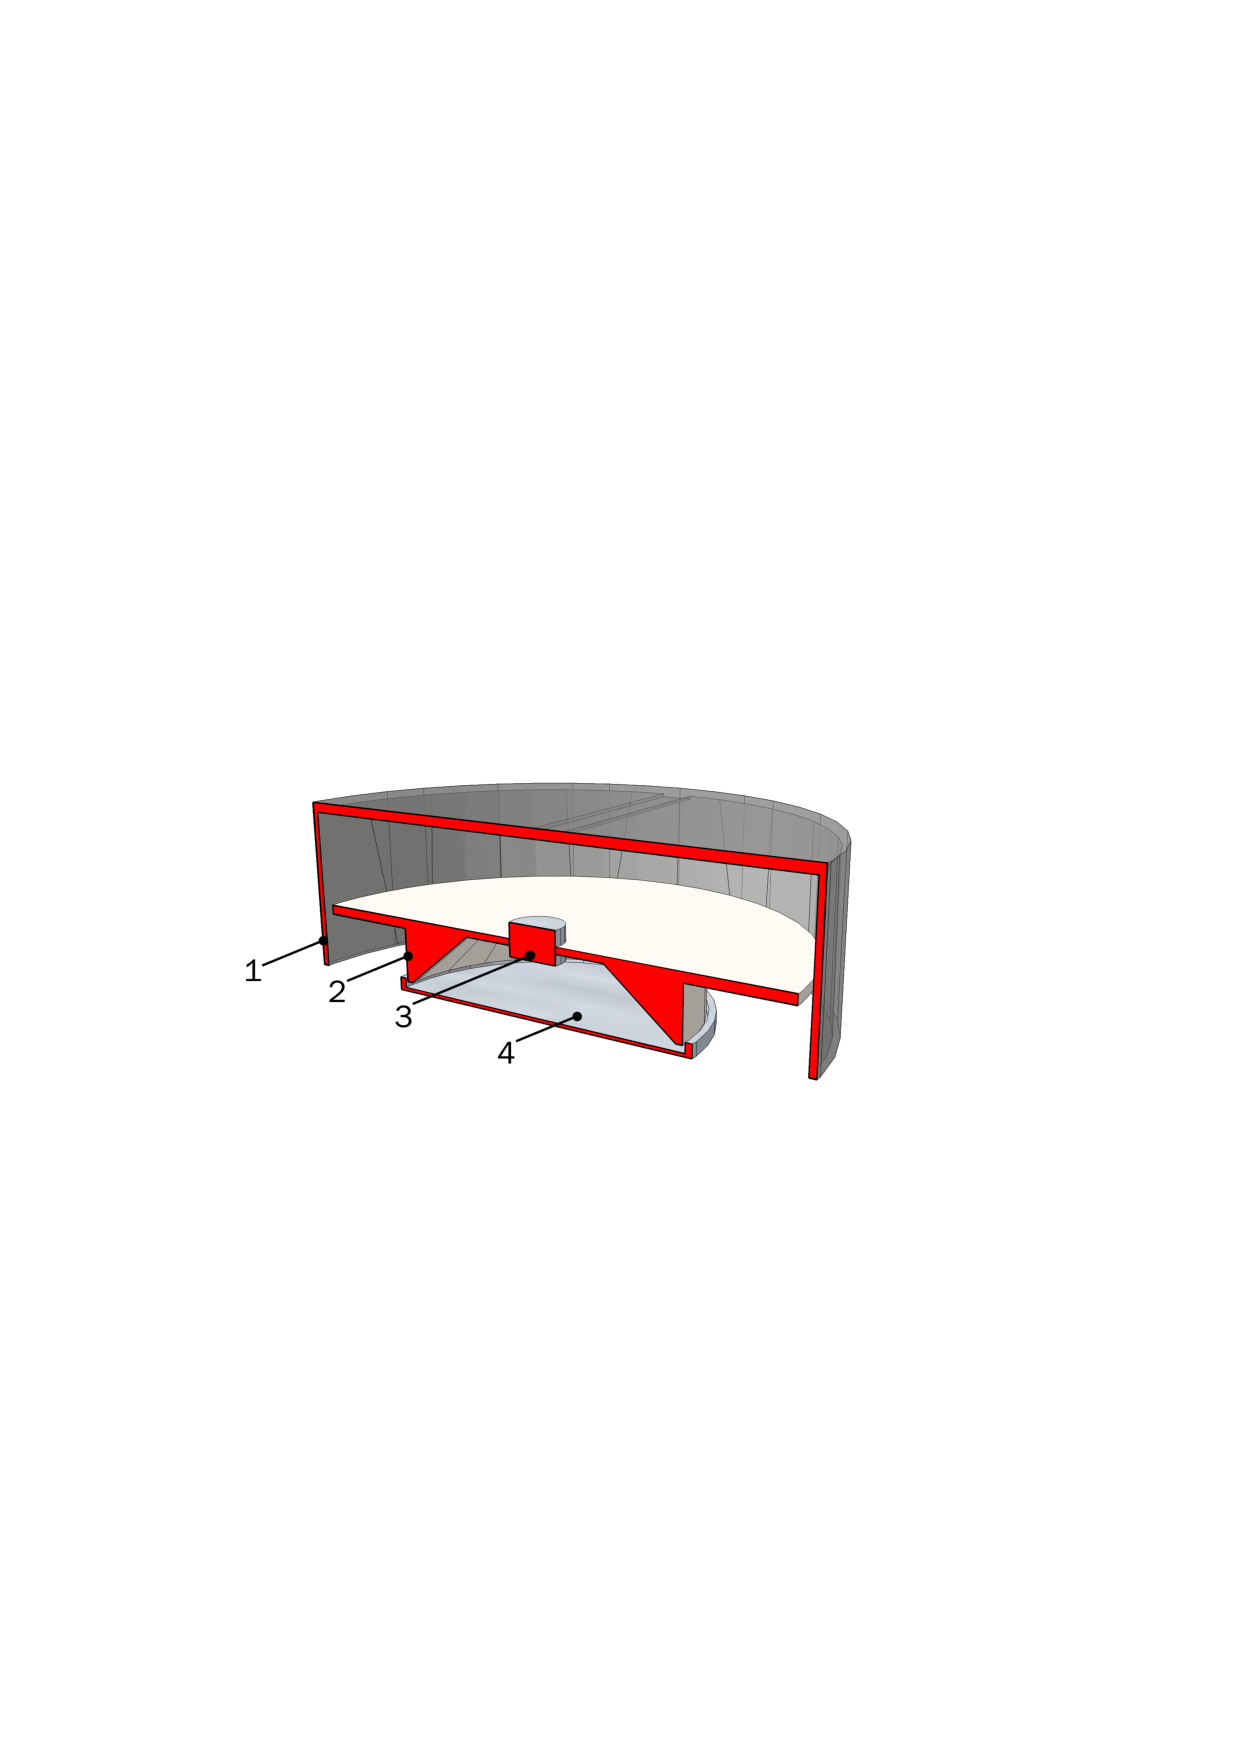
\includegraphics[width=0.8\textwidth]{img/AcousticSensor.pdf}
	\caption{The floor acoustic sensor: conceptual scheme. \mbox{1 - The} outer container. \mbox{2 - The} inner container. \mbox{3 - The} microphone slot. \mbox{4 - The} membrane touching the floor.}
	\label{fig:case}
\end{figure}
The floor acoustic sensor (FAS) is composed of a resonant enclosure and a microphone located inside it (\figref{fig:case}) \cite{Olivetti15}. At the bottom of  the enclosure, a membrane  is in direct contact with the floor and guarantees the acoustic coupling with the surface. The inner container accommodates the microphone and is where the acoustic resonance phenomenon takes place. It can be covered by a layer of acoustic isolation material and it is enclosed by the outer container that further reduces the intensity of the acoustic waves that propagate through air. The enclosure has been manufactured in Polylactic Acid with a 3D printer, its diameter is 16.5\,cm and its height 5.5\,cm.

%The acoustic sensor used in the sound database acquisition (as described in \secref{Experiments}) is depicted in \figref{fig:meringa}. The dimensions of the acoustic sensor are the following: 16.5\,cm of diameter and 5.5\,cm of height. The material used for the sensor case, developed through the 3D printing technology, is Polylactic Acid. %No acoustic isolation material has been inserted into the space between the inner and outer container.

Regarding the microphone, an AKG C 400 BL\footnote{http://www.akg.com/pro/p/c400-bl} has been inserted in the enclosure. The outer case of the microphone has been removed to extract the capsule that has then been inserted in the sensor enclosure. The AKG C 400 BL is characterized by an hypercardiod directivity pattern, thus it has been oriented so that the maximum gain is towards floor.

\begin{figure}[t]
	\centering
	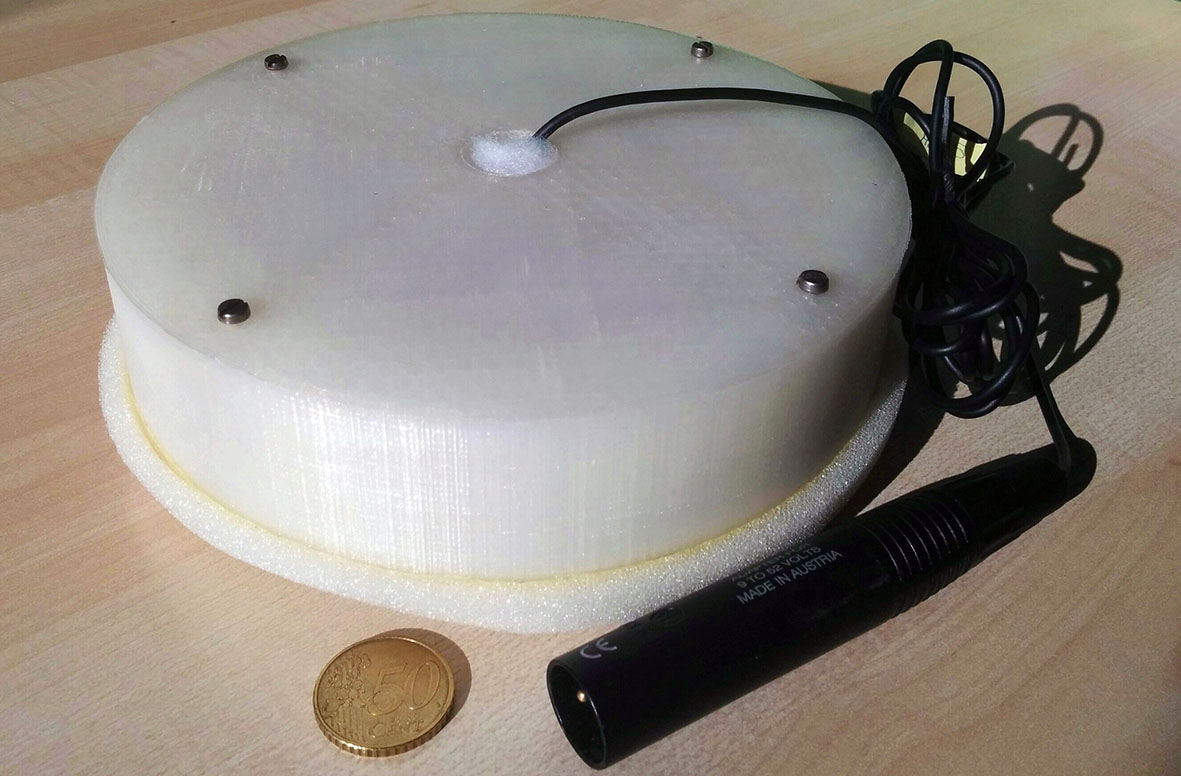
\includegraphics[width=0.8\columnwidth]{img/FAS_front_little.jpg}
	\caption{A picture of the floor acoustic sensor used during the recordings.} 
	\label{fig:meringa}
\end{figure}

\section{The fall events dataset: A3Fall}
\label{sec:dataset}
The performance of the floor acoustic sensor has been evaluated on a corpus of audio events corresponding to falls of several objects recorded in different conditions\footnote{The dataset is available at the following URL: \url{http://www.a3lab.dii.univpm.it/research/fasdataset}}. The dataset has been specifically created by the authors and it will be presented in this section.

\subsection{The recording setup}
Fall events have been recorded in 3 different rooms with the following characteristics:
\begin{itemize}
	\item The first, is a rectangular room, hereafter named R0, measuring about 7\,m\,$\times$\,2\,m (\figref{fig:room}). The room is particularly suitable for the propagation of acoustic waves through the floor since it is obtained from a cantilever beam. In addition, the considerable distance of the supporting pillars facilitates the transmission of a fall vibrations through the floor.
	\item the second location for the recording was the university auditorium room (R1) in which the flooring is composed of fitted carpet (\figref{fig:room1}). This makes it particularly suitable for evaluating system performance on surfaces with acoustical behavior that can mitigate the impact sound transmitted through the floor and in the air; all the recordings were performed near the auditorium stage in an area of 8$\times$3\,m.
	\item a recording studio (R2) was selected as the third location for its particular characteristics (\figref{fig:room2}). Here, it was possible to make the acquisitions by placing the sensors in the live room while the audio events were performed in the control room. In particular, the sensors were positioned immediately behind the soundproof wall with the window overlooking the live room. The size of the live room is 5$\times$7\,m, while the size of the control room is 3$\times$8\,m.
\end{itemize}

  The recording equipment comprises the floor sensor, a linear array of three aerial microphones (the same AKG 400 BL included in the floor sensor) and a Presonus AudioBox 44VSL sound card connected to a laptop. The microphones of the array are separated by 4\,cm and positioned on a table 80\,cm high. Signals were sampled at 44.1\,kHz with a resolution of 32\,bits. Levels were calibrated to assure the maximum dynamic range at the smallest distance.
  
\begin{figure}[htb]
	\centering
	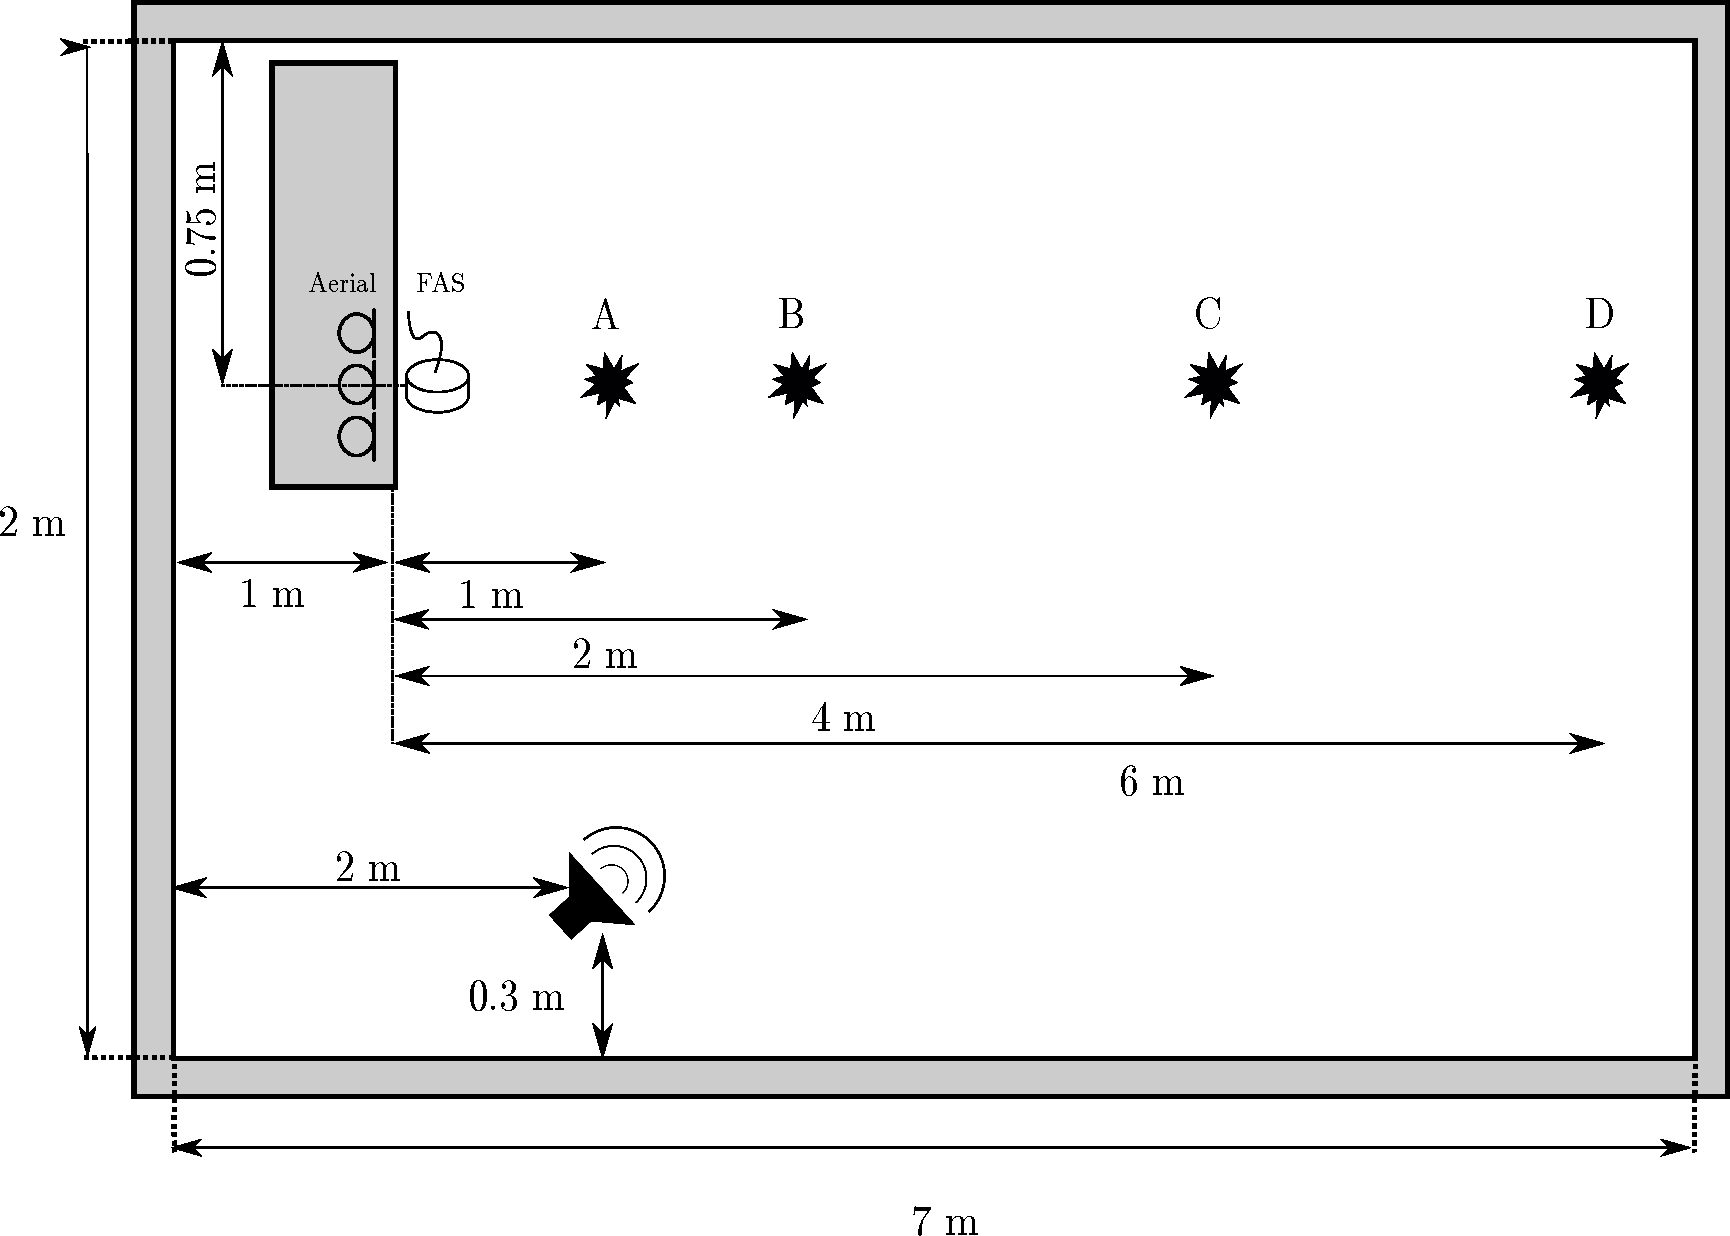
\includegraphics[width=\columnwidth]{img/room_experiments.pdf}
	\caption{The scheme the R0 room: the letters A, B, C and D indicate the positions of fall events.}
	\label{fig:room}
\end{figure}
\begin{figure}[htb]
	\centering
	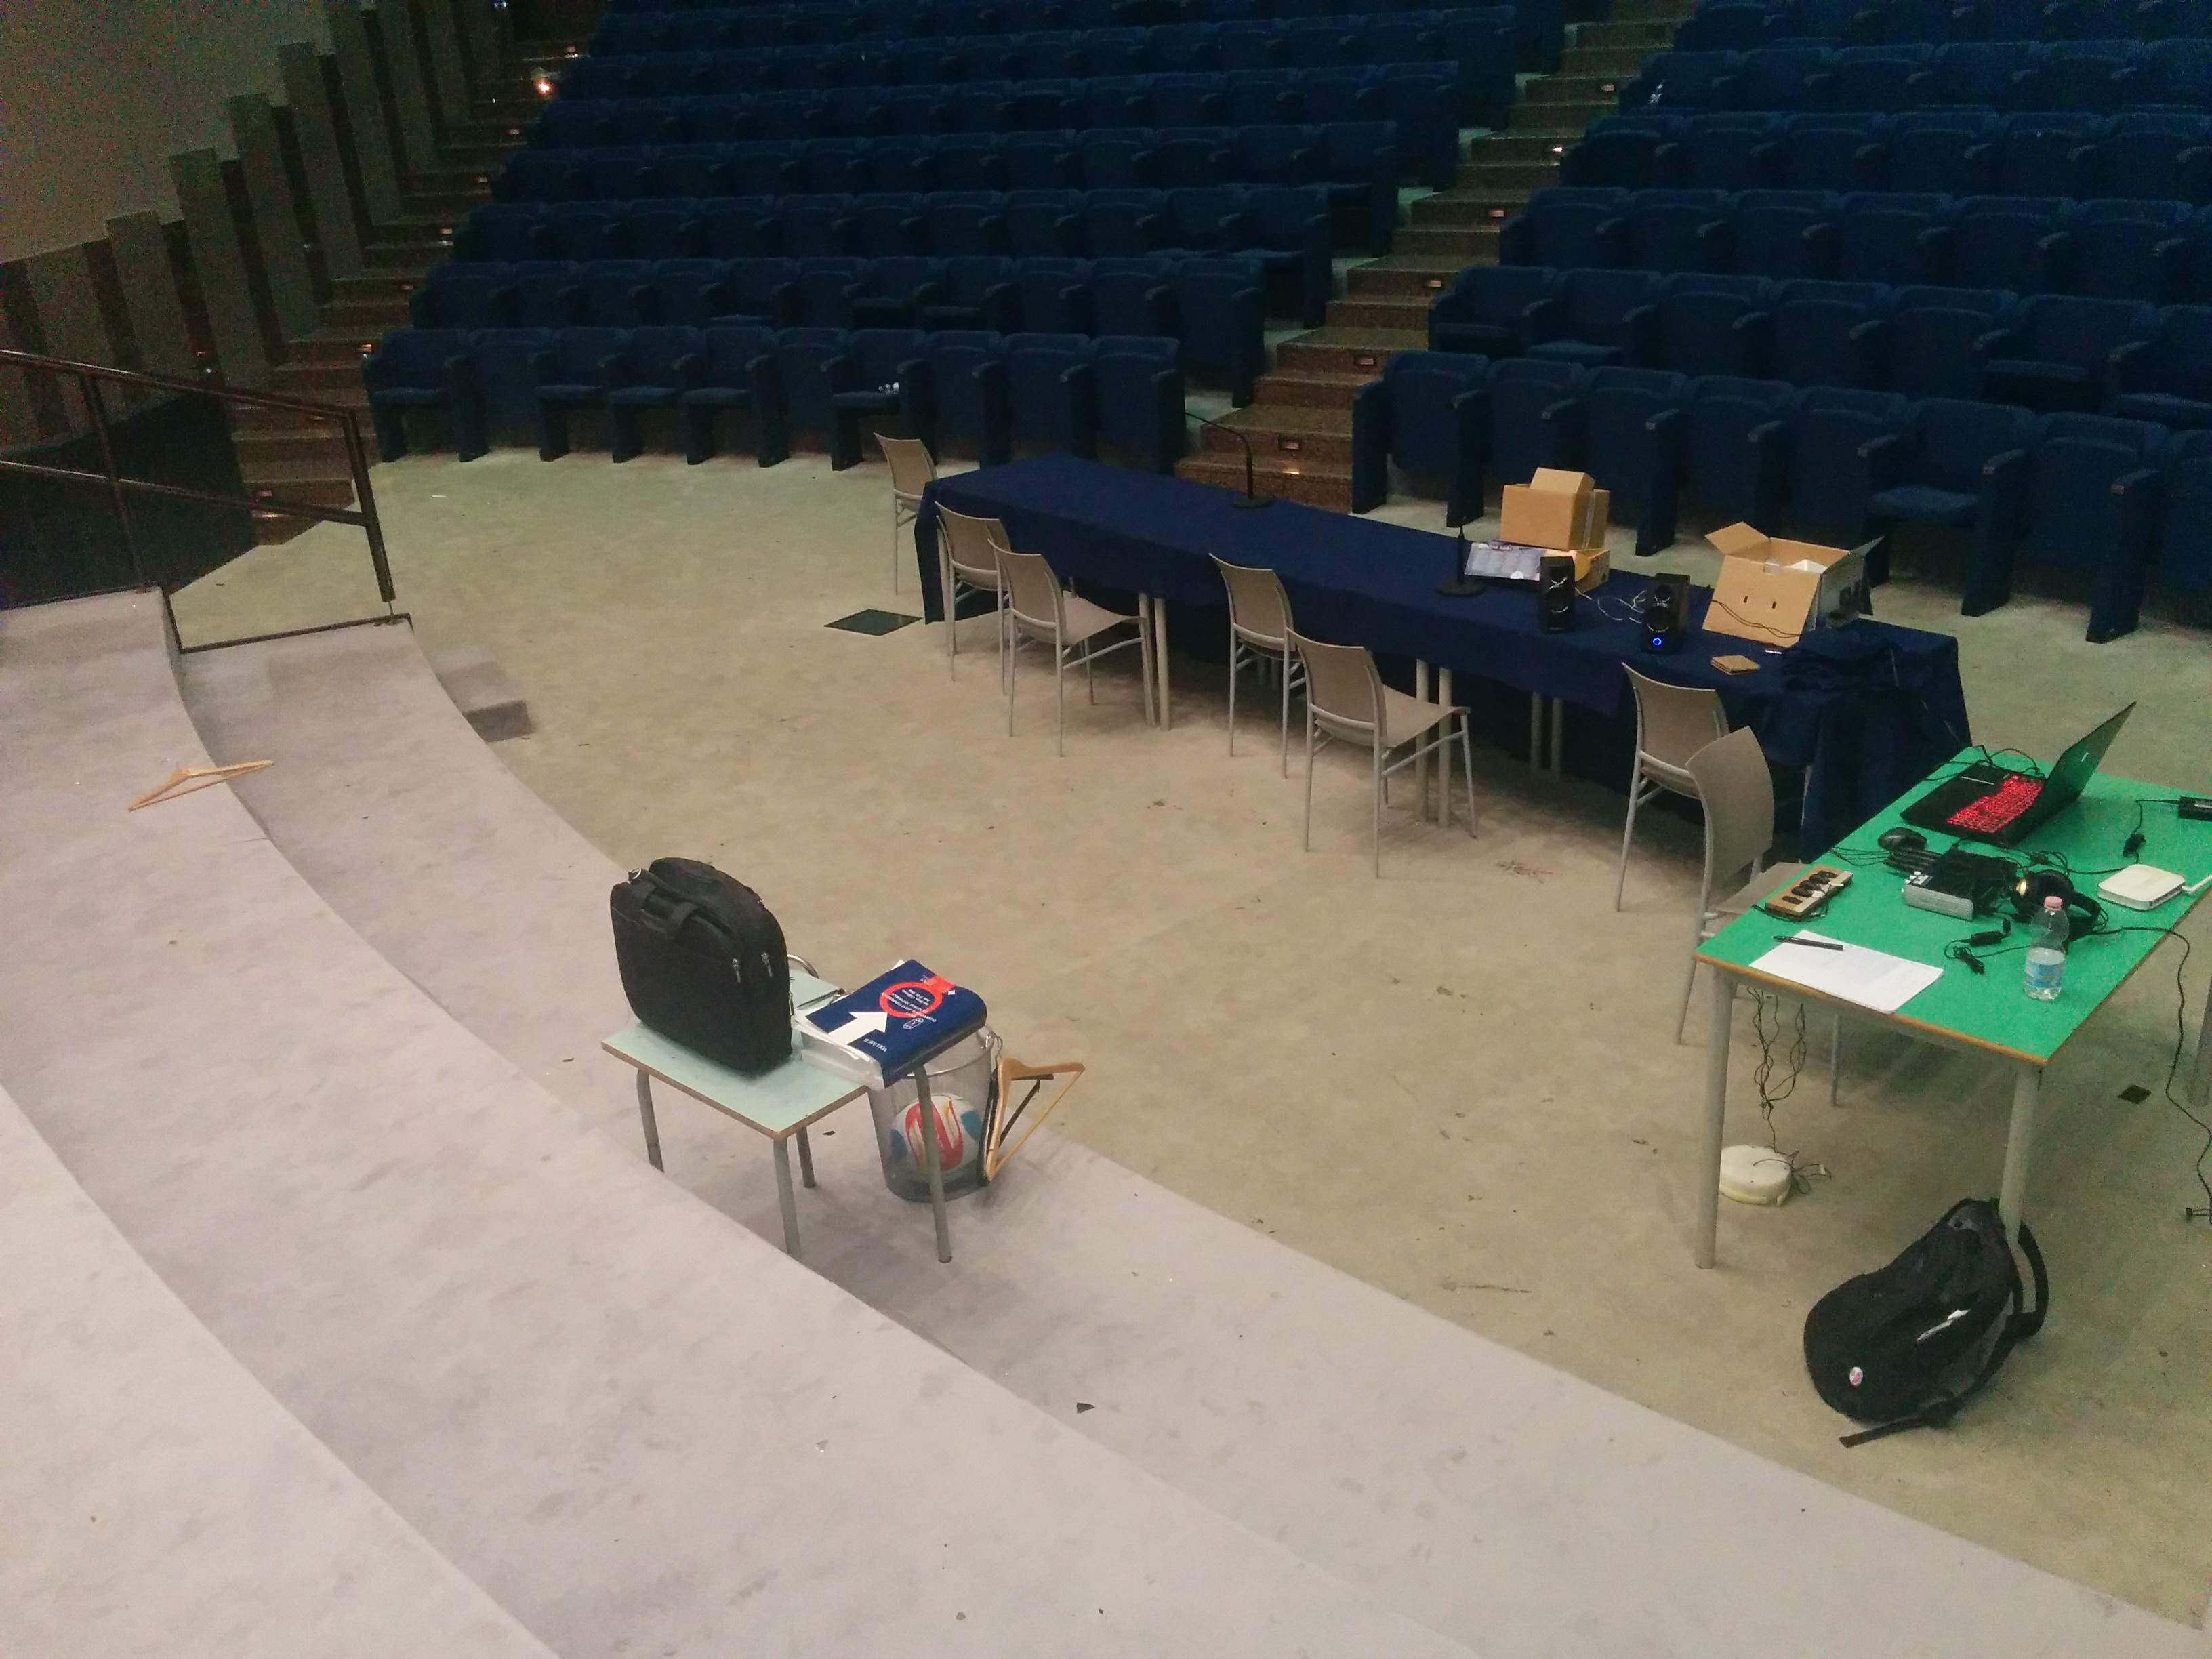
\includegraphics[width=\columnwidth]{img/aula_magna}
	\caption{The auditorium (R0): the fall events were carried out in front of the desk, under the stage, within 6 meters.}
	\label{fig:room1}
\end{figure}

\begin{figure}[htb]
	\centering
	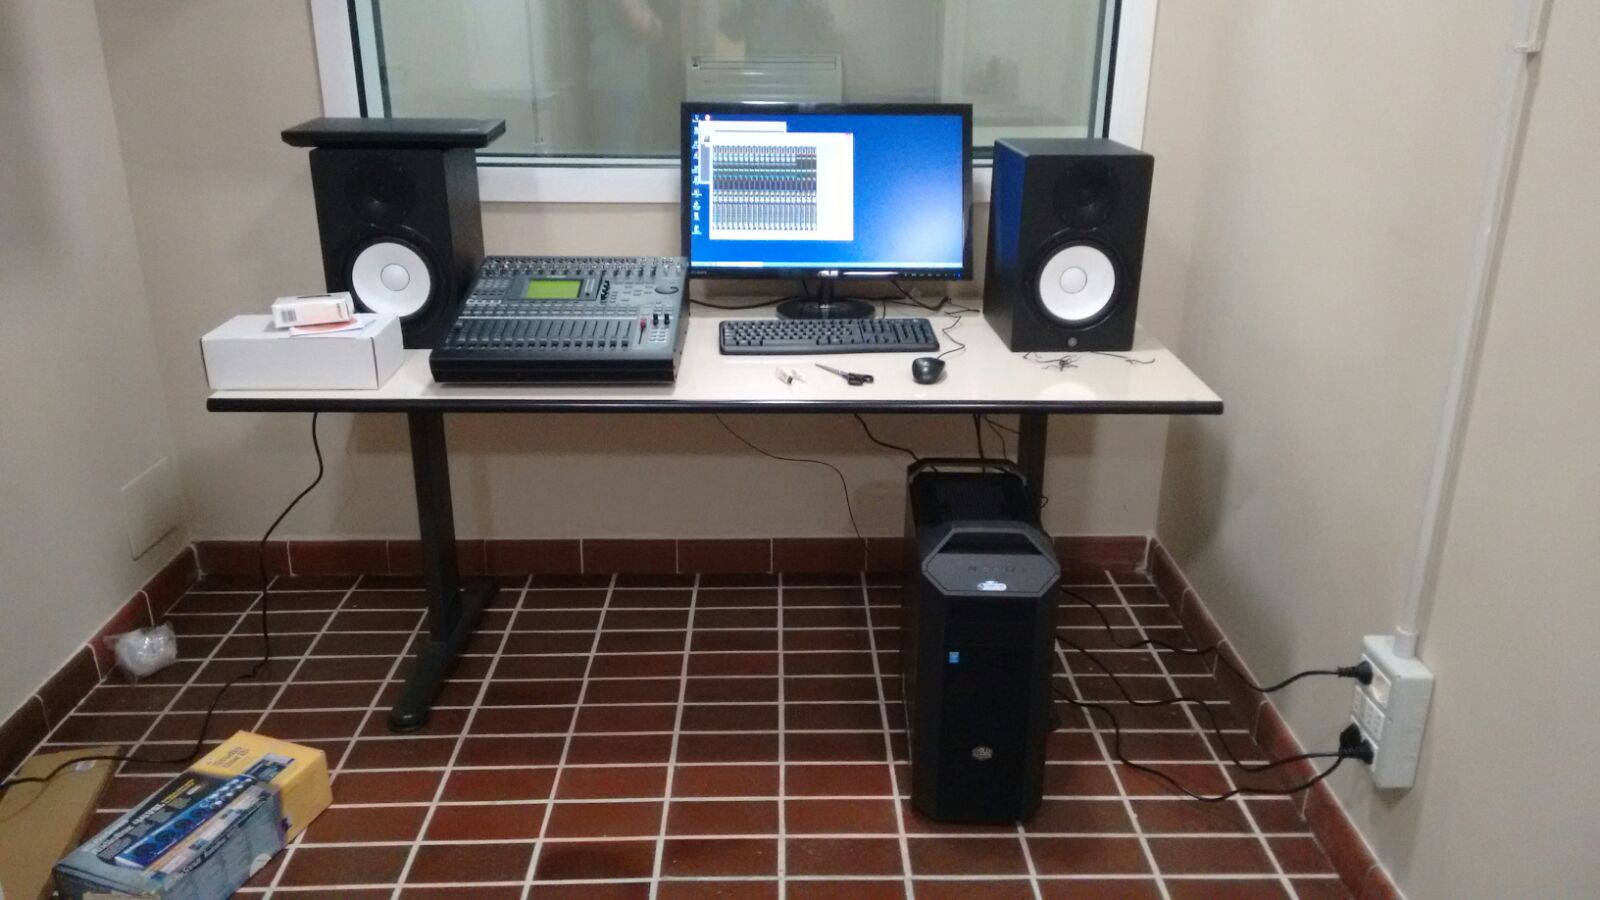
\includegraphics[width=\columnwidth]{img/lolastudio}
	\caption{The studio room (R2) of the LOw Latency LAboratory (LOLA): the fall events were carried out in front of the desk, while the sensors were placed beyond the windows, in the recording room.}
	\label{fig:room2}
\end{figure}
\subsection{Description}
In \tableref{tab:numDataset} the composition of the dataset is summarized.
For the R0, the dataset comprises recordings of fall events related to everyday objects and to a human mimicking doll. The objects were chosen according to the recent literature on the topic \cite{alwan2006smart} and are the following: a ball, a metal basket, a book, a metal fork, a plastic chair, and a bag (\figref{fig:objects}). Objects have been dropped at four distances from the sensors, i.e., 1\,m, 2\,m, 4\,m, and 6\,m, and with various angles in order to reproduce realistically different fall patterns. With the exception of the chair and the basket, which have been overturned from their natural position, half of the falls has been performed at a height of 0.5\,m and the other half at 1\,m. For each object and for each distance, 16 fall events have been performed for a total of 64 events per object. Instead, the chair has been overturned 8 times for each side of fall (back, front, side) and for each distance, thus obtaining a total of 96 events.

\begin{table}[t]
	\caption{Composition of the A3Fall-v2.0 dataset.}
	\label{tab:numDataset}
	\begin{center}
		\begin{tabular}[t]{c|ccc}
			
			\hline
			\textbf{Class} & \textbf{R0} & \textbf{R1} & \textbf{R2} \\ %\cline{2-5} 
			%& \hspace{8pt}Clean\hspace{8pt}  & \hspace{6pt}Clean\hspace{6pt}   \\ 
			\hline
			&\multicolumn{3}{c}{Nr. of occurrences}\\
			Basket      			& 64    &   40 	&   40    	\\
			Fork        			& 64    &   40 	&   40     	\\
			Ball       				& 64    &   40	&   40    	\\
			Book        			& 64    &   40	&   40    	\\
			Bag         			& 64    &   30 	&   40    	\\
			Chair       			& 96    &   40 	&   40    	\\
			Table       			& 0   	&   40 	&   40    	\\
			Guitar Slide       		& 0   	&   40 	&   40    	\\
			Nipper       			& 0    	&   40 	&   40    	\\
			Keys       				& 0    	&   40 	&   40    	\\
			Hook       				& 0    	&   40 	&   40    	\\
			Coat Hook       		& 0    	&   40 	&   40    	\\
			$\,$ Manikin Doll $\,$ 	& 44    &   0 	&   0    	\\
			$\,$ Human Fall $\,$ 	& 0    	&   40 	&   40    	\\
			\hline
			&\multicolumn{3}{c}{Total length (s)}\\			
			%			Human Activity  		& 1135  &   3050&   580   	\\
			%			Music					& 1395  &	4330&   3345  	\\
			%			Television				& 0   	&	1675&   1625  	\\
			Background  			& 2530  &   9055&   5550   	\\
			\hline
		\end{tabular}
	\end{center}
\end{table}

\begin{figure}[htb]
	\centering
	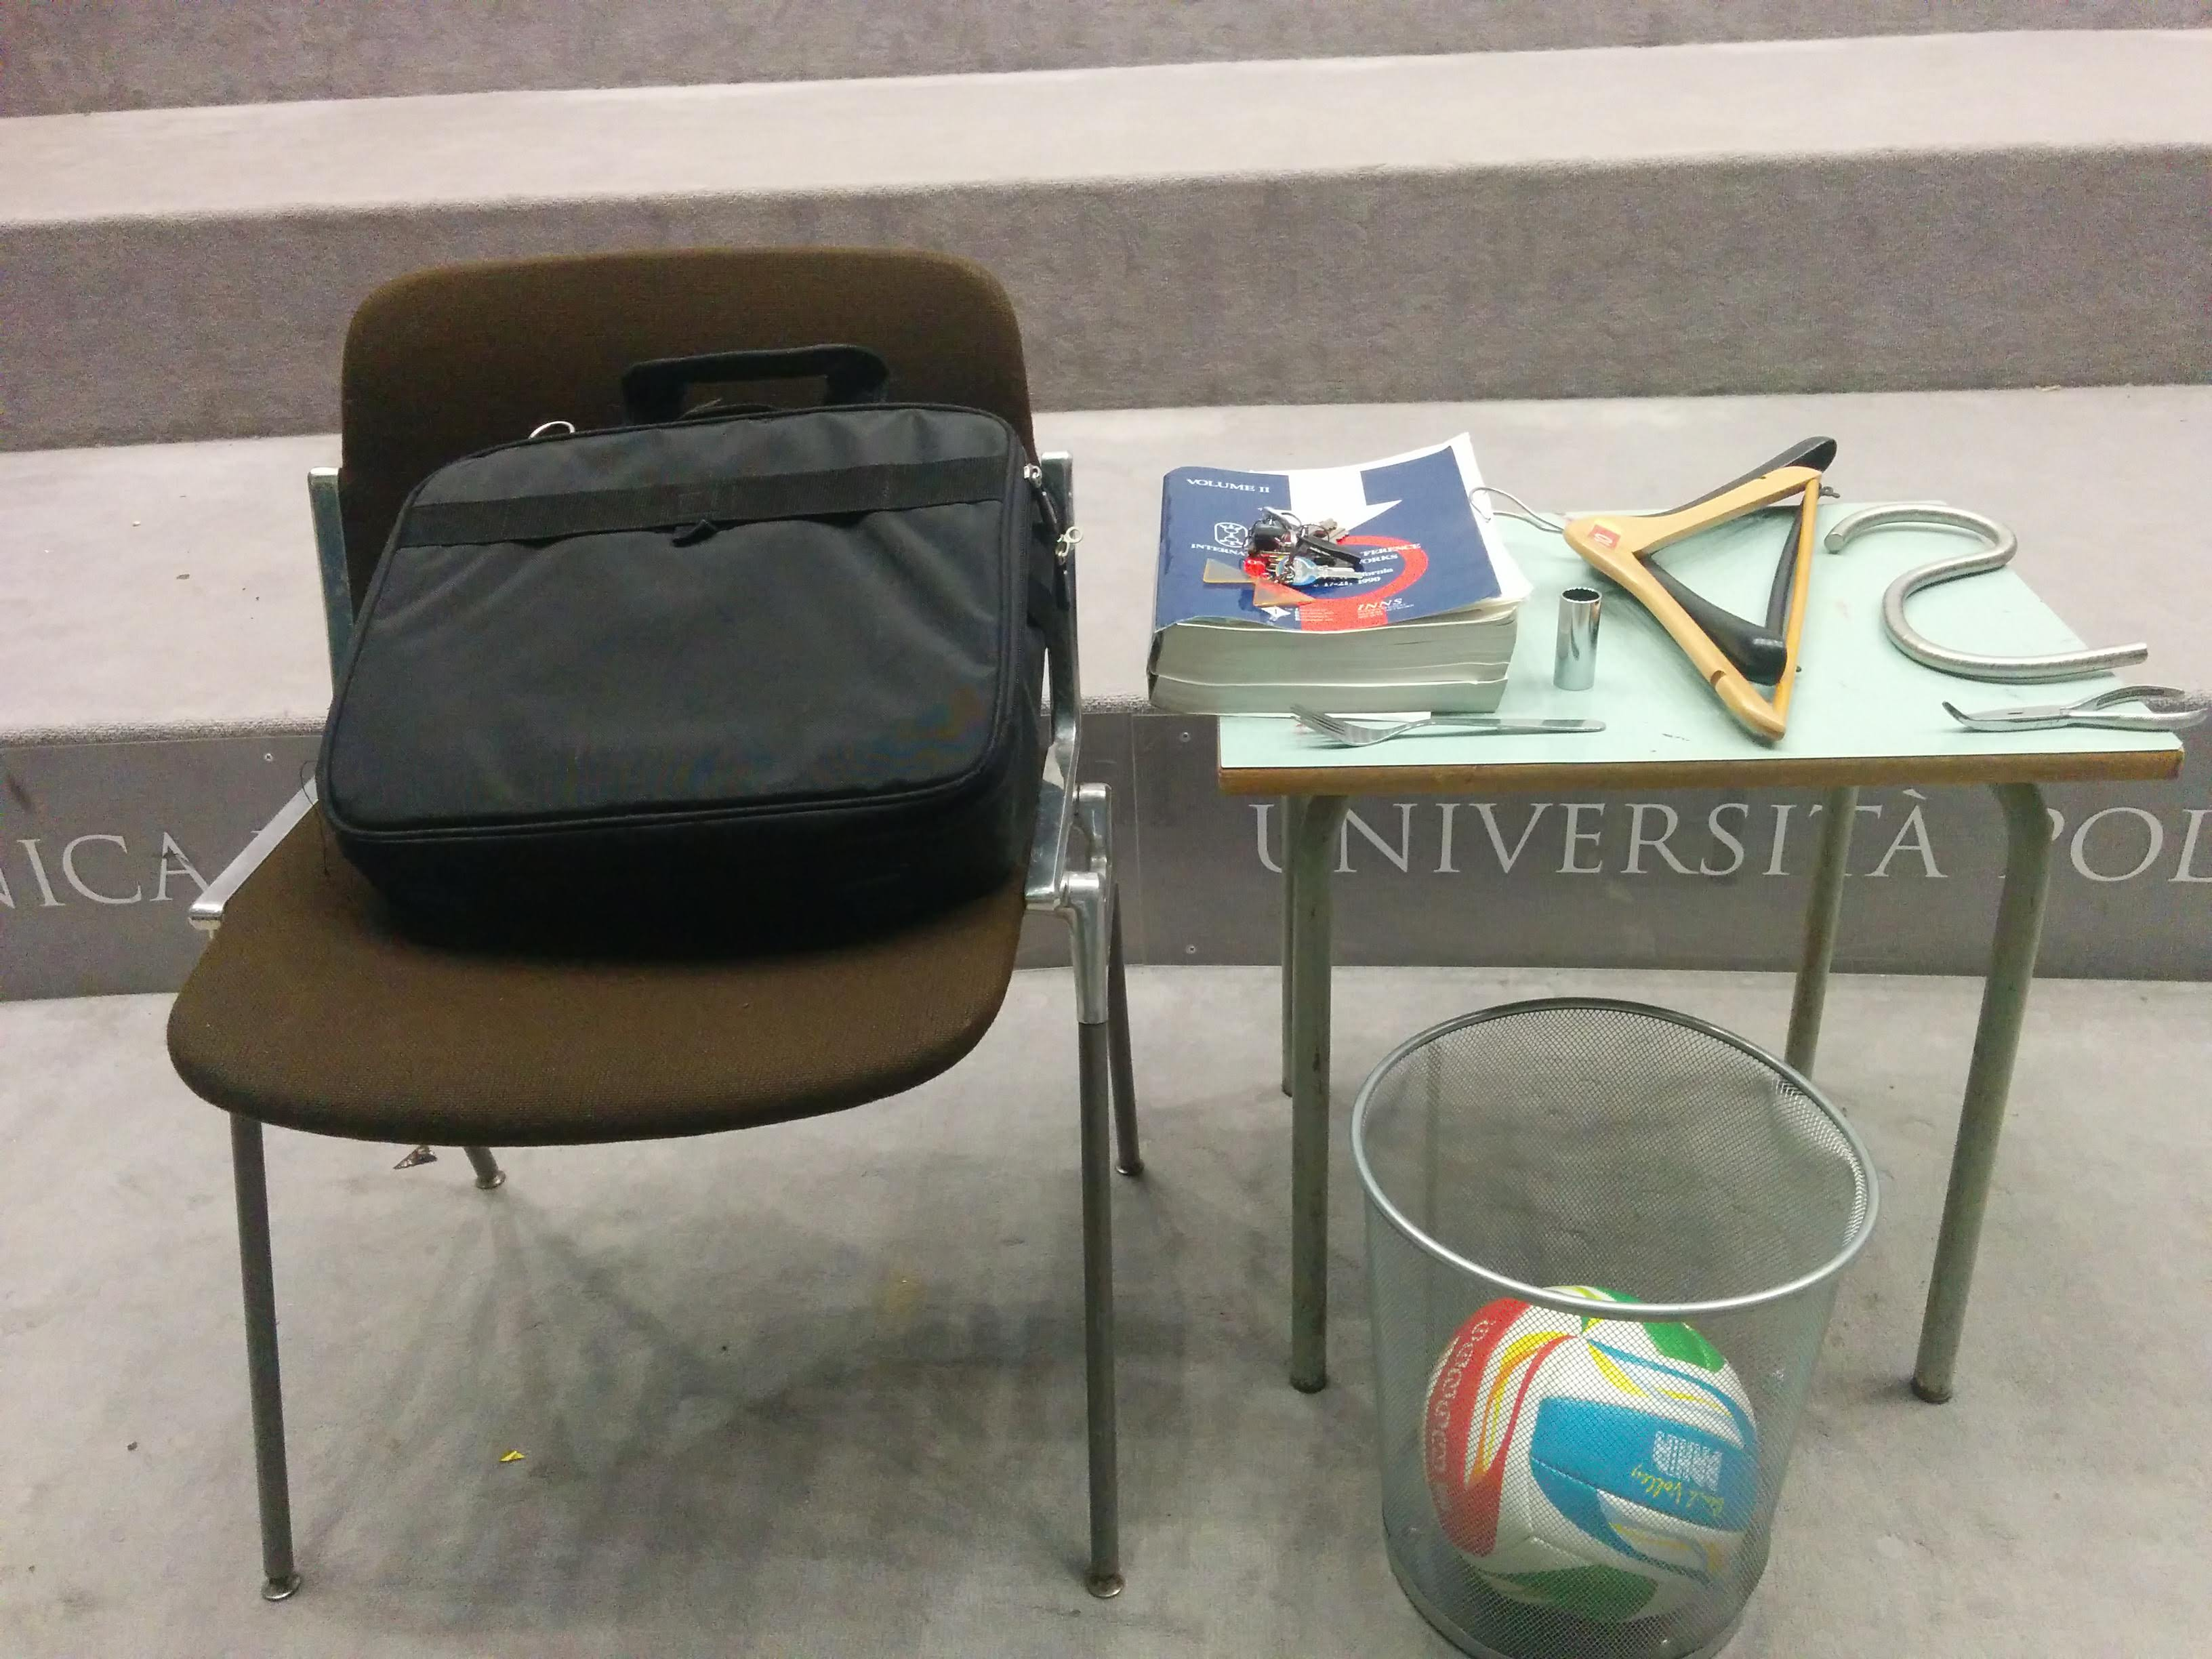
\includegraphics[width=\textwidth]{img/objects_R1_R2.jpg}
	\caption{Objects employed for creating the fall events dataset.}\label{fig:objects}
\end{figure}

Human falls have been simulated by employing the ``Rescue Randy'' doll\footnote{http://www.simulaids.com/1475.htm}, a professional equipment employed in water rescues. It weights 75\,kg, it is 1.85\,m high, and it is equipped with articulated joints. The doll is made of vinyl and its weight is distributed according to the human weight distribution chart. The doll has been dropped from upright position and from a chair, both forward and backward, for a total of 44 events (\figref{fig:randy}). Differently from the everyday objects, the distribution of the fall events with the distance is not uniform: 10 events have been performed from 2\,m, 18 from 4\,m (7 of which from the chair), and 16 from 6\,m (6 of which from the chair).

Moreover, several backgrounds sounds has been added to the dataset. 
Normal activities sounds have been recorded while persons were performing common actions, such as walking, talking, and dragging chairs. Three musical tracks have been played from a loudspeaker and acquired back with the FAS. The first track contained classical music\footnote{W. A. Mozart, ``Piano trio in C major''}, while the second\footnote{Led Zeppelin, ``Dazed and confused''} and the third\footnote{Led Zeppelin, ``When the levee breaks''} rock music. Musical tracks and normal activities sounds have been divided in segments whose lengths have mean and standard deviation estimated from instances of fall events. In addition, they have been employed alone and to create noisy versions of human and object falls occurrences in order to assess the algorithm in presence of interferences. 

In R2 and R1 other every-days objects,in addition to those used in R0, have been recorded for a total of 12 different object fall classes and 1420 instances. While the manikin doll has been used only in R0, in R1 and R2 a total 80 human falls have been performed by 4 people. These falls were performed in different ways: forward, backward and on the side, trying to use the arms to cushion the fall and without any protections. As in R0, also in R2 and R2 all events were performed from 1, 2, 4 and 6 m away from the FAS.

\begin{figure}[htb]
	\centering
	\begin{subfigure}[b]{0.48\textwidth}
		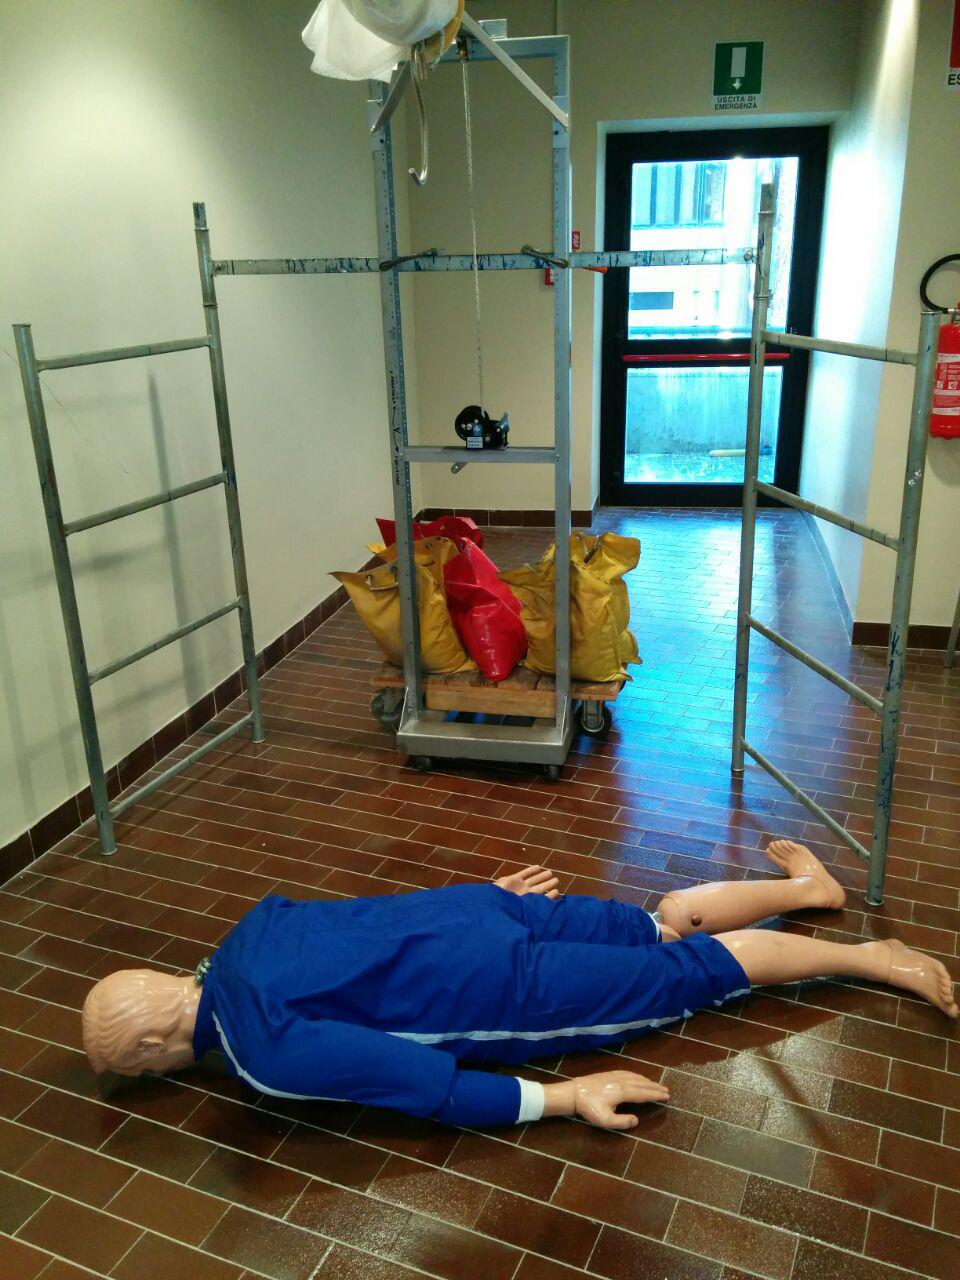
\includegraphics[width=\textwidth]{img/impalcatura.jpg}
		\caption{Fall from upright position.}\label{fig:randy_upright}
	\end{subfigure}
	\begin{subfigure}[b]{0.48\textwidth}
		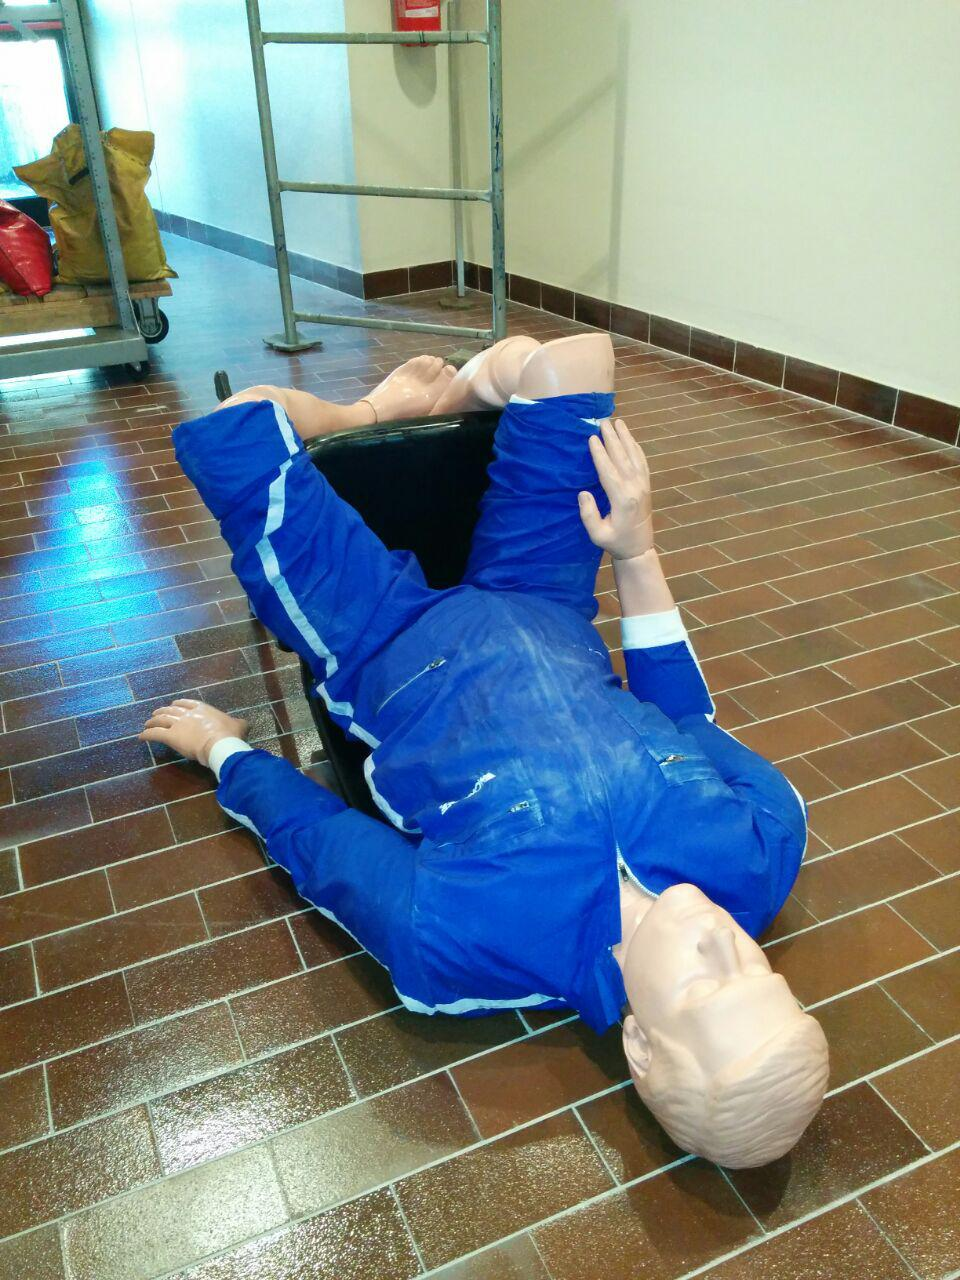
\includegraphics[width=\textwidth]{img/rndy_caduta_sedia.jpg}
		\caption{Fall from the chair.}\label{fig:randy_chair}
	\end{subfigure}
	\caption{Falls of the ``Rescue Randy'' doll from upright position (a) and from the chair (b). carried out in the R0 room}\label{fig:randy}
\end{figure}



As shown in \tableref{tab:numDataset} background noises have been recorded also in R1 and R2 rooms rooms, which include: human activities noise as, i.e., footsteps, human and phone conversation, dragging objects and so on; classic, rock and pop music played from loudspeakers; TV shows like newscast and satiric.

Since the data relating to rooms R1 and R2 have been collected at different times to those of room R0, in the following chapters, for each proposed approach, it will be specified which subset of the total dataset has been used as well as the usage of the noisy version of falls events.


\subsection{Signal analysis}\label{ssec:sig_analysis}
The signal related to the same fall event acquired with the floor sensor and with the aerial microphone exhibits different spectral characteristics. In this section and in depth analysis of the audio signals acquired in the R0 room is presented. \figref{fig:spectrograms} shows the spectrograms of a doll fall acquired with the floor sensor (above) and with the aerial microphone (below) in the clean acoustic condition. Observing the figures, it can be noticed that the aerial microphone is more sensitive to high frequencies, in particular to the ones above 1.5\,kHz. On the contrary, the majority of the energy of the signal acquired with the floor sensor concentrates below 1\,kHz. 

This is even more evident by plotting the values of the mel coefficients (\figref{fig:mel}): the first and second mel channels of the FAS, corresponding to the frequency bands 0--128.10\,Hz and 61.30-200.60\,Hz, are higher respect to the aerial microphone. Channels 3 to 7, respectively corresponding to bands 128.10--279.50\,Hz and 458.70--670.70\,Hz, are almost equivalent, while from channel 8 (560.30--790.80\,Hz) to 29 (6654.60--8000.00\,kHz) the aerial microphone mels are greater.

\begin{figure}[htb]
	\centering
	\begin{subfigure}[b]{0.9\textwidth}
		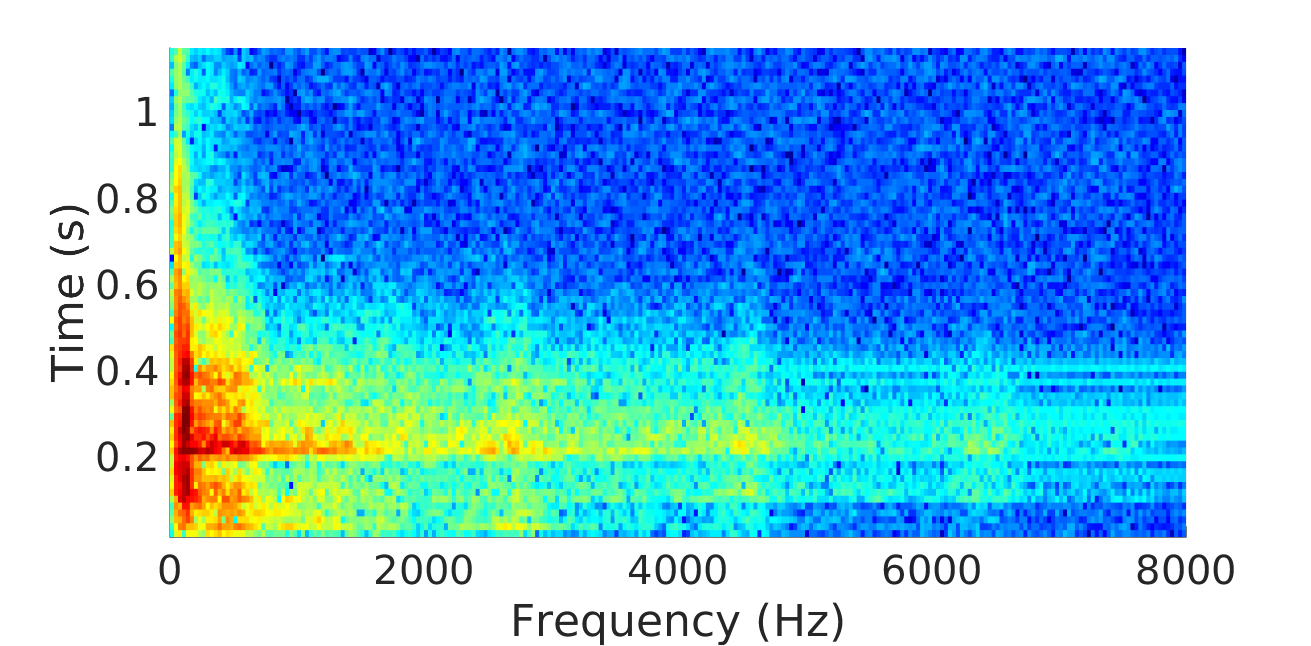
\includegraphics[width=\textwidth]{img/spettro_fas}
		\caption{Spectrogram of the signal acquired with the floor sensor.}
		\label{fig:spec_fas}
	\end{subfigure}
	\begin{subfigure}[b]{0.9\textwidth}
		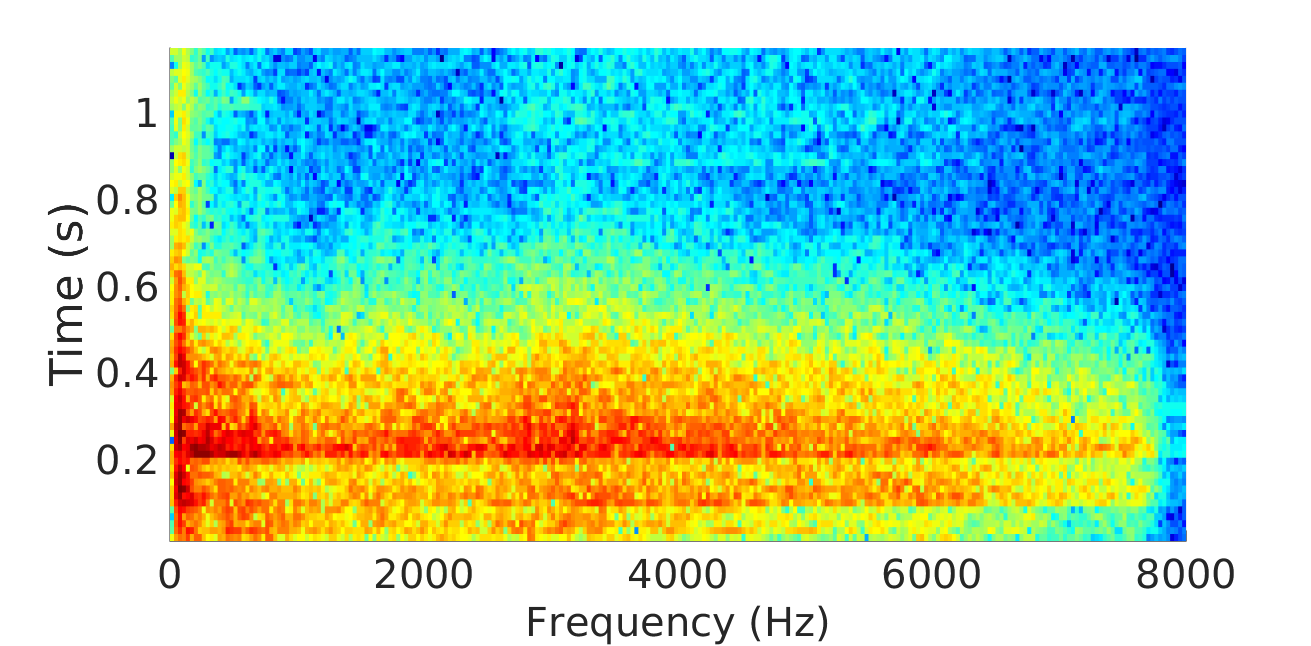
\includegraphics[width=\textwidth]{img/spettro_mic}
		\caption{Spectrogram of the signal acquired with the aerial microphone.}
		\label{fig:spec_aer}
	\end{subfigure}
	
	\caption{Frequency content of the same fall event (file ``rndy\_d2st\_bar\_0.wav'') acquired with the FAS (a) and with the aerial microphone (b).}\label{fig:spectrograms}
\end{figure}

\begin{figure}[htb]
	\centering
	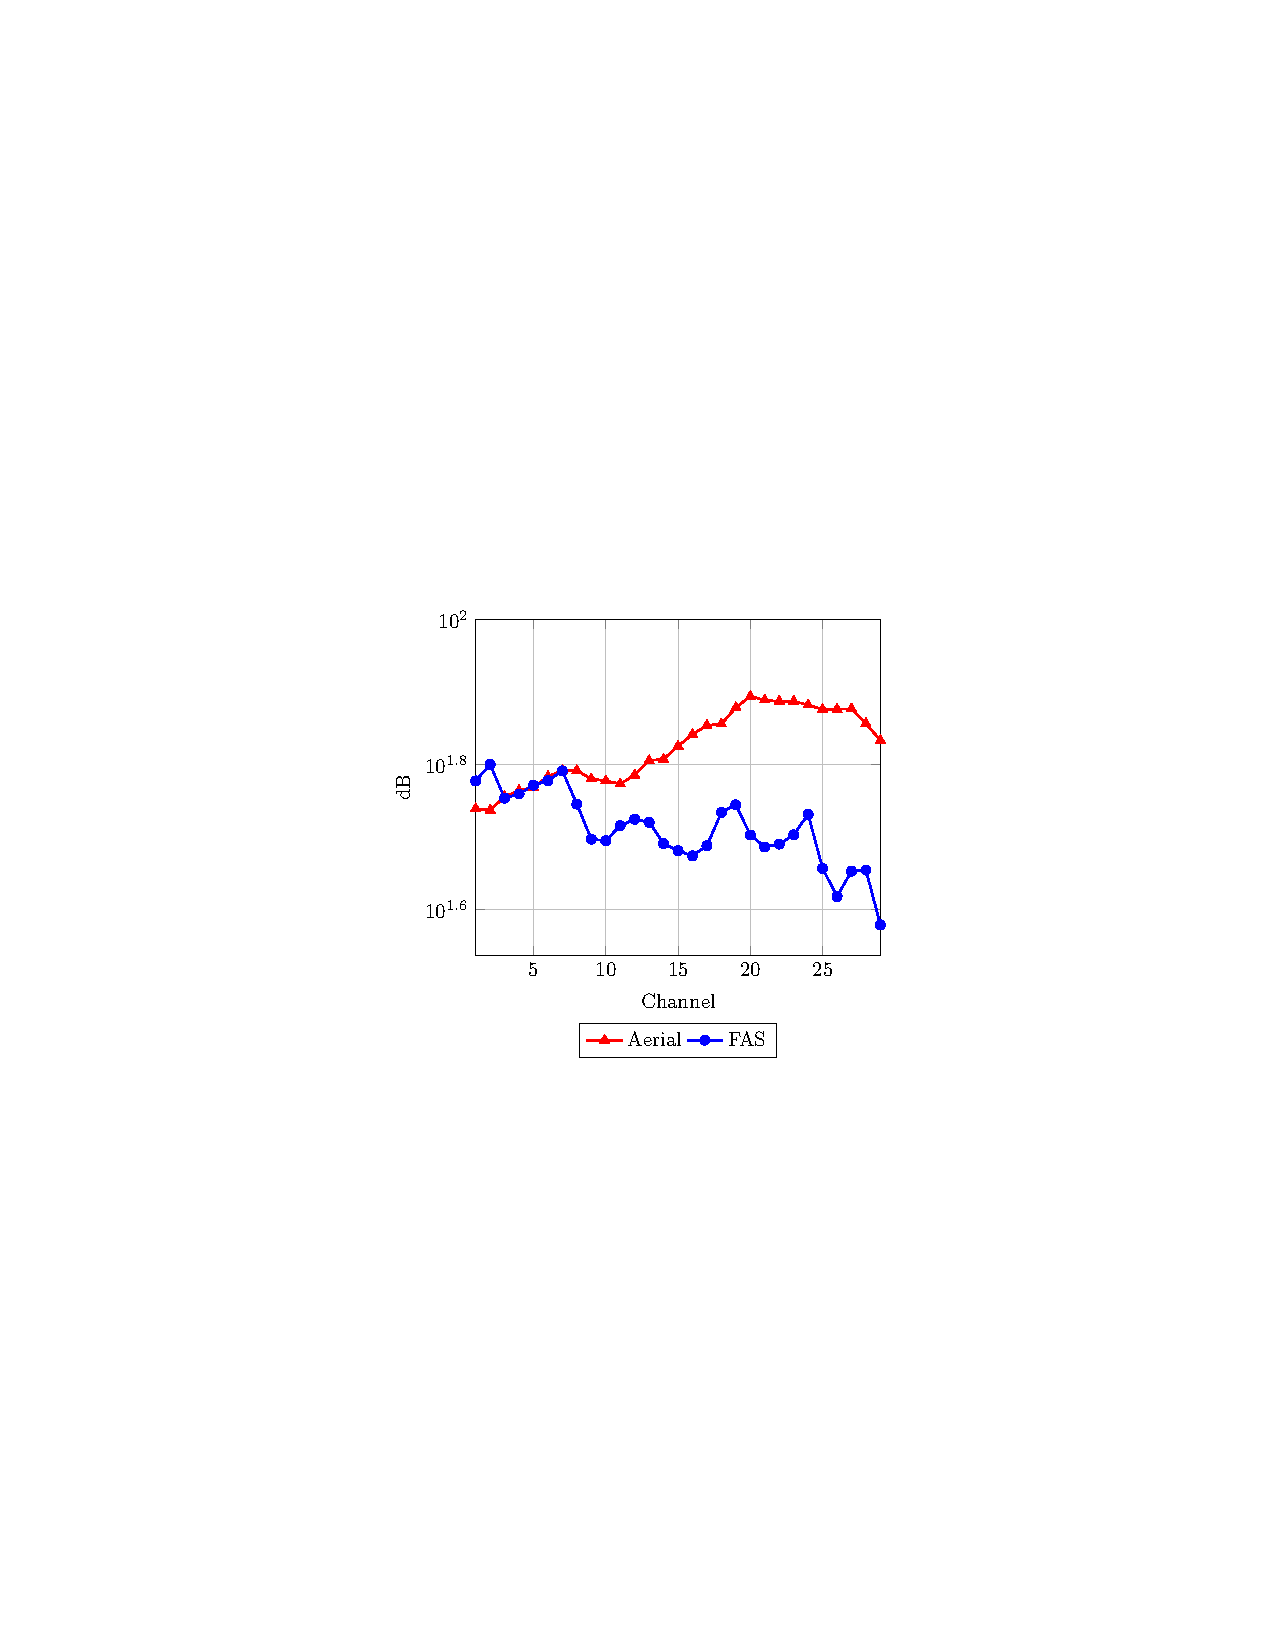
\includegraphics[width=0.75\textwidth]{img/mel_dB}
	\caption{Average value of the mel channels.} \label{fig:mel}
\end{figure}

\begin{figure}[htb]
	\centering
	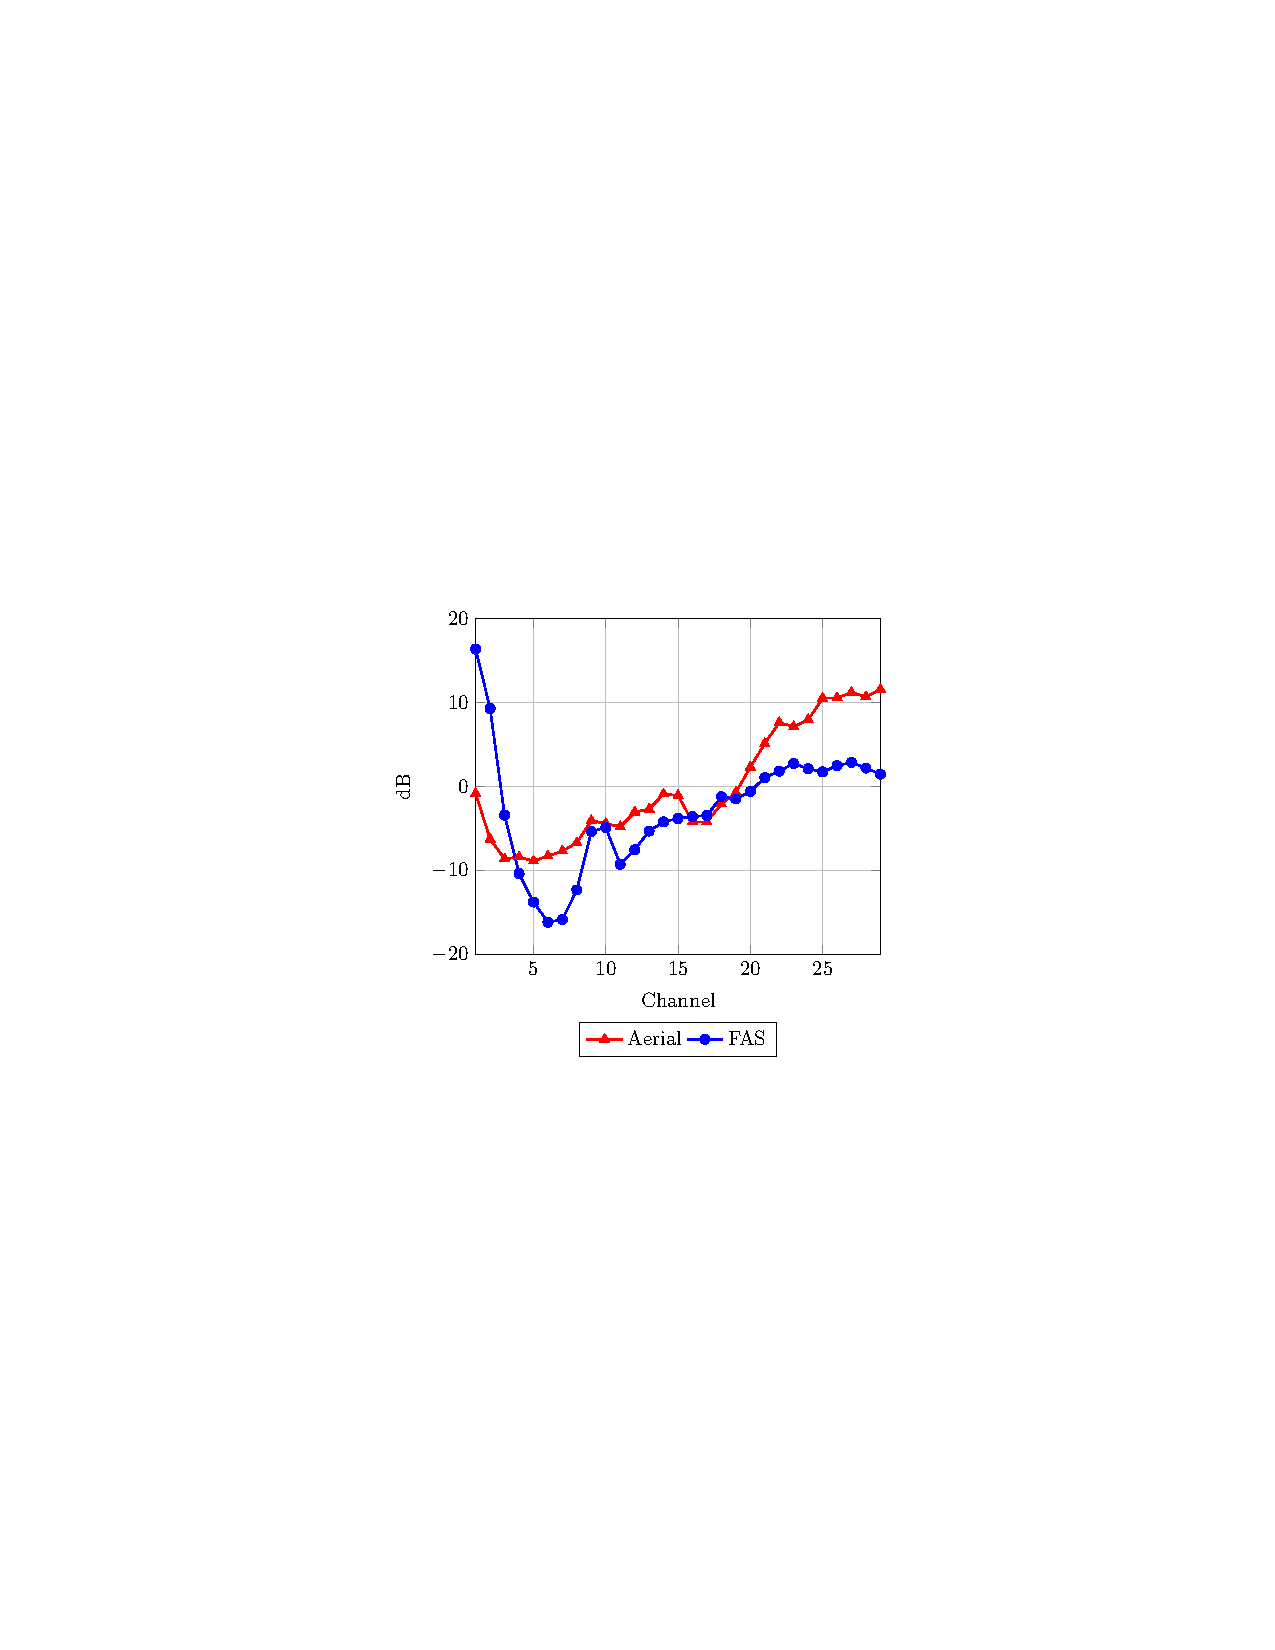
\includegraphics[width=0.75\textwidth]{img/SNR_mel_channel}
	\caption{Average value of the SNR for each mel channel.} \label{fig:noisymel}
\end{figure}

The analysis of noisy signals highlights the different behaviour of the floor sensor respect to the aerial microphone in presence of external interferences. 
In fact, taking into account the backgrounds tracks as interferences, the floor sensor has a global signal-to-noise ratio (SNR) equal to 20.94\,dB and a segmental SNR equal to 7.28\,dB. The global SNR of the central aerial microphone is 8.92\,dB and the segmental SNR is -1.47\,dB. The values of the aerial microphone SNRs are thus considerably lower than the ones of the floor sensor.%: this highlights the superiority of the FAS respect to the aerial microphone in reducing sounds propagating through the air and not related to fall events.
The global SNR of the floor sensor noisy dataset is 13.66\,dB higher than the one of the aerial microphone, highlighting the superior ability of the former to isolate fall signals from external interferences. However, it is worth investigating how the SNR distributes over the frequency range of the acquired signals in order to have a better insight of the physical phenomenon. \figref{fig:noisymel} shows the SNR calculated for each mel channel and averaged across the noisy datasets. It can be noticed that the SNR of the floor sensor exceeds the one of the aerial microphone for channels below the fourth. Then, the opposite occurs and the SNR of the aerial microphone assumes greater values. The ``valley'' in the curves are due to the pitch of the music signal.




\graphicspath{{4_Supervised_approaches/}}
\chapter{Supervised Approach}
qua vengono presentati sia il metodo multilabel classifier GMM-UBM SVM (ESWN) che 
il binary  GMM-UBM SVM (WIRN2016)



\graphicspath{{5_Unsupervised_approaches/}}
\chapter{Unsupervised Approach}
\label{ch:unsupervised_approaches}

The problem with supervised approaches is that they require that each class of interest is well represented in the training dataset. However, in some case the variability of the environmental conditions or the subjects makes difficult or impossible to collect a sufficient number of examples that allow the algorithm to generalize well on unseen conditions \cite{Noury2007}. This is the case of human falls. Unsupervised approaches tackle the problem as a novelty detection task \cite{markou2003novelty1,markou2003novelty2}, i.e., by learning a normality model from data not related to human falls. In this chapter two approaches are proposed. The fist (\secref{sec:ocsvm_approach}) in based on One-Class SVM \secref{sec:ocsvm_theory} trained with only background noises. The second \secref{sec:autoencoder} instead, approaches the problem from an end-to-end learning prospective by means of neural network autoencoder \secref{sec:autoencoder_theory} for novelty detection.

Since the previous results have shown the superiority of the FAS with respect to the standard microphone, in the next sections only the samples recorded with the FAS has been used, unless otherwise specified.

\section{One-Class Support Vector Machine based algorithm}
\label{sec:ocsvm_approach}

The approach proposed in this section is based on a One-Class Support Vector Machine (OCSVM) \cite{scholkopf2000} to obtain an unsupervised framework for Fall Detection.
The acoustic signals are captured by means the Floor Acoustic Sensor and then MFCCs and Gaussian Mean Supervectors (GMSs) are extracted by using the same methods described in \secref{sec:svm_multi_classification}: GMSs are higher level features computed by adapting the means of a Gaussian mixture model (GMM) with maximum a posteriori algorithm (MAP).
In the training phase, a large set of audio data is used to model an Universal Background Model (UBM) composed of the GMM extracted by using Expectation Maximization (EM) algorithm \cite{bilmes1998gentle}.
Then, the GMS of each event is calculated by adapting the GMM with the MAP algorithm and concatenating the resulting GMM mean values.
Abnormal acoustic events are discriminate from normal ones employing the OCSVM classifier.


\subsection{Data Used}
\label{sec:dataset_cin_ocsvm_only}
The performance of the algorithm has been evaluated on a corpus containing sounds of human falls, falling objects, human activities, and music. In particular, from the dataset presented in \secref{sec:dataset}, have been used the samples reported in \tableref{tab:ocsvm_dataset}.

\begin{table}[t]
	\caption{Composition  of the dataset.}
	\label{tab:ocsvm_dataset}
	\begin{center}
		\begin{tabular}[t]{c>{\centering}m{5cm}c}
			
			\hline
			\textbf{Class} & \textbf{Nr. of occurrences} & \textbf{Total length (s)} \\ %\cline{2-5} 
			%& \hspace{8pt}Clean\hspace{8pt}  & \hspace{6pt}Clean\hspace{6pt}   \\ 
			\hline
			Basket      			& 64    &   86    \\
			Fork        			& 64    &   82     \\
			Ball       				& 64    &   129     \\
			Book        			& 64    &   63    \\
			Bag         			& 64    &   57     \\
			Chair       			& 96    &   157     \\
			$\,$ Human Falls $\,$ 	& 44    &   76     \\
			Human Activity  		& 665   &   1218     \\
			Music					& 776   &	1498	\\
			%				 Classic Music       	& 441   &   882     \\
			%				 Rock Music       		& 335   &   616     \\
			\hline
		\end{tabular}
	\end{center}
\end{table}

Musical tracks and normal activities sounds have been divided in segments whose lengths have mean and standard deviation estimated from instances of fall events. In addition, they have been employed alone and to create noisy versions of human and object falls occurrences in order to assess the algorithm in presence of interferences.

In the experiments, signals have been downsampled to 8\,kHz and the resolution has been reduced to 16\,bit. As in the approach presented previously, the choice of the sampling frequency is motivated by the analysis performed in a previous work by the authors \secref{ssec:sig_analysis}, where it was shown that the signals recorded with the FAS have the majority of the energy concentrated at frequencies below 1\,kHz.

\subsection{Experimental setup}
\label{sec:experiment_ocsvm}
The dataset described previously has been divided in one set for training the UBM and the OCSVM and three sets for evaluating the performance.

Training has been performed on the set shown in \tableref{tab:trainComposition} composed of 947 occurrences (1773\,s) of human activities, classical music and rock music. The assessment of the algorithm has been performed on the following datasets:
\begin{itemize}
	\item Set 1 (Human fall and background sounds): this set comprises 44 examples of human fall sounds and 44 examples of human activity and music sounds (\tableref{tab:set1Composition}).
	\item Set 2 (Human fall and object fall sounds): this set comprises 44 examples of human fall sounds and 44 examples of object fall sounds (\tableref{tab:set2Composition}).
	\item Set 3 (Human fall, object fall and background sounds): this set comprises 44 examples of human fall sounds, 22 examples of background sounds and 22 examples of object fall sounds (\tableref{tab:set3Composition}).
\end{itemize}



\begin{table}[t]
	\caption{Composition  of the training-set.}
	\label{tab:trainComposition}
	\begin{center}
		\begin{tabular}{c>{\centering}m{5cm}c}			
			\hline
			\textbf{Class} & \textbf{Nr.\ of occurrences}  & \textbf{Total length (s)} \\ 
			\hline
			Human Activity  		& 320 &  593		\\
			Music					& 627 &  1180       \\
			%			 Classic Music       	& 306 &  591		\\
			%			 Rock Music       		& 321 &  589 	 	\\
			\hline
			Total                 & 947 & 1773 \\
			\hline
		\end{tabular}		
	\end{center}
\end{table}

\begin{table}[t]
	\centering

	\caption{Composition  of ``Set 1''.}
	\label{tab:set1Composition} % è lo stesso del capitolo 6
	\begin{center}
		\begin{tabular}{K{3cm}K{3cm}}				
			\hline
			\textbf{Class} & \textbf{Nr.\ of occurrences} \\ 
			\hline
			$\,$ Human Falls $\,$ 	& 44    			\\
			Human Activity  		& 15		\\
			Music			  		& 29		\\
			%				 Classic Music       	& 15   		\\
			%				 Rock Music       		& 14  		\\		
			\hline
		\end{tabular}			
	\end{center}		

\end{table}

\begin{table}[t]
	\centering
		
	\caption{Composition  of ``Set 2''.}
	\label{tab:set2Composition}
	\begin{center}
		
		\begin{tabular}{K{3cm}K{3cm}}
			
			\hline
			\textbf{Class} & \textbf{Nr. of occurrences} \\ 
			%& \hspace{8pt}Clean\hspace{8pt}  & \hspace{6pt}Clean\hspace{6pt}   \\ 
			\hline
			$\,$ Human Falls $\,$ 	& 44    		\\				
			Basket      			& 7           	 \\
			Fork        			& 7           	 \\
			Ball       			& 8           	 \\
			Book        			& 7          	  \\
			Bag         			& 8          	  \\
			Chair       			& 7    			\\
			
			\hline
		\end{tabular}
		
	\end{center}
	
\end{table}


\begin{table}[t]
	
	\caption{Composition  of ``Set 3''.}
	\label{tab:set3Composition}
	\begin{center}
		
		\begin{tabular}{K{3cm}K{3cm}}
			
			\hline
			\textbf{Class} & \textbf{Nr. of occurrences} \\ 

			\hline
			$\,$ Human Falls $\,$ 	& 44    		\\				
			Basket      			& 3            	\\
			Fork        			& 4            	\\
			Ball       			& 4            	\\
			Book        			& 3            	\\
			Bag         			& 4            	\\
			Chair       			& 4    			\\
			Human Activity  		& 8   			\\
			Music			  		& 14   			\\
			%				 Classic Music       	& 7   			\\
			%				 Rock Music       		& 7   			\\
			
			\hline
		\end{tabular}
		
	\end{center}
		
\end{table}

For each set, the data have been divided in four folds, each composed of 11 human falls and 11 non-falls. Then, one fold has been used for estimating the hyperparameters of the algorithm and three for calculating the performance. The final performance is calculated by using the cumulative true positives, false positives, and false negatives obtained by varying the test folds.
The validation phase consisted in searching for the number of components of the UBM, the values of $\nu$ and $\gamma$ of the OCSVM. The values assumed by these variables are summarised in \tableref{tab:parameter_ocsvm}.

\begin{table}[t]
	\centering
	\caption{Hyperparameters of the algorithm and search space explored in the validation phase.}
	\label{tab:parameter_ocsvm}
	\begin{tabular}{c |c | c}
		\hline
		\textbf{Stage} & \textbf{Hyperparameter} & \textbf{Range} \\
		\hline
		UBM & $J$ & $1, 2, 4, \ldots , 64$\\
		\hline
		\multirow{2}{*}{OCSVM} & $\nu$ & $0.1, 02, \ldots, 1.0$ \\
		&$\gamma$ & $2^{-15}, 2^{-13}, \ldots,2^{3} $ \\
		\hline

	\end{tabular}
\end{table}

\paragraph{Comparative method}
\label{par:popescu_mod}
The proposed approach has been compared to the algorithm presented in \cite{Popescu2009} based on OCSVM. The same algorithm has also been employed in \cite{khan2015unsupervised} with a multi-microphone acquisition setup and a source separation stage. As in \cite{Popescu2009}, the audio signals are divided in windows of the same lengths, and the related MFCCs are used for training the OCSVM and for classification. In \cite{Popescu2009}, 7 MFCCs were extracted from audio signals sampled at 20\,kHz and the length of the window was set to 1\,s. Here, the feature vectors are the same of the proposed approach, i.e., they are composed of the first 13 MFCCs and their first and second derivatives. The same window length of \cite{Popescu2009} cannot be employed here, since the dataset used in this paper comprises signals with lengths less than 1\,s. Thus, the length of the window corresponds to the duration of the shortest event in the dataset, and it is equal to 576\,ms (71 frames). Windows are overlapped by 50\%, and, as in \cite{Popescu2009}, an event is classified as fall if at least two consecutive frames are classified as novelty by the OCSVM. The same grid search procedure of the proposed approach has been adopted to search for the optimal values of $\nu$ and $\gamma$ of the OCSVM.


The performance has been evaluated in terms of F$_1$-Measure calculated as:
\begin{equation}
\label{eq:f1}
\text{F}_1\text{-Measure} = \frac{2\cdot tp}{2\cdot tp+fn+fp},
\end{equation}
where $tp$ is the number of correctly classified falls, $fn$ is the number of falls misclassified as non-falls, and $fp$ is the number of non-falls misclassified as falls.


\subsection{Results}
\label{sec:ocsvm_results}
\figref{fig:res_clean} shows the results in clean conditions obtained with the proposed method named ``OCSVM'' and the comparative method proposed in \cite{Popescu2009} denoted as ``Popescu (2009)''. Observing the figure, it is evident that in all the three cases the OCSVM approach is able to improve the performance with respect to ``Popescu (2009)'' \cite{Popescu2009}. In particular, in ``Set 1'', that comprises human falls, human activities and music, the performance improves by 16.73\% with respect to ``Popescu (2009)''. This case can be considered as the least challenging of the three, since non-falls events are considerably different from falls ones. Conversely, ``Set 2'' comprises both human falls and object falls, thus it includes abnormal events whose pattern is similar to the one of human falls. Indeed, the performance with respect to ``Set 1'' is 17.91\% lower, mostly due the increased false positives rate that goes from 13.64\% to 50.76\%. Regarding ``Popescu (2009)'' \cite{Popescu2009}, the F$_1$-Measure is below both OCSVM and the proposed approach, however it is less affected by the presence of object falls, since the F$_1$-Measure decreases only by 0.64\% . ``Set 3'' comprises human falls, human activities, music and object falls and represents the most realistic test condition of the three. The results obtained by using  the OCSVM classifier alone is 82.25\%. As expected, this result is lower than ``Set 1'', since object falls are also present, and higher than ``Set 2'', since human activities and music segments are easier to discriminate.  Differently, the approach by Popescu and Mahnot \cite{Popescu2009} degrades by 5.25\% with respect to ``Set 1'', and by 4.61\% with respect to ``Set 2'', demonstrating that it is less robust to the concurrent presence of object falls and daily human activities sounds. 

\begin{figure}[htb]
	\centering
	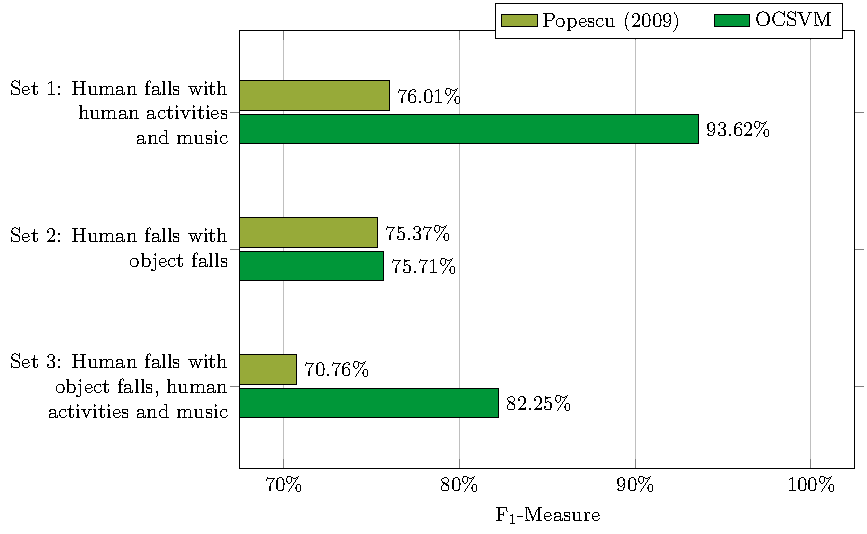
\includegraphics[width=\columnwidth]{img/cin_only_ocsv/res_clean.pdf}
	\caption{Results in \textit{clean} conditions for the three test cases. ``Set 1'' comprises human falls, human activities and music. ``Set 2'' comprises human falls and object falls. ``Set 3'' comprises human falls, object falls, human activities, and music.} \label{fig:res_clean}
\end{figure}

\figref{fig:res_noisy} shows the results obtained for the three cases in noisy conditions. As expected, the performance decreases in all the two evaluated methods. In ``Set 1'', the performance decrease is modest (2.32\% for the OCSVM and 1.44\% for ``Popescu (2009)''), demonstrating that the OCSVM is able to effectively reject non-fall events corrupted by music interference. In ``Set 2'', the presence object falls corrupted by music significantly decreases the performance of the OCSVM, reducing the F$_1$-Measure by 12.74\% with respect to the clean ``Set 2''. The method by Popescu and Mahnot \cite{Popescu2009} achieves the highest F$_1$-Measure in this case, confirming the good capabilities of rejecting dropping objects sound events observed in clean conditions. In ``Set 3'', the proposed approach improves the performance by 3.91\% with respect to ``Popescu (2009)'', confirming that it is able to achieve the highest performance in the most realistic scenario of the three.


\begin{figure}[htb]
	\centering
	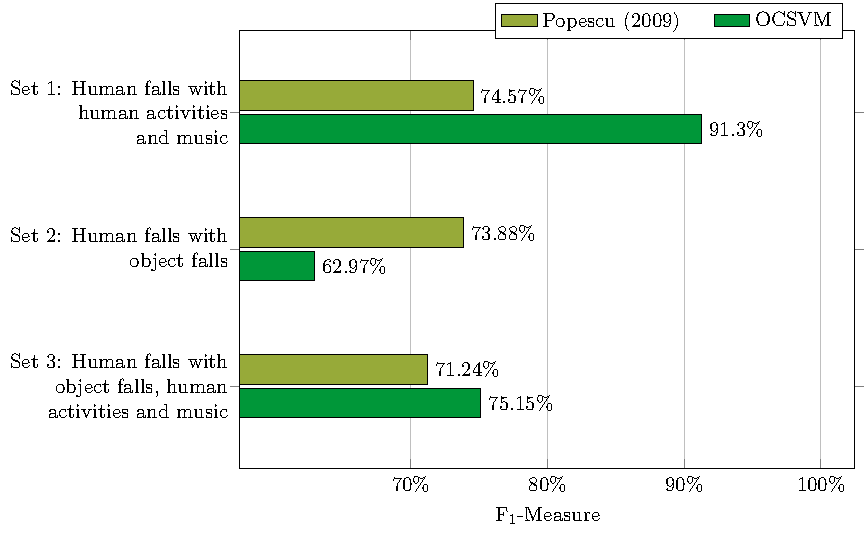
\includegraphics[width=\columnwidth]{img/cin_only_ocsv/res_noisy.pdf}
	\caption{Results in noisy conditions for the three test cases. ``Set 1'' comprises human falls, human activities and music. ``Set 2'' comprises human falls and object falls. ``Set 3'' comprises human falls, object falls, human activities, and music.} \label{fig:res_noisy}
\end{figure}




%\label{sec:ocsvm}}
\section[End-To-End Unsupervised Approach employing CNN-AE]{End-To-End Unsupervised Approach employing Convolutional Neural Network Autoencoders} 
\label{sec:autoencoder}



In recent years, thanks to the success of deep learning methods have become increasingly popular the feature learning approaches that independently transform the raw data inputs to a representation that can be exploited in machine learning tasks, minimizing the need of prior knowledge of application domain. 
Furthermore, such approaches are often able to generalize well real-world data compared to traditional hand-crafted features \cite{Principi14c}, resulting in an increase in performance of classification or regression tasks. The end-to-end learning is a particular example of feature learning, where the entire stack, connecting the input to the desired output, is learned from data \cite{muller2006off}. As in feature learning, only the tuning of the model hyperparameters requires some expertise, but even that process can be automated \cite{bergstra2013making}.

In this section, an end-to-end acoustic fall detection approach is presented. A deep convolutional neural network autoencoder is trained with the signals, gathered by the Floor Acoustic Sensor (\secref{sec:sensor}), corresponding to sounds that commonly occurring in a home (e.g., voices, footsteps, music, etc.). Since the sound produced by a human fall should be considerably different from the ones used for the training, it will be recognized as ``novelty'' by the network and classify as Fall. 
The performance of the algorithm has been evaluated on a subset of the dataset described in \secref{sec:dataset}, which contains human fall events simulated by employing the “Rescue Randy” human mimicking doll \cite{Werner2011,zigel2009method,alwan2006smart} and sounds related to common human activities.
Dieleman \textit{et al.} \cite{dieleman2014end} address the content-based music information retrieval tasks, investigating whether it is possible to apply end-to-end feature learning directly to raw audio signals instead that on a spectrogram representation of data.   
Up to the authors' knowledge, the end-to-end strategy has never been applied to a unsupervised fall detection approach with acoustic sensors. However, many works in other research fields can be founds in literature. 
Their convolutional neural networks trained on raw audio signals do not outperform a spectrogram-based approach in the automatic tagging task but are able to autonomously discover frequency decompositions from raw audio, as well as phase and translation-invariant feature representations.
The contribution is a novel fall detection method which exploits the end-to-end approach, resulting in a reduction of the engineering effort needed to design the system, with respect to those method that used features extracted from input signals. Is also shown that it can achieve good performance, higher than two state-of-the-art systems chosen for a comparison.


\subsection{Proposed System}
\label{sec:proposedApproach}

\begin{figure}[htb]
	\centering
	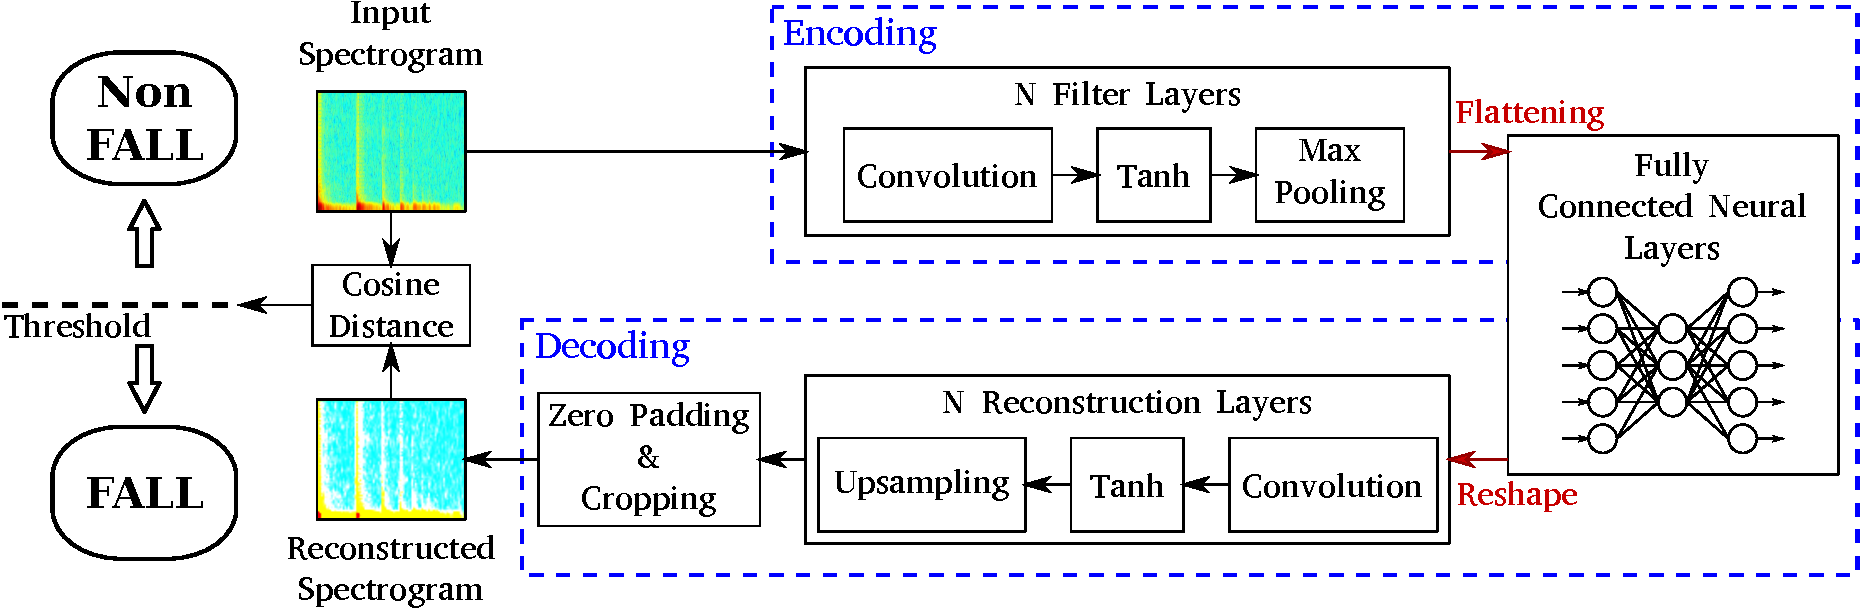
\includegraphics[width=\columnwidth]{img/wirn2017/approccioComplessivo.pdf}
	\caption{The proposed approach scheme.}\label{fig:overall}
\end{figure}

In the state of the art the majority of fall detection systems are logically designed as a cascade of elements which perform some sub-task (e.g. feature extraction, modeling, classification, ecc.).
%The minimal toolchain is composed by the feature extraction, modeling and classification blocks.
Each task is independently developed and generally requires the tuning of a number of hyperparameters using an experimental procedure and some a prior knowledge about the domain of the problem. 

The proposed approach, showed in \figref{fig:overall}, is designed according to the end-to-end paradigm and then, the entire stack, connecting the input to the desired output, is learned from data. 
End-to-End is a feature learning strategy that, in presence of sufficient training data, may result in better performance than systems based on handcrafted features, since the training procedure automatically select the salient information.
Therefore, if were possible to analyze the feature learned by the network with end-2-end strategy, there should be clues about what
kind of information is important for a specific task.

The system core is a deep convolutional neural network autoencoder. Some exhaustive discussion about this type of network can be easily  found in literature \cite{ng2011sparse,krizhevsky2012imagenet,marchi2017deep}. 
The network input consists of the normalized log-power spectrograms of the signals calculated with a STFT on windows of 32 ms and overlapped by 50\%.
Due to the presence of fully-connect neural layers, the input dimensions must be fixed. After having identified the widest spectrogram extracted from the dataset, the other ones have been extended with some AWGN frames added at the end. Each input consist in a $f\times t$ matrix, where $f$ are the positive points of discrete Fourier transform and $t$ are the number of windows considered in time.
The output of the autoencoder are the reconstructed spectrograms. To classify an event, a distance measurement between input and output must be made with some heuristic. If the distance exceeds a certain threshold, automatically defined by the algorithm during the training phase, the system label the output as "Fall" or as "Non Fall" otherwise. In this work the cosine distance has been used:

%f=129 t=197

\begin{equation}
D_C(v,u)=1-\frac{u\cdot v}{\left\|u \right\|\left\|v \right\| }= 1- \frac{\sum_{k=1}^{n}u(k)v(k)}{\sqrt{\sum_{k=1}^{n}u(k)^2}\sqrt{\sum_{k=1}^{n}v(k)^2}}
\end{equation}
where $u$ and $v$ are the the vectors obtained flattening the input and the output spectrograms and $n$ are the length of this vectors. 
According to the cosine definition, the value of the distance always has a value between $-1$ and $+1$, where $+1$ indicates two equal vectors while $-1$ indicates two opposite vectors.
The added AWGN part of the spectrums was not considered to calculate the distance. The choice of this heuristic allowed to make distance measurements independents of the size of the initial spectrum.
The structure of the autoencoder is not defined a priori, but it is chosen through a phase of cross-validation during which the network parameters are varied with a random search strategy.

\subsection{Experiments}
\label{sec:endtoend_experiments}
In this section are described the composition of the dataset used in this work and the experimental set-up.

\subsubsection{Data Used} 

The instances used in this approach are summarized in table \tableref{tab:endtoend_dataset}.
It is composed of two type of sounds: the first, namely novelty, comprises several human fall sounds that have been simulated by means of a human-mimicking doll employed in water rescues. The doll has been dropped from upright position and from a chair, both forward and backward. The drops have been then repeated at three distances from the FAS, i.e., 2, 4 and 6 m, for a total of 44 events, all included in the “Human fall” class. The second type, i.e, the background, comprises sounds of normal activities (voices, footsteps, etc.) for a total of 1218 s, and three musical tracks\footnote{W. A. Mozart, ``Piano trio in C major''}\footnote{Led Zeppelin, ``Dazed and confused''}\footnote{Led Zeppelin, ``When the levee breaks''}, for a total of 1498 s, played from a loudspeaker and acquired back with the FAS.
In addition, the signals of the second type have been employed alone and to create noisy versions of human falls occurrences in order to assess the algorithm in presence of interferences.
The signals have been acquired with a sampling rate equal to 44.1 kHz and 32 bit depth. Based on previous experience in using the FAS, in order to exploit the acoustic characteristics of the sensor, signals have been downsampled to 8 kHz and the resolution has been reduced to 16 bit.


\begin{table}[t]
	\caption{Composition  of the dataset.}
	\label{tab:endtoend_dataset}
	\begin{center}
		\begin{tabular}[t]{c>{\centering}m{5cm}c}
			
			\hline
			\textbf{Class} & \textbf{Nr. of occurrences} & \textbf{Total length (s)} \\ %\cline{2-5} 
			%& \hspace{8pt}Clean\hspace{8pt}  & \hspace{6pt}Clean\hspace{6pt}   \\ 
			\hline

			$\,$ Human Falls $\,$ 	& 44    &   76     \\
			Human Activity  		& 665   &   1218     \\
			Music					& 776   &	1498	\\
			%				 Classic Music       	& 441   &   882     \\
			%				 Rock Music       		& 335   &   616     \\
			\hline
		\end{tabular}
	\end{center}
\end{table}

\subsubsection{Experimental Setup}

Since in this work a novelty approach is presented, the dataset has been divided in two groups: the former composed only of background sounds (i.e human activity sounds and musical background) used for the training; the latter composed of both background sound and novelty sounds, i.e, the human falls, used in development and test phase.
In order to assess the classification accuracy in noisy conditions, a second version of human fall sounds were crated in which a musical background was recorded and then digitally added to the fall events.

The input spectrograms of the audio signals has been calculated with a fft point number of 256 and a windows size of 256 samples (32 ms at sample rate of 8000 kHz). The longest spectrogram present in the dataset is composed of 197 frame. Therefore the resulting input matrix  dimension $f\times t$ is $129\times 197$.
The optimization of the experiment hyper-parameters has been carried out using the random-search technique. \tableref{tbl:hyper-params} shows the parameters used in the random-search, and their ranges. The parameters of the network architecture are related only to the encoding part of autoencoder since the decoding part is its mirrored version. 
Instead other parameters, described below, have been set to the same value for all experiments. The activation function for each layer, whether they are convolutional or fully connected, have been set to $tanh$. ``Adam'' \cite{kingma2014adam} has been used as optimization algorithm for the traing phase. The loss function used was $mlse$. The initialization algorithm for the weight of the autoencoder was Glorot Uniform \cite{glorot2010understanding}. The number of epoch has been set to 1000, while the patience, that is the number of epoch without an Auc improvement on a devset to wait before stopping the training phase, has been set to 40.

In order to implements a 4 fold cross-validation, the signals not being part of training-set have been divided in four folds, each composed of 11 human falls and 11 non-falls signals. Then, one fold has been used as validation-set and the remaining three for calculating the performance in test phase. In cross-validation phase the scores have been evaluated in term of AUC. Here also the optimal thresholds have been infer by searching points on ROC curves closest to the $(0, 1)$: $ d_{min} = \sqrt{(1-fpr)^{2}+(1-tpr)^{2}} $.
At the end the final performance has been evaluated in term of  $ F_1 -Measure$ by mediating the results obtained on individual folds.

\begin{table}[t]
	\caption{Hyper-parameters optimized in the random-search phase, and their range.}\label{tbl:hyper-params}
	\centering
	\footnotesize
	\resizebox{\textwidth}{!}{
	\begin{tabular} {|c | c | c|| c | c | c|}
		\hline
		Parameter 		& Range & Distribution &Parameter & Range & Distribution\\  
		\hline\hline
		Cnn layer Nr. 	& [1-3]& uniform & Batch size	&	[10\%-25\%] & log-uniform\\
		\hline
		Kernel shape 	& [3x3-8x8]& uniform & Max pool shape & [1x1-5x5] & uniform \\
		\hline									
		Kernel Nr. 		& [4-64]& log-uniform & Max Pool & All\tablefootnote{After each Conv. layer}-Only end\tablefootnote{At the end of cnn part}& uniform \\
		\hline                                     
		MLP layers Nr. 	&	[1-3]& uniform & Dropout & [Yes-No] & uniform\\% dense-layer da uno a tre perchè quello interno ci sta sempre + da 0 a 2 di quelli messi dopo 
		\hline
		MLP layers dim.	&	[128-4096]& log-unifom & Drop rate	&	[0.5-0.6] & normal\\
		\hline
		Stride & [1x1-3x3]& uniform & Learning rate	&	[$10^{-4}$-$10^{-2}$]  & log-unifom\\
		\hline
		
	\end{tabular}}
\end{table}
Since this approach share the same train-set (\tableref{tab:trainComposition}) and test-set (\secref{tab:set1Composition}) that has been used in \secref{sec:ocsvm_approach} for both the clean and noisy conditions, the results scored here were compared with those obtained showed in \figref{fig:res_clean} and related to Set 1.

\begin{table}[t]
	\caption{Best hyper-parameters find in random-search phase for \textit{clean} and \textit{noisy} condition}\label{tbl:best-clean-params}
	\centering
	\footnotesize
	\resizebox{\textwidth}{!}{	\begin{tabular} {|c |  c | c | c | c ||  c | c | c | c |}
			\hline
			&\multicolumn{4}{|c||}{Clean}&\multicolumn{4}{c|}{Noisy}\\
			\hline
			Parameter	                        & Fold1             &Fold2          &Fold3      & Fold4     & Fold1         & Fold2         & Fold3         & Fold4\\
			\hline
			Cnn layer Nr.                       & 3                 & 3             & 3         & 2         & 3             & 3             & 3             & 3\\
			\hline
			Kernel shape                        & 8x8               & 7x7           & 5x5       & 8x8       & 8x8           & 7x7           & 8x8           & 8x8 \\
			\hline
			Kernel Nr. 	                        & [16,16,8]         & [32,16,16]    & [8,8,8]   & [32,16]   & [32,32,8]     &  [32,32,8]    &  [32,32,32]   & [8,8,8]\\
			\hline
			Max Pool Position	                &only end           &only end       & all       & all       & only end      & only end      & all           & only end\\
			\hline
			Max pool shape	                    & 5x5               & 3x3           & 5x5       & 4x4       & 3x3           & 5x5           & 5x5           & 3x3\\
			\hline
			Stride	                            & 3x3               & 3x3           & 1x1       & 3x3       & 3x3           & 3x3           & 1x1           & 3x3\\
			\hline
			MLP layers Nr.                      & 2                 & 1             & 1         & 1         & 2             & 2             & 1             & 3\\
			\hline
			MLP layers dim.	                    & [16,231]          & 96            & 32        & 32        & [48,153]      & [16,2084]     & 128           & [48,1952,1952]\\
			\hline
			Learning rate $(\times\num{e-4})$   &4.89               &  4.08         & 15.09     &  15.44    & 1.56          &  4.46         & 1.01          &  1.00\\
			\hline
			Batch size		                    & 11.26\%           & 10.81\%       & 13.59\%   & 21.10\%   & 20.06\%       & 12.55\%       & 13.51\%       & 13.13\%  \\
			\hline
			Drop rate		                    &0.64               &0.57           & 0.53      & 0.55      & 0.58          &0.53           & 0.55          & 0.59\\
			\hline
			
	\end{tabular}}
\end{table}

\subsection{Results}
The results for both clean and noisy are reported in \figref{fig:endtoend_results}. The comparative algorithms are denoted with ``Popescu (2009)'' and ``OCSVM'' respectively, while the proposed approach is named ``Autoencoder''. It is immediately clear that the proposed approach outperforms the other in both conditions. In fact, in clean condition, it gains about 1\% compared to ``OCSVM'' and about 18.6\% compared to ``Popescu (2009)''. Moreover the proposed algorithm results to be very robust in noisy condition, %where the score of ``OCSVM'' falls down %by 30.65\% while the score of  ``Popescu (2009)'' remains around the previous case.
whereas both other cases get worse a bit.
In particular the performance improves by 3.72\% with respect to ``OCSVM'' and by 20.45\% with respect to ``Popescu (2009)''. Clearly the end-to-end method seems insensitive with respect to the corrupted human fall signals when the novelty sounds are dissimilar respect to normality model learned from the background sounds. 
In \tableref{tbl:best-clean-params} are reported the hyperparameters that have led to the results discussed above.

Furthermore other experiments were made up with a manual tuning of parameters. Particularly have been investigated deeper architectures composed up to 5 convolutional layer. We found that increasing the depth on cnn part (5 layers) with a different kernel number for each layers of [32,32,16,16,8] and a kernel dimension for all layers of 4x4, a max pooling after only the first three convolutional layer of 2x2 and two MLP layer of 1024 and 512, leads to considerable improvements. In effect the final $ F_1 -Measure$ rise up to 95,42\%  in both clean and noisy condition. 
%\textcolor{red}{per motivare che noisy is better than clean direi che è dovuto allla variabilità degli esperimenti (inizializzazioni varie ecc..) visto che cmq c'è lo scarto di un solo mezzo punto. Se ripetessimo gli esperimenti potremmo ottenere risultati leggermente diversi ( considerando anche che siamo anche in cross-validation) }


\begin{figure}[htb]
	\centering
	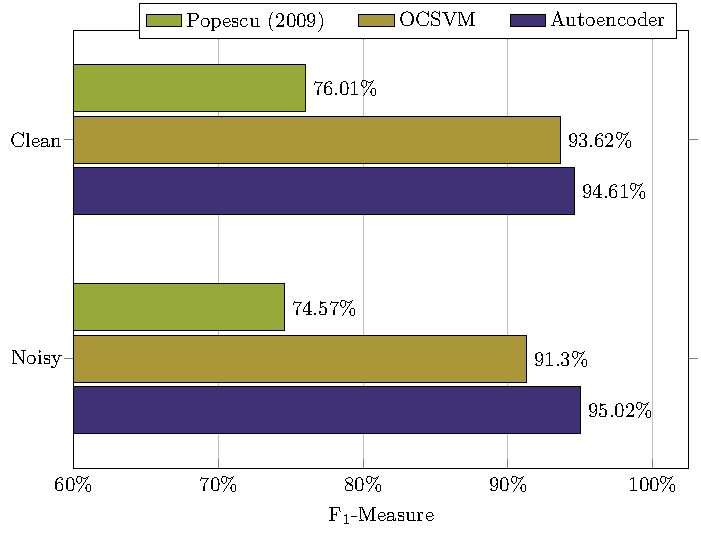
\includegraphics[width=0.75\columnwidth]{img/wirn2017/grafTex/results.pdf}
	\caption{Results in \textit{clean} and \textit{noisy} conditions for the three test cases.} 
	\label{fig:endtoend_results}
\end{figure}

\subsection{Remarks}
The methods presented is an end-to-end approach composed by a deep-convolutional-autoencoder with a downstream threshold classifier, that is a purely unsupervised approach to acoustic fall detection.
Our method exploits the reconstruction error of the autoencoder. When a sound that the network has never seen in training phase occurs, the reconstruction error raise up allowing the recognition of novelty.
The algorithm has been trained with a large corpus of background signals, i.e, human activity noise and music, and evaluated with human-fall sound and other instances of background sounds. It has been evaluated in two different condition: the first with a clean version of human fall sounds and the second with corrupted version of the same.
The results showed that the proposed solution leads to an average improvement about 20\%  with respect to the \cite{Popescu2009} and about 2.3\% towards the OCSVM based approach.

% this approach will be assessed in a more realistic scenario including, in the test phase, others sound topologies such as falls of different objects, street sounds, etc., that could compromise the classification. In fact those sounds are much more similar to the human falls and could lead to a worse performance. In addition, having regard the results obtained with a manual tuning of parameters, deeper network architectures in combination with Recurrent Neural Network will be thoroughly investigated.



\graphicspath{{6_Semi-Unsupervised_approaches/}}
\chapter{Semi-Unsupervised Approach}

Unsupervised methods, consider a human fall as an event that deviate from normality and they are based on one-class classifiers. The main advantage of an unsupervised methods for fall detection is that it can works without knowing any examples related the the class of interest, i.e. the human fall. As aforementioned, this should be the perfect way to go in an application like this, where what we are interested in is very difficult to retrieve or we only have very few data available, but the principal weakness of an unsupervised system is that certain events deviate from normality as the human fall (e.g., the fall of an object), thus they may produce false alarms.
In this Chapter, two types of methods are described: in \secref{sec:user_aided_cin} a OCSVM used-ided method is exposed, while \secref{sec:siamese_few_shot} present an approach based on Siamese neural network for one-shot learning, both of them assessed with samples related to R0 room of the employed dataset \secref{sec:dataset}. An extension of the Siamese approach is presented in \secref{sec:siamese_few_shot} where the entire dataset presented in \secref{sec:dataset} has been used.




\section{A Combined One-Class SVM and Template Matching Approach for User-Aided Human Fall Detection}
\label{sec:user_aided_cin}

The approach proposed here, is the extension of the one presented in \secref{sec:ocsvm_approach} thus, consists of a combined One-Class Support Vector Machine (OCSVM) based method and template-matching classifier that operate in cascade. The template-matching classifier operates in a user-aided supervised manner and it is employed to reduce such errors by using a set of templates that represent these events. Templates are identified by the user that marks the occurrence of a false positive instead of a true human fall event. 
As shown in the previous section, ``unsupervised methods'' are able to overcome the need of manual tuning of ``analytical methods'' and the necessity of a large labelled dataset of ``supervised methods''. In ``unsupervised methods'', falls are discriminated from non-falls based on a model of ``normality'' constructed from a large amount of non-fall events. However, certain events differ from the ``normality'' as human falls, and they may induce the classifier to produce false alarms. As an example, \figref{fig:time_ha} and \figref{fig:spec_ha} show respectively the waveform and the spectrogram of a segment of ``normal'' human activity (footsteps and speech) \figref{fig:time_hf} and \figref{fig:spec_hf} show the waveform and the spectrogram of a segment of human fall, and \figref{fig:time_bf} and \figref{fig:spec_bf} the waveform and the spectrogram of a book fall. The figures show clearly that both falls signals differ significantly from the human activity one, thus a classifier may be induced to consider the fall of a book as the fall of a person.

\begin{figure}[htbp!]
	\centering
	\begin{subfigure}[t]{0.5\columnwidth}
		\centering
		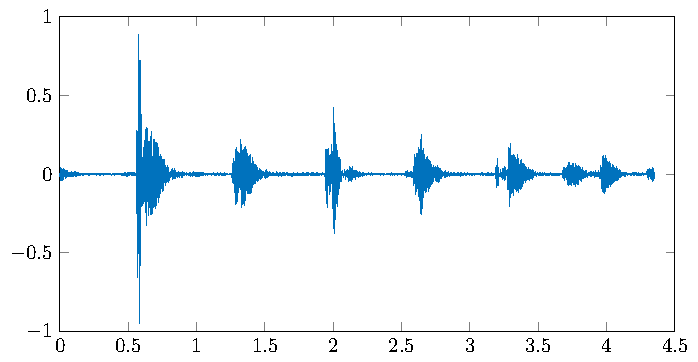
\includegraphics[width=0.9\textwidth]{img/cin/ha_time_.pdf}
		\caption{Normal human activity signal in the time domain.}\label{fig:time_ha}
	\end{subfigure}%
	\begin{subfigure}[t]{0.5\columnwidth}
		\centering
		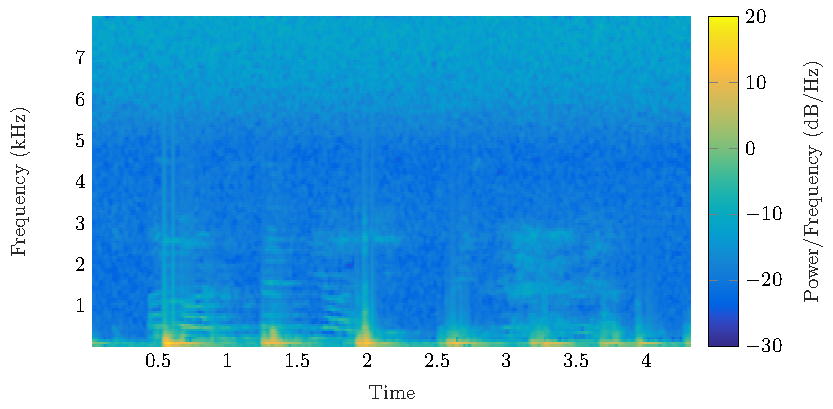
\includegraphics[width=\textwidth]{img/cin/ha_freq_.pdf}
		\caption{Normal human activity signal in the frequency domain.}\label{fig:spec_ha}
	\end{subfigure}
	
	\begin{subfigure}[t]{0.5\columnwidth}
		\centering
		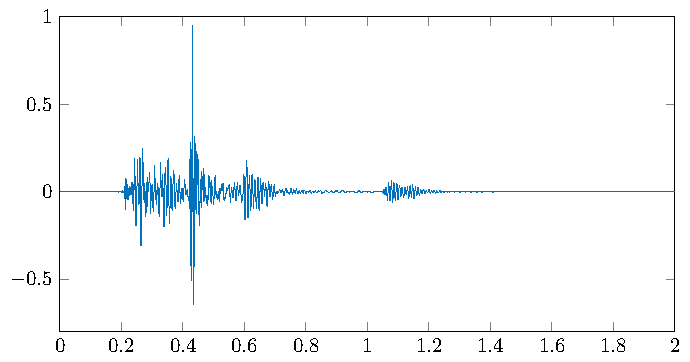
\includegraphics[width=0.9\textwidth]{img/cin/rndy_time_.pdf}
		\caption{Human fall signal in the time domain.}\label{fig:time_hf}
	\end{subfigure}%
	\begin{subfigure}[t]{0.5\columnwidth}
		\centering
		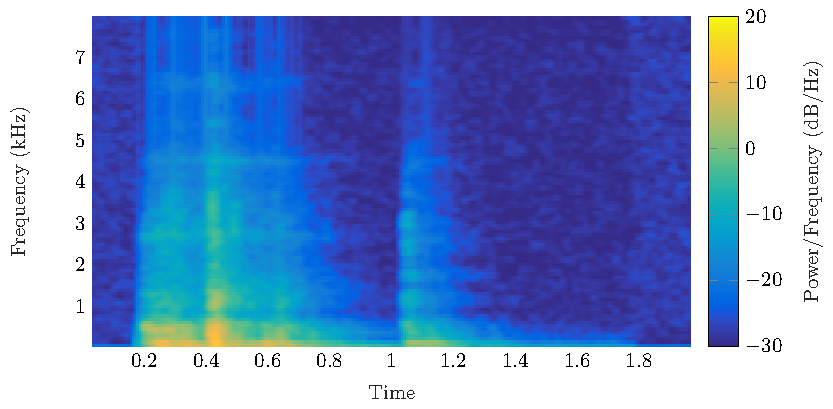
\includegraphics[width=\textwidth]{img/cin/rndy_freq_.pdf}
		\caption{Human fall signal in the frequency domain.}\label{fig:spec_hf}
	\end{subfigure}
	
	\begin{subfigure}[t]{0.5\columnwidth}
		\centering
		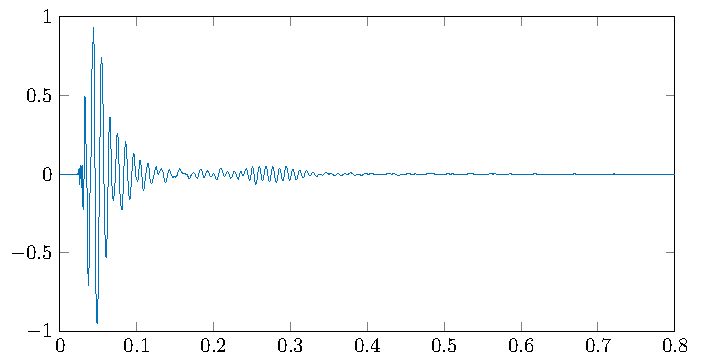
\includegraphics[width=0.9\textwidth]{img/cin/book_time_.pdf}
		\caption{Book fall signal in the time domain.}\label{fig:time_bf}
	\end{subfigure}%
	\begin{subfigure}[t]{0.5\columnwidth}
		\centering
		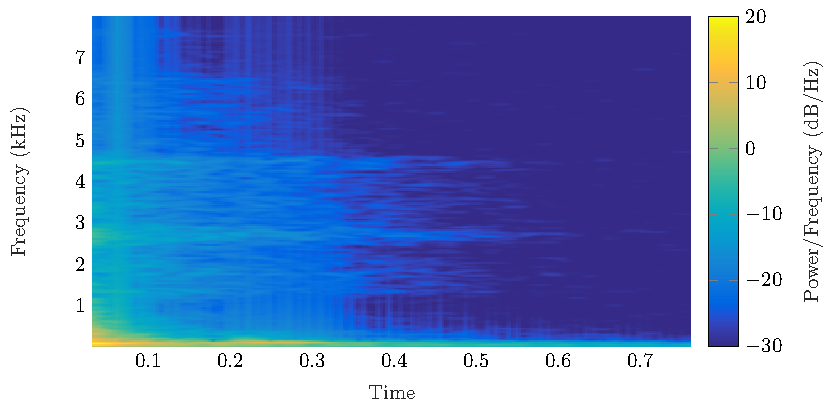
\includegraphics[width=\textwidth]{img/cin/book_freq_.pdf}
		\caption{Book fall signal in the frequency domain.}\label{fig:spec_bf}
	\end{subfigure}
	\caption{Time domain (on the left) and frequency domain (on the right) representation of a normal human activity signal (a-b), human fall signal (c-d), and book fall signal (e-f).}\label{fig:waveforms}
\end{figure}

The algorithm proposed in this paper reduces the problem by employing a multi-stage classification approach that combines a one-class classifier based on OCSVM with a template-matching stage. The OCSVM is trained unsupervisedly on a large corpus containing sounds that represent the ``normality''. On the contrary, the template-matching stage employs a set of templates represented by a small number of feature vectors marked as false alarm by the user. Thus, robustness against possible false alarms is achieved by using only few examples of false positive classes without the need of multiple sensors. An additional advantage with respect to the state of the art is that the proposed approach is able to evolve and improve after its initial training, since the template set can be augmented as non-falls events are detected.

\subsection{Proposed approach}
The proposed approach is composed of three stages \figref{fig:overall_ocsvm_user_aided}: the first (``Feature Extraction'') extracts MFCCs from the input audio signal and then GMSs to describe the entire audio segment. The second stage (``Abnormal Event Detection'') consists of a One-Class SVM classifier that discriminates between normal and abnormal sounds. Up to the authors' knowledge, OCSVM together with GMSs have never been jointly used for acoustic fall detection.  The third stage represents the innovative contribution of this paper for reducing false alarms in unsupervised approaches: it consists of a ``Template-Matching'' block that refines the output of the OCSVM and classifies the input data as fall or non-fall. The OCSVM is trained unsupervisedly on a large dataset of everyday sounds with the objective of discriminating normal from abnormal sounds. As aforementioned, the basic assumption is that the acoustic events related to human falls are ``rare'' respect to sounds normally occurring inside a home. The template-matching stage, on the other side, requires a set of ``template'' instances that represent rare events that can be confused with a fall. Referring to \figref{fig:overall_ocsvm_user_aided}, the ``Template-Matching'' stage is composed of a set of ``Templates'', a block that calculates the distance between the input GMS and the templates (``Euclidean Distance Calculation''), and a ``Decision'' block the decides whether the event is a fall or a non-fall by evaluating the magnitude of the distance.  The rationale here is that certain acoustic events are as abnormal as falls and confuse the OCSVM: the template-matching stage reduces false positives by using a set of examples related to the most confusing classes. In this work, the algorithm is ``user-aided'', i.e., templates are indicated by the user each time the OCSVM produces a false positive. This is shown in \figref{fig:overall_ocsvm_user_aided} with the person silhouette near the block that decides whether a detected fall is a false positive or not (``False Positive?''). In general, however, it is possible to create the templates set a-priori by recording several instances of possible false alarms events. Although rare, false alarm events (e.g., falls of objects) are certainly easier to reproduce in laboratory respect to human falls.

\subsubsection{Template Matching}
The template-matching classifier operates on a set of templates, i.e., supervectors, that can be defined a-priori or selected by the user when the OCSVM detects an abnormal sound that is not a human fall. Denoting with $\mathbf{x}$ the supervector of the input signal and with $\mathcal{Y} = \{\mathbf{y}_1,\ldots,\mathbf{y}_N\}$ the set of templates, the algorithm operates by calculating the Euclidean distance $D^{(i)} = \| \mathbf{x} - \mathbf{y}_i \|$ between the supervector to be classified and all the templates in the set. Indicating with $D_{min} = \underset{i}{\min}\,\,D^{(i)}$, the supervector $\mathbf{x}$ is classified as a fall if $D_{min}>\beta$ and as non-fall otherwise. The threshold $\beta$ is a hyperparameter of the algorithm that can be determined on a validation set.

\begin{figure}[t]
	\centering
	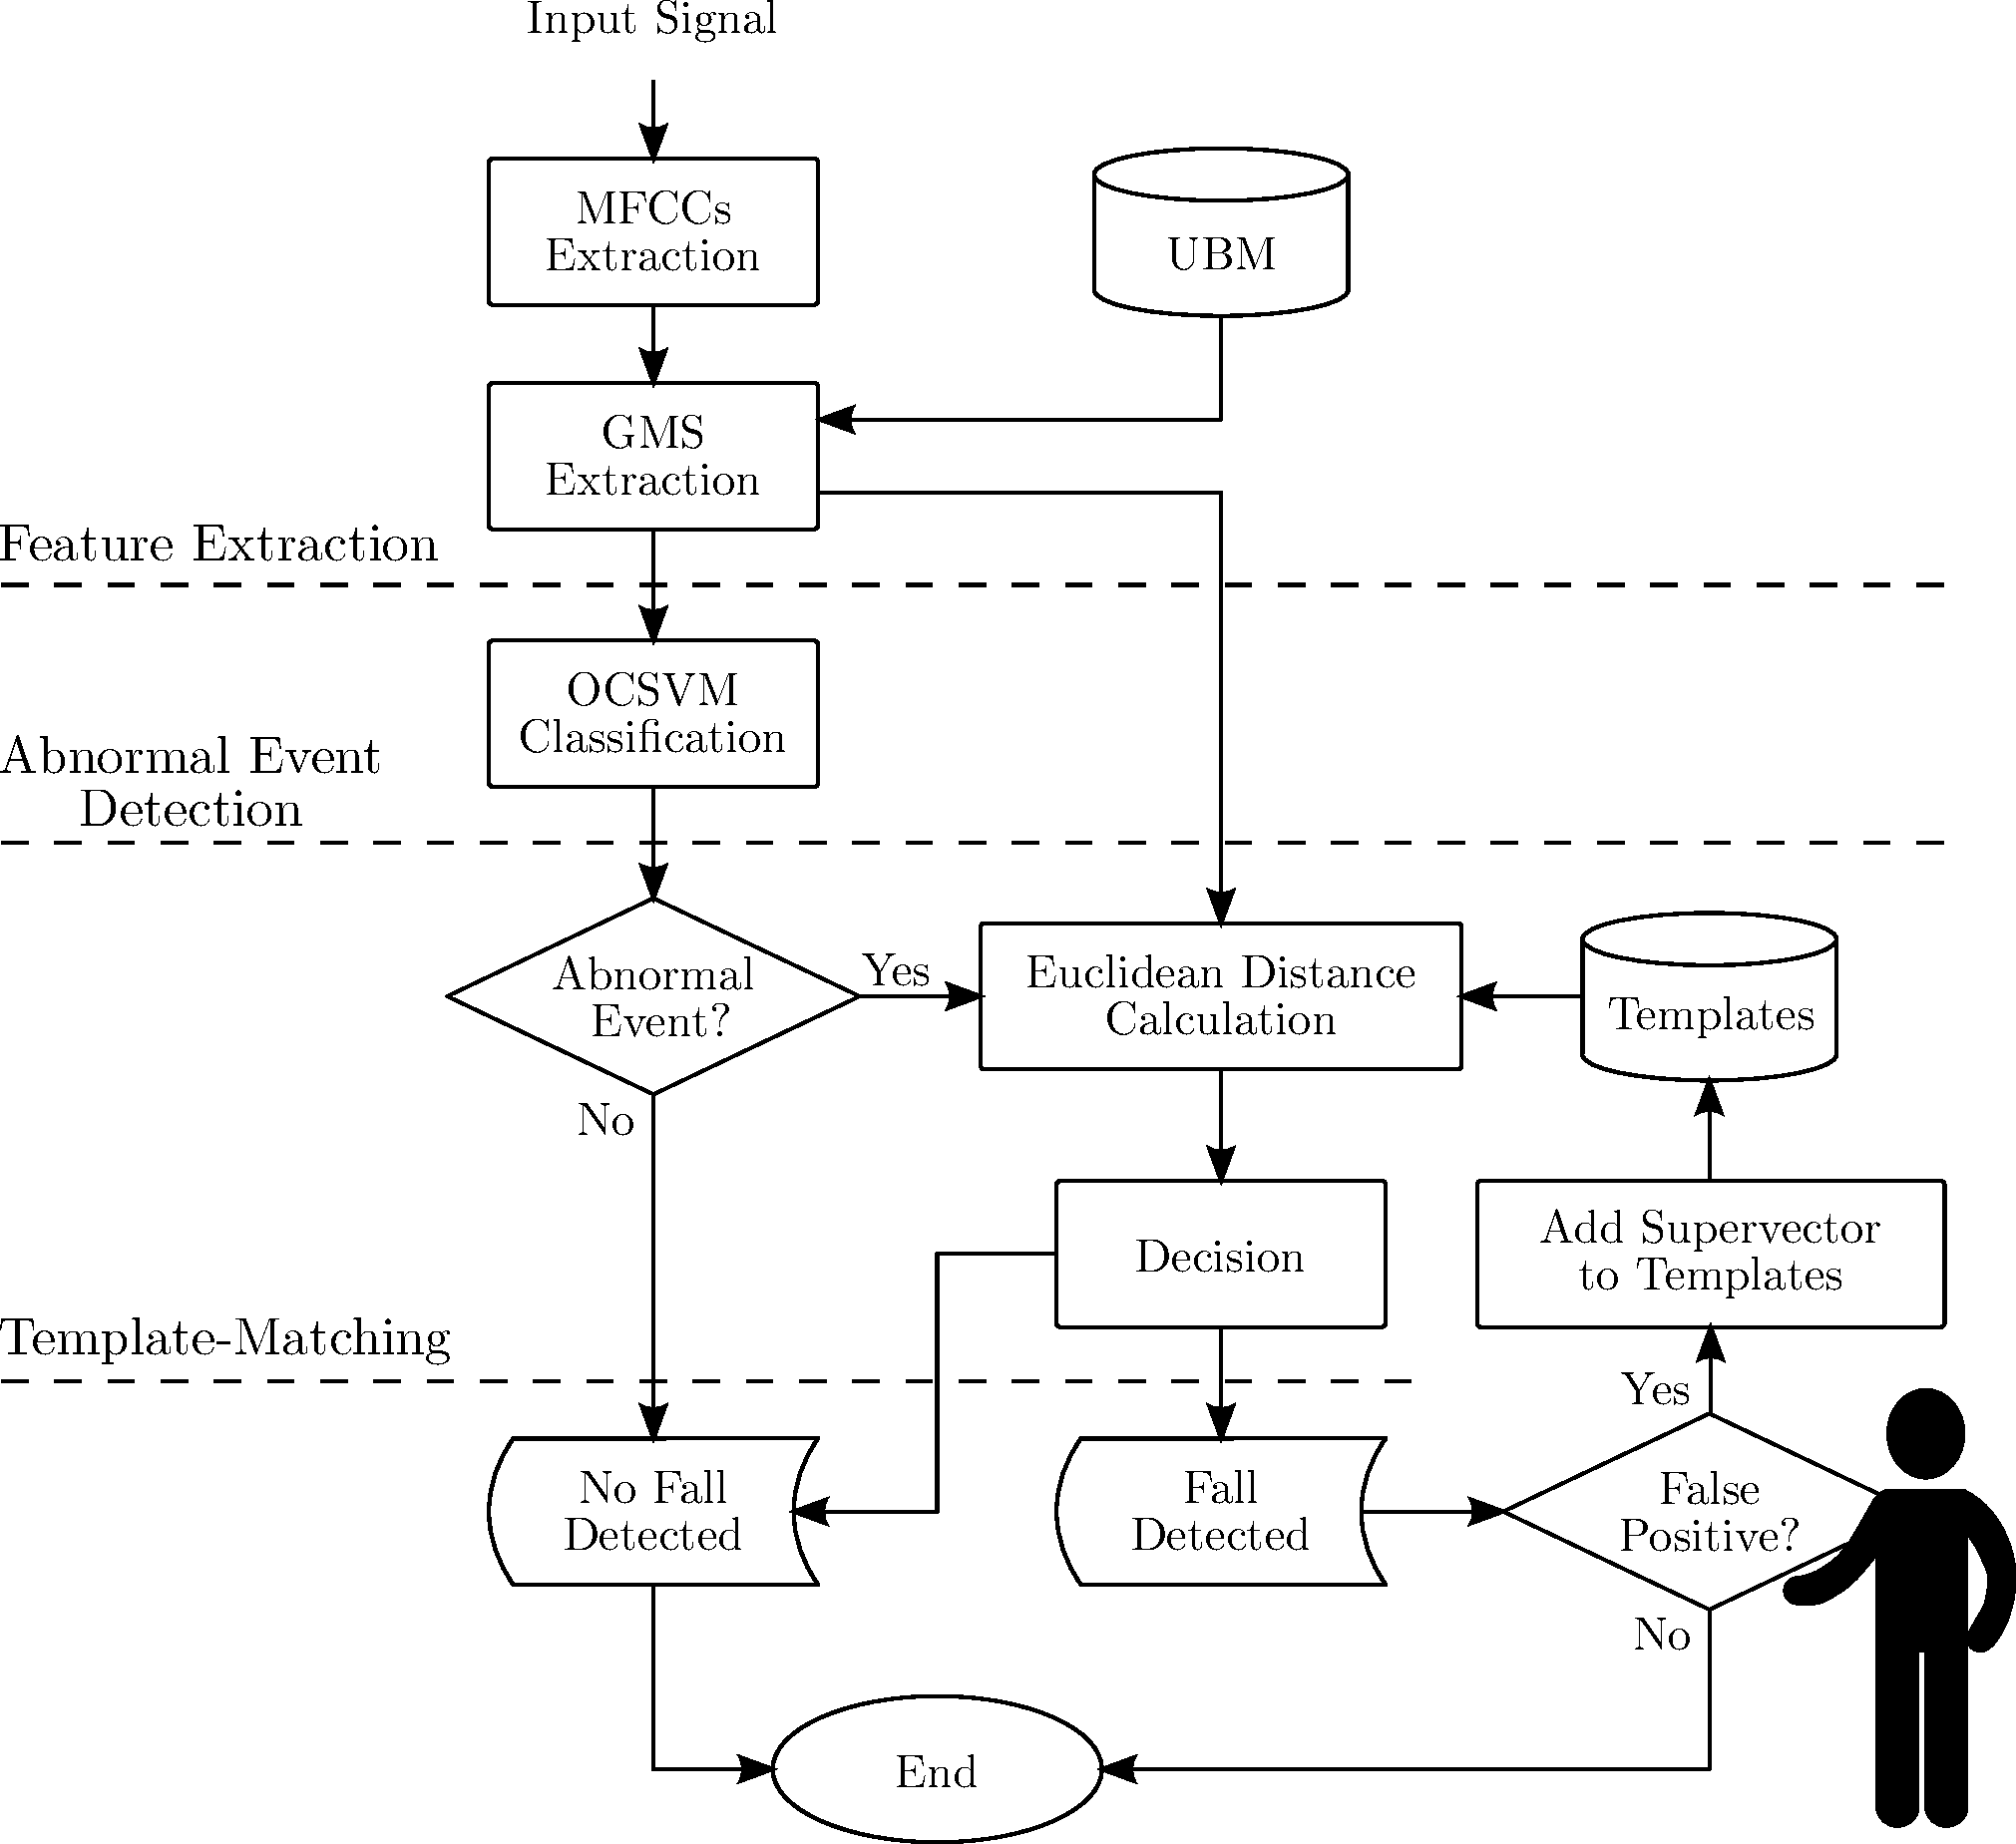
\includegraphics[width=0.95\columnwidth]{img/cin/approccioComplessivo.pdf}
	\caption{The block scheme of the proposed approach.}\label{fig:overall_ocsvm_user_aided}
\end{figure}

\subsection{Dataset}

The dataset employed in this method is the same used for the approach proposed in \secref{sec:ocsvm_approach} and reported in \tableref{tab:ocsvm_dataset}. Please refer to \secref{sec:dataset_cin_ocsvm_only} for the details.

\subsection{Experimental setup}
As in the system presented in \secref{sec:ocsvm_approach}, the dataset has been divided in one set for training the UBM and the OCSVM and three sets for evaluating the performance.
Training has been performed on the same set used for the OCSVM base algorithm presented in \secref{sec:ocsvm_approach} and shown in \tableref{tab:trainComposition}. The same three sets described in \secref{sec:experiment_ocsvm} has been used for the assessment and summarized below as a reminder:
\begin{itemize}
	\item Set 1: Human fall and background sounds (\tableref{tab:set1Composition_}).
	\item Set 2: Human fall and object fall sounds (\tableref{tab:set2Composition_}).
	\item Set 3: Human fall, object fall and background sounds (\tableref{tab:set3Composition_}).
\end{itemize}


\begin{table}[t]
	\centering
	\caption{Data used in ``Set 1''.}
	\begin{subtable}[t]{.6\textwidth}
		\centering		
		\caption{Composition  of ``Set 1''.}
		\label{tab:set1Composition_} % è lo stesso del capitolo 5. Lo riporto qui per comodità di lettura
		\begin{center}
			\begin{tabular}{K{3cm}K{3cm}}				
				\hline
				\textbf{Class} & \textbf{Nr.\ of occurrences} \\ 
				\hline
				$\,$ Human Falls $\,$ 	& 44    			\\
				Human Activity  		& 15		\\
				Music			  		& 29		\\
				%				 Classic Music       	& 15   		\\
				%				 Rock Music       		& 14  		\\		
				\hline
			\end{tabular}			
		\end{center}		
	\end{subtable}%
	\begin{subtable}[t]{.6\textwidth}
		\centering		
		\caption{Templates of ``Set 1''.}\label{tab:set1Template}
		\begin{center}
			\begin{tabular}{ccc}
				
				\hline
				\multirow{2}{1cm}{\textbf{Class}}	& \multicolumn{2}{c}{\textbf{Nr.\ of templates}}	\\ 
				\cline{2-3}
				&\textbf{Clean}&\textbf{Noisy}						\\
				%& \hspace{8pt}Clean\hspace{8pt}  & \hspace{6pt}Clean\hspace{6pt}   \\ 
				\hline
				Human Activity  		& 13	&	11 		\\
				Music       	& 8   	&	16		\\
				%				 Classic Music       	& 8   	&	16		\\
				%				 Rock Music       		& 0  	&	0		\\	
				\hline
				Total					& 21  	&	27		\\
				\hline
			\end{tabular}
			
		\end{center}
	\end{subtable}
	
	
\end{table}

\begin{table}[t]
	\centering
	\caption{Data used in ``Set 2''.}
	\begin{subtable}[t]{.6\textwidth}
		\centering
		
		\caption{Composition  of ``Set 2''.}
		\label{tab:set2Composition_}
		\begin{center}
			
			\begin{tabular}{K{3cm}K{3cm}}
				
				\hline
				\textbf{Class} & \textbf{Nr. of occurrences} \\ 
				%& \hspace{8pt}Clean\hspace{8pt}  & \hspace{6pt}Clean\hspace{6pt}   \\ 
				\hline
				$\,$ Human Falls $\,$ 	& 44    		\\				
				Basket      			& 7           	 \\
				Fork        			& 7           	 \\
				Ball       			& 8           	 \\
				Book        			& 7          	  \\
				Bag         			& 8          	  \\
				Chair       			& 7    			\\
				
				\hline
			\end{tabular}
			
		\end{center}
		
	\end{subtable}%
	\begin{subtable}[t]{.6\textwidth}
		\centering
		
		\caption{Templates of ``Set 2''.}
		\label{tab:set2Template}
		\begin{center}
			\begin{tabular}{ccc}
				
				\hline
				\multirow{2}{1cm}{\textbf{Class}}	& \multicolumn{2}{c}{\textbf{Nr.\ of templates}}	\\ 
				\cline{2-3}
				&\textbf{Clean}&\textbf{Noisy}						\\
				%& \hspace{8pt}Clean\hspace{8pt}  & \hspace{6pt}Clean\hspace{6pt}   \\ 
				\hline
				Basket  		& 55	&	57 		\\
				Fork       	& 39   	&	55		\\
				Ball      		& 11  	&	52		\\	
				Book  			& 26	&	57 		\\
				Bag       		& 26   	&	56		\\
				Chair       	& 86  	&	89		\\
				\hline	
				Total			& 243   &	366		\\	
				\hline
			\end{tabular}
			
		\end{center}
		
		
	\end{subtable}
	
	
\end{table}


\begin{table}[t]
	\centering
	\caption{Data used in ``Set 3''.}
	\begin{subtable}[t]{.6\textwidth}
		\centering
		
		\caption{Composition  of ``Set 3''.}
		\label{tab:set3Composition_}
		\begin{center}
			
			\begin{tabular}{K{3cm}K{3cm}}
				
				\hline
				\textbf{Class} & \textbf{Nr. of occurrences} \\ 
				%& \hspace{8pt}Clean\hspace{8pt}  & \hspace{6pt}Clean\hspace{6pt}   \\ 
				\hline
				$\,$ Human Falls $\,$ 	& 44    		\\				
				Basket      			& 3            	\\
				Fork        			& 4            	\\
				Ball       			& 4            	\\
				Book        			& 3            	\\
				Bag         			& 4            	\\
				Chair       			& 4    			\\
				Human Activity  		& 8   			\\
				Music			  		& 14   			\\
				%				 Classic Music       	& 7   			\\
				%				 Rock Music       		& 7   			\\
				
				\hline
			\end{tabular}
			
		\end{center}
		
	\end{subtable}%
	\begin{subtable}[t]{.6\textwidth}
		\centering
		
		\caption{Templates of ``Set 3''.}
		\label{tab:set3Template}
		\begin{center}
			\begin{tabular}{ccc}				
				\hline
				\multirow{2}{1cm}{\textbf{Class}}	& \multicolumn{2}{c}{\textbf{Nr.\ of templates}}	\\ 
				&\textbf{Clean}&\textbf{Noisy}						\\
				%& \hspace{8pt}Clean\hspace{8pt}  & \hspace{6pt}Clean\hspace{6pt}   \\ 
				\hline
				Basket      			& 52     &  57		\\
				Fork        			& 57     &  57 		\\
				Ball       			& 19     &  55  	\\
				Book        			& 53     &  57   	\\
				Bag         			& 50     &  56    	\\
				Chair       			& 89     &	89		\\
				Human Activity  	& 11   	 &	4		\\
				Music 			      	& 4   	 &	11		\\
				%							 Classic Music       	& 4   	 &	11		\\
				%							 Rock Music       		& 0   	 &	0		\\
				\hline	
				Total						& 335   &	386		\\	
				\hline
			\end{tabular}			
		\end{center}		
	\end{subtable}
	
	
\end{table}
The validation phase has been set following the same procedure described in section \secref{sec:experiment_ocsvm}: a cross-validation composed of four fold has been used for estimating the hyperparameter and  the final performance is calculated by using the cumulative true positives, false positives, and false negatives obtained by varying the test folds.
Differently from the previous method, the validation phase consisted not only in searching for the number of components of the UBM and the parameters ($\nu$ and $\gamma$) of the OCSVM, but also the value of the threshold $\beta$ in the template-matching stage. The values assumed by these variables are summarized in \tableref{tab:parameter}.
The method employed for the template-matching decision threshold is explained in \secref{ssec:templateThreshold}.

%\subsection{Comparative method}

\begin{table}[t]
	\centering
	\caption{Hyperparameters of the algorithm and search space explored in the validation phase. The search space of the template-matching threshold $\beta$ is not reported, since is determined with the procedure described in \secref{ssec:templateThreshold}. }
	\label{tab:parameter}
	\begin{tabular}{c |c | c}
		\hline
		\textbf{Stage} & \textbf{Hyperparameter} & \textbf{Range} \\
		\hline
		UBM & $J$ & $1, 2, 4, \ldots , 64$\\
		\hline
		\multirow{2}{*}{OCSVM} & $\nu$ & $0.1, 02, \ldots, 1.0$ \\
		&$\gamma$ & $2^{-15}, 2^{-13}, \ldots,2^{3} $ \\
		\hline
		Template-matching & $\beta$  & See \secref{ssec:templateThreshold}\\
		\hline
	\end{tabular}
\end{table}

All the aforementioned datasets require a set of templates for the template-matching stage of the algorithm. In the case of object falls, the set of templates has been created by classifying a set of 372 object falls with the OCSVM and selecting the occurrences misclassified as human falls. In the case of background sounds, the set of templates has been created by calculating the Euclidean distance between each occurrence of the development-set and each occurrence of a set of 470 background signals and then selecting the segment whose distance is minimum. Details on the templates sets are shown in \tableref{tab:set1Template}, \tableref{tab:set2Template}, and \tableref{tab:set3Template} respectively for ``Set 1'', ``Set 2'', and ``Set 3''.


The proposed approach has been compared with the method from which it derives (\secref{sec:ocsvm_approach}) and the algorithm presented in \cite{Popescu2009} based on OCSVM (please revert to \paragref{par:popescu_mod} for the details) 

The performance has been evaluated in terms of F$_1$-Measure \eqref{eq:f1} 

\subsection{Choice of the template-matching decision threshold}\label{ssec:templateThreshold}
A key point of the proposed approach is the decision threshold $\beta$ in the template-matching stage. Choosing a too low value would result in a low number of false negatives and a high number of false positives. On the contrary, a too high value would result in a high number of false negatives and a low number of false positives. The choice of $\beta$ has been performed by calculating the minimum Euclidean distance between each fall and non-fall event in the validation set and the set of templates. \figref{fig:distr_clean} and \figref{fig:distr_noisy} show respectively the probability distributions for the three sets in clean and noisy conditions. The decision threshold $\beta$ has been chosen at the intersection point between the distribution of fall and non-fall distances. This choice represents a compromise that balances false positives and false negatives.

Observing clean condition distributions, in ``Set 1'' the two density are considerably overlapped, while in ``Set 2'' the overlap is modest. It is expected that the possible improvement of the template-matching stage will be more consistent for ``Set 2'' respect to ``Set 1''. ``Set 3'' contains human activity and music occurrences as ``Set 1'' and object falls as ``Set 2'': indeed, the probability distributions (\figref{fig:distr_clean_set3}) are more distinct respect to the ones of ``Set 1'', but not so much as the ones of ``Set 2''.

Noisy condition distributions, shown in \figref{fig:distr_noisy}, are in general less distinct compared to clean condition ones. The effect of noisy is to flatten the distances of the fall and non-fall classes, thus resulting in a less discriminative capabilities of the classifier. Thus, it is expected that the performance improvement in noisy conditions will be more modest respect to the one obtained in clean condition.

\begin{figure}[t]
	\centering
	\begin{subfigure}{0.9\columnwidth}
		\centering
		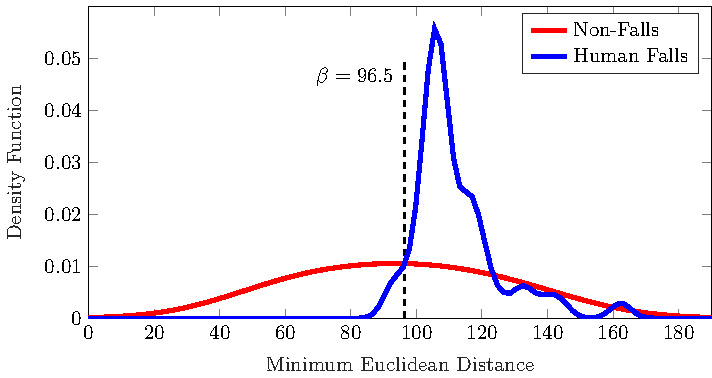
\includegraphics[width=0.98\columnwidth]{img/cin/distribuzione_Caso1_Clean.pdf}
		\subcaption{Probability distributions related to ``Set~1''.}\label{fig:distr_clean_set1}
	\end{subfigure}\hspace{1pt}
	\begin{subfigure}{0.9\columnwidth}
		\centering
		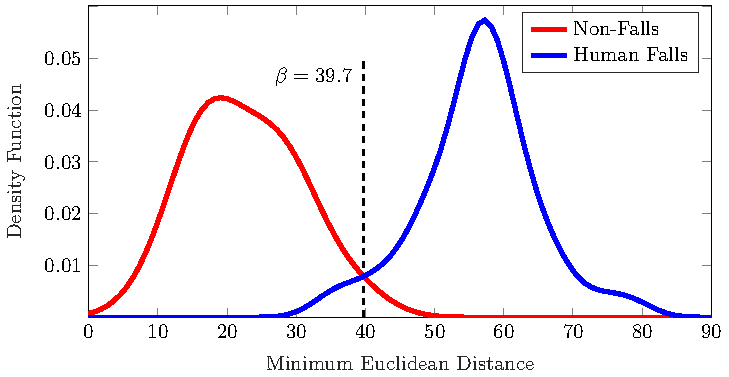
\includegraphics[width=\columnwidth]{img/cin/distribuzione_Caso2_Clean.pdf}
		\subcaption{Probability distributions related to ``Set~2''.}\label{fig:distr_clean_set2}
	\end{subfigure}\hspace{1pt}
	\begin{subfigure}{0.9\columnwidth}
		\centering
		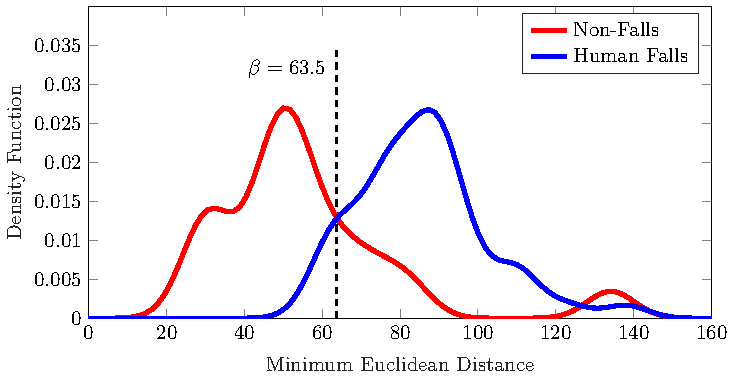
\includegraphics[width=\columnwidth]{img/cin/distribuzione_Caso3_Clean.pdf}
		\subcaption{Probability distributions related to ``Set~3''.}\label{fig:distr_clean_set3}
	\end{subfigure}
	\caption{Probability distributions of the minimum Euclidean distances among the template sets, and human falls and non-falls in \textit{clean} acoustic condition.}\label{fig:distr_clean}
\end{figure}

\begin{figure}[t]
	\centering
	\begin{subfigure}{0.9\columnwidth}
		\centering
		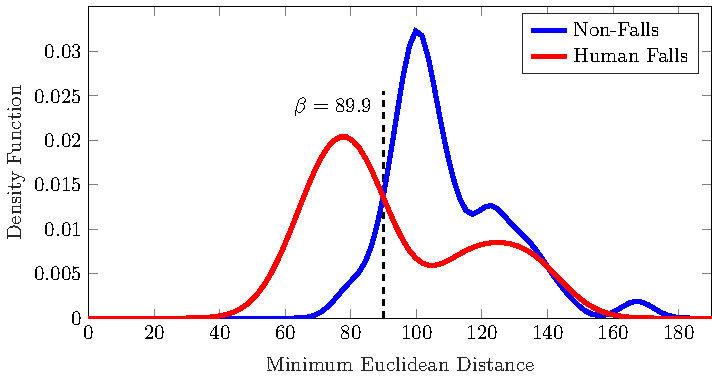
\includegraphics[width=0.98\columnwidth]{img/cin/distribuzione_Caso1_Noisy.pdf}
		\subcaption{Probability distributions related to ``Set~1''.}
	\end{subfigure}\hspace{1pt}
	\begin{subfigure}{0.9\columnwidth}
		\centering
		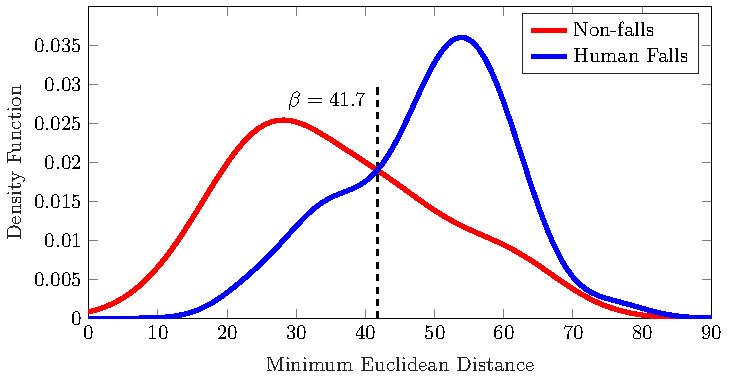
\includegraphics[width=\columnwidth]{img/cin/distribuzione_Caso2_Noisy.pdf}
		\subcaption{Probability distributions related to ``Set~2''.}
	\end{subfigure}\hspace{1pt}
	\begin{subfigure}{0.9\columnwidth}
		\centering
		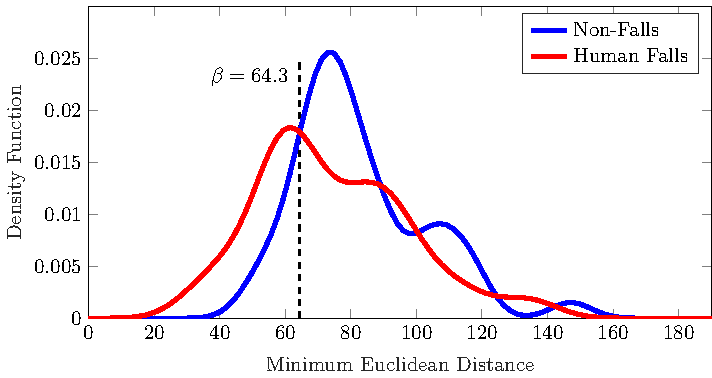
\includegraphics[width=\columnwidth]{img/cin/distribuzione_Caso3_Noisy.pdf}
		\subcaption{Probability distributions related to ``Set~3''.}
	\end{subfigure}%
	\caption{Probability distributions of the minimum Euclidean distances among the template sets, and human falls and non-falls in \textit{noisy} acoustic condition.}\label{fig:distr_noisy}
\end{figure}

\subsection{Results}
\figref{fig:res_clean_} shows the results in clean conditions obtained with and without the template-matching stage, respectively denoted as ``OCSVM+Template-Matching'' and ``OCSVM''. The results obtained with the method proposed in \cite{Popescu2009} are denoted with ``Popescu (2009)''. Observing the figure, it is evident that in all the three cases the template-matching approach is able to improve the performance with respect to ``Popescu (2009)'' \cite{Popescu2009} and the OCSVM only approach. In particular, in ``Set 1'', that comprises human falls, human activities and music, the performance improves by 2.03\% with respect to OCSVM and by 19.64\% with respect to ``Popescu (2009)''. This case can be considered as the least challenging of the three, since non-falls events are considerably different from falls ones. Conversely, ``Set 2'' comprises both human falls and object falls, thus it includes abnormal events whose pattern is similar to the one of human falls. The introduction of the template-matching stage considerably reduces the number of false positives, leading to an overall performance improvement of 20.76\%. ``Set 3'' comprises human falls, human activities, music and object falls and represents the most realistic test condition of the three. Introducing the template-matching stage, the performance improves by 7.64\%, leading to an F$_1$-Measure equal to 89.89\%. 

\begin{figure}[t]
	\centering
	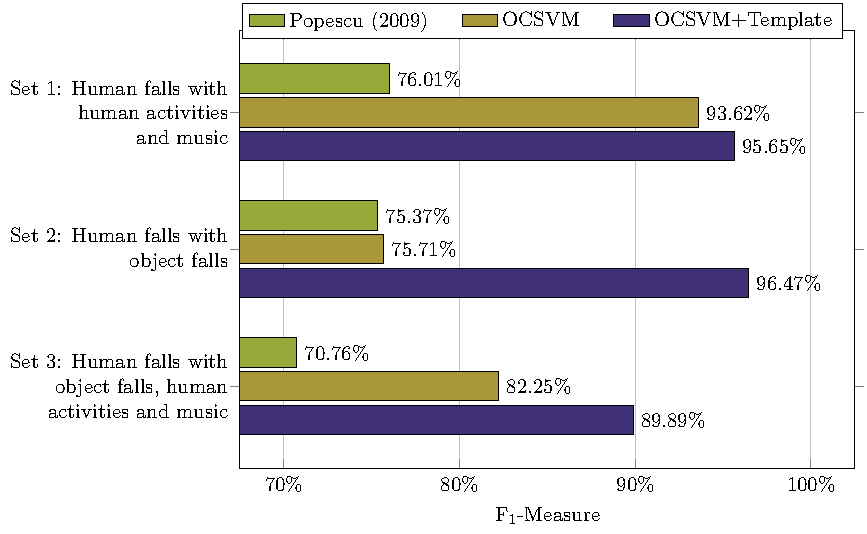
\includegraphics[width=\columnwidth]{img/cin/res_clean.pdf}
	\caption{Results in \textit{clean} conditions for the three test cases. ``Set 1'' comprises human falls, human activities and music. ``Set 2'' comprises human falls and object falls. ``Set 3'' comprises human falls, object falls, human activities, and music.} \label{fig:res_clean_}
\end{figure}

\figref{fig:res_noisy_} shows the results obtained for the three cases in noisy conditions. As expected, the performance decreases in all the three evaluated methods. In ``Set 1'', the performance decrease is modest (2.32\% for the OCSVM, 2.63\% for the proposed approach, and 1.44\% for ``Popescu (2009)''), demonstrating that the OCSVM is able to effectively reject non-fall events corrupted by music interference. The use of the template-matching stage increases the performance by 1.72\%, thus providing a significant improvement also in noisy conditions. In ``Set 2'', Template-matching provides a performance improvement of 8.02\% with respect to the OCSVM, leading to an F$_1$-Measure higher than 70\%. The improvement is lower with respect to the clean ``Set 2'', since the variability of the music interference makes the Euclidean distances of fall and non-fall classes more similar and is not sufficient to overcome the ``Popescu (2009)'' \cite{Popescu2009}. In ``Set 3'', the proposed approach improves the performance by 4.77\% with respect to OCSVM and by 8.68\% with respect to ``Popescu (2009)''.

In summary, the results demonstrated that the introduction of a template-matching stage significantly improves the performance both of the OCSVM only approach and of the method by Popescu and Mahnot \cite{Popescu2009}: averaging the results over ``Set 1'', ``Set 2'', and ``Set 3'', the absolute improvement with respect to the former is 10.14\% in clean conditions and 4.84\% in noisy conditions. With respect to the latter \cite{Popescu2009} the improvement is 19.96\% in clean conditions and 8.08\% in noisy conditions. As shown in \figref{fig:res_clean_} and \figref{fig:res_noisy_}, both in clean and noisy conditions the F$_1$-Measure of the method by Popescu and Mahnot \cite{Popescu2009} is close to 75\% in ``Set 1'' and ``Set 2'', and close to 71\% in ``Set 3''. The different behaviour compared to the OCSVM only approach can be attributed firstly to the different feature representation of the audio signal (MFCCs instead of supervectors). Secondly, to the strategy adopted for classification: in \cite{Popescu2009}, signals are divided in windows and a fall is detected if at least two consecutive windows are classified as fall. Differently, in the proposed algorithm, the overall signal is represented by a single supervector and classified as fall or non fall.

Comparing the results in clean (\figref{fig:res_clean_}) and noisy (\figref{fig:res_noisy_}) conditions, it is evident that techniques for reducing the impact of additive noise are needed. Additionally, the proposed solution requires the intervention of the user for selecting the templates after the first classification stage performed by the OCSVM. This aspect will be addressed in next sections in order to make the algorithm completely independent of the user, using a low number of examples related to human fall.

\begin{figure}[t]
	\centering
	\includegraphics[width=\columnwidth]{img/cin/res_noisy.pdf}
	\caption{Results in noisy conditions for the three test cases. ``Set 1'' comprises human falls, human activities and music. ``Set 2'' comprises human falls and object falls. ``Set 3'' comprises human falls, object falls, human activities, and music.} \label{fig:res_noisy_}
\end{figure}
\section{Few-shot Siamese Neural Networks employing Audio features
for Human-Fall Detection}
\label{sec:siamese_few_shot}
\section{Audio Metric Learning by using Siamese Autoencoders
for One-Shot Human Fall Detection}
\label{sec:siamese_one_shot}

\graphicspath{{7_other_contributions/}}
\chapter{Other contributions}\label{ch:other}

\section{An End-to-End Unsupervised Network for Timbre Transfer in Musical Applications}

A successful application of end-to-end computational intelligence in the field of image processing is the so-called ``style transfer'', i.e., the creative modification of a ``content'' image applying textures, strokes and colours from a  reference image providing stylistic information. In the audio field, however, and specifically with music signals, the task is yet to be properly defined and addressed.
More recently, researchers and machine learning developers asked themselves whether the algorithms that works for images were able to produce similar results with audio signals, and specifically, musical signals.
In the past years, several hybridization techniques have been proposed to synthesize novel audio content owing its properties from two audio sources. These algorithms, however, usually provide no feature learning, leaving the user, often intentionally, exploring parameters by trial-and-error. The introduction of machine learning algorithms in the music processing field calls for an investigation to seek for possible exploitation of their properties such as the ability to learn semantically meaningful features. The main aim of this work is to propose a method to tackle the so-called \emph{timbre transfer}, a topic that we consider being a sub-problem of the more general \emph{musical style transfer}. We adopt a Neural Network Autoencoder architecture and we enhance it to exploit temporal dependencies. In our experiments the architecture was able to modify the original timbre, resembling what it learned during the training phase, while preserving the pitch envelope from the input.


\subsection{Proposed approach}
\label{sec:architecture}

\subsubsection{Neural Network Architecture}
The proposed neural network architecture is designed to capture spectral characteristics of audio signals in the time and frequency domain. The architecture adopted to perform this task is an autoencoder, i.e., a neural network trained to copy its input to its output \cite{Goodfellow2016BookChap14}. A properly trained autoencoder, however, does not perform a simple copy operation, but learns significant characteristics of the training data. This property has been exploited in several different task in the literature, such as novelty detection \cite{Principi17a}, dimensionality reduction \cite{Hinton2006reducing}, and speech enhancement \cite{Lu2013speech}. Here, the capabilities of the autoencoder are used to transform the input data based on the characteristics of the training data. The rationale here is that the autoencoder will try to reconstruct the input based on the knowledge acquired during the training phase, thus transforming the input signal based on the characteristics of the training data. An overview of the proposed architecture is shown in Figure \ref{fig:modello} for the sake of clarity, and its details will now be presented.

\begin{figure}[t]
	\centering
	\includegraphics[width=\textwidth]{img/audioXsynth/architecture}

%	\def\svgwidth{\textwidth}
%	\input{7_other_contributions/img/audioXsynth/architecture.pdf_tex}
	\caption{Overview of the proposed architecture.}
	\label{fig:modello}
\end{figure}

Denoting with $S(f,k)$ the Short-Time Fourier Transform (STFT) at frame $k$ of an audio signal $s[n]$, the network is designed to accept an input vector $\mathbf{u}[k]$ composed of the STFT magnitude and phase of frames adjacent to the one being processed. The phase is expressed as $\sin(\phase{S(f,k)})$ and $\cos(\phase{S(f,k)})$ terms. Denoting with $\mathbf{x}[k]$ the vector
\begin{equation}
\mathbf{x}[k] = \begin{bmatrix} \left|S(f,k)\right| \\ \cos(\phase{S(f,k)}) \\ \sin(\phase{S(f,k)})  \end{bmatrix},
\end{equation} 
the network input vector $\mathbf{u}[k]$ is given by:
% \begin{equation}
%\mathbf{u}[k] =   \begin{bmatrix} \mathbf{x}[k-K] \\ \vdots \\ \mathbf{x}[k-1] \\  \mathbf{x}[k] \\ \mathbf{x}[k+1] \\ \vdots \\\mathbf{x}[k+K] \end{bmatrix}.
%\end{equation}
\begin{equation}
\mathbf{u}[k] =   \begin{bmatrix} \mathbf{x}[k-1] \\  \mathbf{x}[k] \\ \mathbf{x}[k+1] \end{bmatrix}.
\end{equation}
Indicating with $F$ the size of the FFT, the vectors $\mathbf{x}[k]$  and $\mathbf{u}[k]$ are respectively composed of $3F$ and $9F$ elements. 

The encoding section of the network is composed of a stack of fully connected layers of gradually narrower size, reaching the inner hidden layer that yields the latent code of representation. Similarly, the decoding section is composed of a stack of fully connected layers, excepts for the fact that the layer size gradually grows from the inner hidden layer to the output layer. 

The output layer of the network is composed of 3 groups of $F$ neurons, so that the output vector is arranged as $\mathbf{x}[k]$. Each group is specialized to reconstruct a component of the complex $S(f,k)$ as:
\begin{equation}
\tilde{\mathbf{x}}[k] = \begin{bmatrix} \left|\tilde{S}(f,n)\right| \\ \cos(\phase{\tilde{S}(f,k)}) \\ \sin(\phase{\tilde{S}(f,k)})  \end{bmatrix}.
\end{equation} 
The ReLU activation function is only applied to the group related to the magnitude reconstruction, in order to constrain the output values to be positive. The $\tanh$ activation function is applied to all other neurons in the architecture, in order to allow the signals to assume values in the range $[-1, 1]$.

Such a simple configuration is able to learn and reproduce an averaged spectrum, so that a dataset containing chromatic scales reproduces a signal that contains all musical notes at the same time. This is not sufficient in the current context, thus, temporal dependencies must be learned by the network.
This can be obtained by using one or more recurrent layers as inner layer of the network. In particular, we used one hidden layer composed of Long-Short Term Memory block (LSTM). These blocks can efficiently exploit a long-range temporal context by means of connections between units which form directed cycles, and store state information in the cell.


A feature-wise batch normalization is applied to the output of each layer of the network in order to  reduce the internal covariance shift and to better distribute the latent representations obtained during the network training procedure. In addition, the dropout technique was employed during the neural network training to prevent overfitting and increase the generalization performance of the neural network in reconstructing the input signal. 

Training is performed by using a dataset composed of audio signals characterized by the desired timbre. The network is trained to minimise the mean squared error between the estimated signal $\tilde{\mathbf{x}}[k]$ and the input signal $\mathbf{x}[k]$ by using the AdaDelta stochastic gradient-based optimization algorithm. It was chosen because it is well-suited for dealing with sparse data and is robust to different choices of model hyperparameters. Furthermore no manual tuning of learning rate is required.


\subsubsection{Resynthesis}
During the generation phase, a novel input is employed featuring a different instrument/timbre from the ones used during training. Special care must be taken in the inverse STFT processing in order to provide time-domain reconstruction without phase artefacts. Owing from works in cross-synthesis and spectral morphing \cite{Cella2013advanced}, the predicted spectral magnitude and phase can be mixed with the magnitude and phase of the input signal. Denoting with $\hat{S}$ the DFT of the final reconstructed signal, the output magnitude and phase are obtained as:
\begin{align}
|\hat{S}| &= a |S| + (1-a) |\tilde{S}| + a_M \sqrt{|S|\cdot|\tilde{S}|}, \label{eq:hybridmag}\\
\angle \hat{S} &= b \angle \tilde{S} + (1-b) \angle S,\label{eq:hibrydph}
\end{align}
where $0 < a,b, a_M < 1$ determine the proportion between the estimated and original signal components. In practice, the original magnitude information is not used, i.e., $|\hat{S}| =  |\tilde{S}|$, while choosing $b$ close to 0.5 allows to obtain a time domain signal with reduced artefacts. This is the choice followed for all reported experiments.

\subsection{Comparative Methods}
\label{sec:comparative}

To provide a comparison to the proposed approach, the following methods for timbre transfer have been implemented to be tested with the same audio material. The implemented algorithms are:

\begin{itemize}
	% non la abbiamo usata alla fine!!	\item \textbf{DFT morphing}: the timbre transfer is here implemented by interpolating in the parameter space of the DFT using the formulas given in equations \ref{eq:hybridmag} and \ref{eq:hibrydph} (often known as generalized cross-synthesis);
	\item \textbf{spectral envelope hybridization}: in this case, the timbre transfer is performed by computing  the spectral envelope of both signals, flattening the envelope of the target signal by deconvolution and then multiplying it by the source signal; in this context, the spectral envelope is based on the cepstrum as follows: 
	
	\begin{equation}
	E = DFT (W_{LP} (DFT^{-1} (log (|DFT (s)|))))
	\end{equation}
	where $W_{LP}$ is a low-pass filter in the cepstral domain called \textit{liftering} filter and $S$ is a signal in time domain;
	\item \textbf{MFCC-based mosaicing}: this method performs timbre transferring by replacing the frames of the source signal by specific frames of a target dataset of sounds (that we call dictionary), where the match is done by some distance measure in a specific domain; in this context, we used a \emph{k}-nn algorithm applied on the first 14 Mel-frequency cepstral coefficients (MFCC) of each frame \cite{Burred2014framework}.
\end{itemize}

For the MFCC-based approach, the length of the generated output sound is equal to the length of the input sound. For the other methods, instead, the generated output is as long as the longest between input and target, where the shorter one is repeated as necessary during the process. 

The spectral envelope hybridization and the MFCC-based mosaicing methods do not require parameters and perform a full timbre transfer between the processed signals; on the other hand, the DFT morphing requires the setting of the interpolation parameters. In this context we decided to create the output sound by using the phases of the source signal and the amplitudes of both signals while keeping some bias on the target signal. To achieve this, we set the interpolation parameters as follows: $a = 0, b = 1, a_{M} = 1$.

\subsection{Experiments}\label{sec:experiments_audiox}
\subsubsection{Experimental Setup}
The algorithm has been implemented in the Python programming language using the Keras deep learning libraries. All the experiments were performed on a CINECA Galileo computational node with Nvidia K80 accelerators.

The neural networks were trained with the Adadelta gradient descent algorithm and a learning rate equal to 1.0, $\rho=0.95$, $\epsilon=10^{-6}$. The maximum number of epochs was set to 300 and an early stopping strategy on the validation set loss with 20 epochs of patience was employed for regularization. Each training iteration involved a number of samples (i.e., batch size) between the 5\% and the 10\% of total samples present in the training set, depending on the amount of samples present on the latter. 

The network weights were initialized with a random Gaussian distribution with mean $\mu=0$ and standard deviation $\sigma=0.1$, as it usually provides an acceptable initialization in our experience. Several network topologies were tested, varying the number of layers and units per layer.
Indeed the number of layers of the encoder has been varied from 1 to 4 while the number of unit for each layer from 80 to 4096. The decoder part was mirrored with respect to the encoder. The number of LSTM layers has been varied from  0 (no LSTM layer) to 1 with a number of units from 80 to 1024.
%ranging as reporting in \ref{tab:arch_dim}.

% from 80 (Encoder), 80 (LSTM), 80 (Decoder) to 4096-4096 (E), 1024 (LSTM), 4096-4096 (D).

Two datasets have been employed for the evaluation of the proposed approach. Dataset 1 is an internal dataset of recorded solo instrumental or vocal tracks. Each audio file consisted of 30-120 seconds of audio. The following instruments were considered: clean electric guitar (2 files), distorted electric guitar (3 files), synth pad (2 file), trumpet (3 files), electric piano (3 files), male voice (1 file), female voice (2 files). All the files are real recordings of solo performance and thus contains a rich content of notes, chords (for polyphonic instruments), legatos, glissandi, and other expressive effects. Each file is played on a single tonality.

Dataset 2 is built from a very large musical instrument dataset shared by the Magenta project team\footnote{https://magenta.tensorflow.org/nsynth}, containing single notes for eleven classes of musical instruments. In creating Dataset 2 we picked ten from the eleven classes, discarding the bass class because of its narrow coverage of the frequency spectrum, and randomly selected 3500 audio files for each class, to give each class the same dimensionality. This dataset is composed of short files containing a single note each, at different dynamic levels and pitches. The differences between the two datasets have been exploited to observe the role of the training data on the resulting output.

All files from Dataset 1 have been sub-sampled to 22050\,Hz to reduce the computational cost, while the files from Dataset 2 are sampled at 16~kHz and were left as such. The STFT of the audio signals were computed with a 2048-points DFT, 50\% overlap and window size calculated in order to reach 43 frames per second.

Audio samples are available at \texttt{https://gitlab.com/a3labPapers/\\CompanionFiles/tree/master/AES-XSynth}.

\subsection{Results}
\label{sec:results}
This section reports experiments with different audio sources as target and input conducted on Dataset 1 and 2 together with a qualitative analysis of the synthesized outputs.
A first batch of experiments was conducted with Dataset 1 to tune the network hyperparameters. The outputs produced by autoencoders trained on each file in the dataset have been evaluated by analysis of their spectrograms and informal listening tests. The hyperparameters reported in Table \ref{tab:sweetparams} have been found to obtain acceptable results, which will be discussed shortly. Without considering the output layer and input layers, the network is composed of five layers: 2 layers respectively of 1024 and 808 units, one LSTM layer composed of 808 units, and 2 layers respectively of 808 and 1024 units. 

\begin{table}[t]
	\renewcommand{\arraystretch}{1.0}
	\caption{Hyperparameters used for the experiment with training on the distorted guitar track of the song \textit{Sweet Child O' Mine}.}
	\label{tab:sweetparams}
	\centering
	\begin{tabular}{c|c}
		\hline
		\textbf{Network}  \rule{0pt}{8pt} &  \multirow{2}{*}{\textbf{Dropout}} \\
		\textbf{layout}	  & \\
		\hline
		Encoder: 1024, 808  \rule{0pt}{8pt} &  input units \\
		LSTM: 808 &  to drop \\
		Decoder: 808, 1024 &   $p=0.1$ \\ 
		\hline
		\textbf{Training }  \rule{0pt}{8pt}  & \textbf{Optimiser} \\ 
		\textbf{epochs}	& 	 \textbf{parameters}\\ 
		\hline
		300, 20 patience  \rule{0pt}{8pt} & learning rate = 1 \\
		Validation split = 10\% &  $\rho=0.95$, $\epsilon=10^{-6}$ \\
		\hline
		\multicolumn{2}{c}{\textbf{Batch Normalization:}  $\epsilon = 10^{-6}$, $\mu=0.9$}  \rule{0pt}{8pt} \\
		\hline
	\end{tabular}
\end{table}

\subsubsection{Reconstruction Tests}

Preliminary tests were conducted to ensure that the autoencoder is able to reconstruct an input signal if it is also used for training. The network is able to reconstruct sufficiently well the original file, although some compression is inherent to the compressive autoencoding process. Figure \ref{fig:same} shows the spectrogram of an electric guitar from Dataset 1 playing arpeggios and chords and its reconstruction. The compression is visible from the spectrograms especially at high frequency.

\begin{figure}[t]
	\centering
	\begin{subfigure}[b]{0.5\textwidth}
		\includegraphics[width=\textwidth]{img/audioXsynth/plots/specgram_orig-Child}
		\subcaption{Original electric guitar track (input and target).}
	\end{subfigure}
	\hfil
	\begin{subfigure}[b]{0.5\textwidth}
		\includegraphics[width=\textwidth]{img/audioXsynth/plots/specgram_selfcodingChild}
		\subcaption{Reconstruction.}
	\end{subfigure}
	
	
	\caption{Spectrograms from (a) an electric guitar track, (b) its reconstruction when using (a) as both target and input. The hyperparameters for (b) are reported in Table \ref{tab:sweetparams}.}
	\label{fig:same}
\end{figure}

\subsubsection{Dataset 1}

These experiments were done with a female singing voice input file (from now on, in short FV1). This choice is motivated by the fact that the voice has subtle pitch variations (vibratos, glissandi, etc.) and the voice presents pitched, unpitched and unvoiced audio. 

As an example of the results that can be obtained by the proposed architecture, some selected outputs are analysed in detail. A distorted guitar track from Dataset 1 (playing the tune in \textit{Sweet Child O' Mine} by Guns N'Roses) is taken as the target for the proposed architecture with parameters shown in Table \ref{tab:sweetparams}. The resulting output file is named R1 for short, and its spectrogram is shown in Figure \ref{fig:specgrams-1}(b). For comparison, the distorted guitar track has also been used for the MFCC-based mosaicing algorithm and for the spectral flattening algorithm. The input file used for all techniques is FV1. Its spectrogram is shown in Figure \ref{fig:specgrams-1}(a), followed by the spectrograms obtained by the other methods.
%Another example is provided in Figure \ref{fig:specgrams-2} where a recording of a female singer with a distinctive breathy timbre (from now on, FV2) is used as a target and FV1 as input. The proposed approach is the only method to obtain a plausible timbre transfer from the input voice to the target voice and retains the pitch of the input file, although not all phonemes are recognizable. 

With the proposed approach, timbre is quite coherent from frame to frame if compared, for example, to the MFCC-based method, thus resulting in a more convincing output. In the MFCC hybridization, furthermore, it is also quite apparent that frames from the target signal appear from time to time in an inconsistent way exposing explicit features of the target (for example, a recognizable note in a riff). Finally, the spectral flattening method has a recognizable vocoder-like timbre, with the musical structure of the target file appearing together with its spectral content, which is an undesired feature in this context (see, for example, the arpeggios of the target song appearing in the spectrogram and chromagram approximately at 5\,s on to the end).

Chromagrams from audio files shown in Figure \ref{fig:specgrams-1} are shown in Figure \ref{fig:chromas}, to compare the pitch trajectories and the presence of spurious chromatic components. The chromagrams obtained from the proposed architecture (Figure \ref{fig:chromas}(b),(e)) show similar pitch trajectories to the input signal (Figure \ref{fig:chromas}(a)). We observe that the network fails to follow the pitch of the input when it is outside the range learned during the training phase. This can be seen around second 2 in Figure \ref{fig:chromas}(e), where the high pitch of the input file reaches a B4 which the network cannot match, due to the lack of notes above G\#4 in the training set.


\subsubsection{Dataset 2}

The experiments with Dataset 2 were conducted by training an autoencoder for each of the ten instrument classes, thus greatly increasing the complexity of the problem. Each trained autoencoder was subsequently used to synthesize audio with FV1 as input, resulting in ten audio files of different timbre and similar pitch contour. As an example of the good pitch tracking capabilities of the proposed architecture, we report a DFT (4096 points) calculated for each file at a specific time interval, where the input file shows a pitched \textit{/i:/} phoneme at frequency 497.6\,Hz (B4 + 13~cents), see Figure \ref{fig:all-dft-pos2}. Each DFT has different features (e.g., spectral slope, spectral centroid, presence of noise, etc.) but all have same pitch. 

From the experiments with Dataset 2 we observed that the network cannot follow glissando, pitch bending and vibrato from the input because the dataset has no time-varying pitch to be learned, being composed of static single notes only. This is apparent by applying FV1 as input and results in lower-quality note transitions compared to the autoencoder trained on Dataset 1. 

Judging timbre learning and transferring with this dataset is difficult because of the extremely large variety of tones in an instrument class and the large number of files to evaluate. The network cannot learn all the timbres of the different instruments in a class, but it learns instead an averaged spectrum of the whole class. It must be noted that we are not conducting supervised training in this work, thus, the network was not instructed with labels regarding the instrument type or any other property of the target sound that could help in clustering the timbre families inside a class.
The bandwidth of the output is related to that of the class used for training with, e.g.,brass instruments having a wide spectrum and flutes having a reduced bandwidth when producing an output with the same input. We also noted that the autoencoder trained on vocal samples produces tones with a voice-like texture. 


\subsubsection{Pitch Tracking Accuracy}
We conducted more systematic tests to quantify the pitch tracking accuracy of the architecture. These tests were conducted with Dataset 2 because of the precise pitch of its content and its stability over time, allowing for an easier pitch accuracy evaluation. Five audio files were generated systematically from a MIDI file containing 20 random notes. Each audio file was generated from a different digital instruments using sampling synthesis and employing equal temperament and 440.0 Hz tuning. Using the 5 files as input to the 10 networks, resulted in 50 outputs for a total of 1000 notes. 

Pitch accuracy was evaluated by employing a peak picking algorithm in the frequency domain \cite{JOSbook2_SASP}, using a thresholded parabolically-interpolated STFT\footnote{https://librosa.github.io/librosa/generated/librosa.core.piptrack.html}. %, with a STFT window size equal to 8192 points, 512 points of hop size and threshold equal to 0.9. %The conversion from pitch to note classes was done with Librosa::hz\_to\_note() function. 
For each note, the accuracy was evaluated considering 128 pitch classes (those defined by the MIDI protocol), plus one unpitched class (i.e.,the output shows no clear pitch information, despite the input content which was always pitched). A pitch tolerance of $\pm 50$ cents and an octave tolerance of $\pm 1$ were allowed.

Only 12\% of the 1000 notes lost the original pitch, showing a good reliability of the network in retaining the original pitch of the input.

\begin{figure}[t]
	\centering
	\begin{subfigure}[b]{0.48\textwidth}
		\includegraphics[width=\textwidth]{img/audioXsynth/plots/specgram_Vox}
		\subcaption{Female voice FV1 (input).}
	\end{subfigure}
	\hfil
	\begin{subfigure}[b]{0.48\textwidth}
		\includegraphics[width=\textwidth]{img/audioXsynth/plots/specgram_406_P_ENV}
		\subcaption{The proposed approach.}
	\end{subfigure}
	\hfil
	\begin{subfigure}[b]{0.48\textwidth}
		\includegraphics[width=\textwidth]{img/audioXsynth/plots/specgram_mfcc-knn}
		\subcaption{$k$-nn matching techinque.}
	\end{subfigure}
	\hfil
	\begin{subfigure}[b]{0.48\textwidth}
		\includegraphics[width=\textwidth]{img/audioXsynth/plots/specgram_flatten}
		\subcaption{Spectral flattening technique.}
	\end{subfigure}
	
	\caption{Spectrograms from the input female voice FV1 (a), the proposed approach and the comparative methods(c-d). The hyperparameters for (b) are reported in Table \ref{tab:sweetparams}.}
	\label{fig:specgrams-1}
\end{figure}


\begin{figure}[t]
	\centering
	
	
	\begin{subfigure}[b]{0.46\textwidth}
		\includegraphics[width=\textwidth]{img/audioXsynth/plots/chromagram-specgram_Vox}
		\subcaption{Female voice FV1 (input).}
	\end{subfigure}
	\hfil
	
	\begin{subfigure}[b]{0.46\textwidth}
		\includegraphics[width=\textwidth]{img/audioXsynth/plots/chromagram-specgram_406_P_ENV}
		\subcaption{The proposed approach.}
	\end{subfigure}
	\hfil
	\begin{subfigure}[b]{0.46\textwidth}
		\includegraphics[width=\textwidth]{img/audioXsynth/plots/chromagram-specgram_mfcc-knn}
		\subcaption{k-nn matching technique.}
	\end{subfigure}
	\hfil
	\begin{subfigure}[b]{0.46\textwidth}
		\includegraphics[width=\textwidth]{img/audioXsynth/plots/chromagram-specgram_flatten}
		\subcaption{Spectral flattening technique.}
	\end{subfigure}
	
	
	\caption{Chromagrams from (a) FV1, (b) to (d) different timbre transfer approaches using a distorted guitar track as a target and FV1 as input. Vertical axis shows the 12 notes (ticks correspond to natural notes).}
	\label{fig:chromas}
\end{figure}

\begin{figure}
	\centering
	\includegraphics[width=0.8\linewidth]{img/audioXsynth/plots/vox_to_magenta/all-dft-pos2}
	\caption{Windowed DFTs taken from each instrument class output with FV1 as input, at the position where a pitched /i:/ phoneme takes places in FV1. Each DFT shows similar pitch, although timbres differ. Instrument classes, top to bottom: brass, flute, guitar, keyboard, mallet, organ, reed, string, synth-lead, vocal.}
	\label{fig:all-dft-pos2}
\end{figure}


\subsubsection{Discussion}
Overall, some properties of the proposed method are summarized.
\begin{itemize}
	\item The output pitch follows quite closely the pitch of the input signal if the training set contains pitched audio in the same range as the input, however, the network is not able to generalize above or below the pitch range learned from the target file.
	\item For multi-pitched inputs (e.g., containing chords) the network is usually able to generalize providing a harmonization similar to the input.
	\item The timbre of the output signal resembles that of the training set, if the latter is sufficiently homogeneous (e.g., solo instrument from a track or separate notes from a specific instrument).
	\item Unpitched frames in the input audio are mapped to unpitched frames in the output if the training set contains unpitched material.
	\item Spectral continuity has intermediate quality between $k$-nn approaches and whitening approaches, i.e., frames do not change abruptly, thanks to the input context and the LSTM layer, but may still have deviations on a larger time basis. Previous experiments without context and the LSTM layer resulted in an output subject to abrupt variations from frame to frame similar to mosaicing.

	\item The algorithm does not guarantee that the frame energy of the input is transferred to the output. If the training set does contain sufficient levels of dynamic to learn there is a higher chance that energy is preserved, but it is not always guaranteed. The shortcoming of this is the generation of outlier frames when the input is silent or of low energy; this can be addressed by applying the input frame energy to the output by conventional signal processing techniques, but some constraints may be applied to allow the network learning energy preservation.

\end{itemize}

The proposed architecture is also able to perform morphing in the frequency domain, according to equations \ref{eq:hybridmag}-\ref{eq:hibrydph}.

\section{Conclusion}

This work discussed how machine learning can be applied to the synthesis of novel sounds from existing sources, i.e. how it can provide a new class of \textit{transfer} algorithms that has different properties with respect to conventional algorithms for morphing, hybridization, etc. A neural autoencoder has been proposed to the task and tested with different settings. Salient properties are the ability to transfer the timbre of a training set to an input file, while preserving its pitch. Pitch preservation has been proved to be reasonably good with systematic tests, while timbre transfer still needs improvement, especially with a large corpus of input signals.

Compared to dictionary-based algorithms, such as $k$-nn matching on MFCC, it proves to be more robust in term of frame-to-frame coherence, because of its improved generalization properties and possibly more relevant frame mapping.

Nonetheless, the timbre transferring capabilities of the algorithm are not systematically evaluated because it is very sensitive to the features of its input and target signals and an evaluation framework is missing. More research work is required to make the network robust to changes in frame energy, spectral bandwidth, time decay and pitch range of the target and input audio, in order to increase the intelligibility and the quality of the output signal. Furthermore, the network must be able to generalise for pitch ranges not learned from the target signal, and must be more expressive in order to learn different timbres in a large dataset. 

%Future works will be devoted to obtain improved results by employing established convolutional techniques. Recent trends in end-to-end convolutional neural networks may bring improved timbre learning at an acceptable computational cost \cite{Pons2017audioCNN,Lee2017samplelevelDCNN}. More research effort is needed and, arguably, quantitative evaluation of the results to this extent is required. Timbre classification, following state of the art algorithms (see, e.g., \cite{Pons2017timbre}) may be regarded as a logical choice, avoiding the arbitrary selection of metrics, distances or perceptually-motivated measures.


 
\chapter{Conclusions}

In this dissertation, the problem of human fall detection has been widely addressed. An innovative sensor named FAS was initially proposed \secref{sec:sensor}. Its operating principle is similar to the one of stethoscopes: a membrane is in contact with the floor, i.e., the transmitting medium of the fall waves and a resonance enclosure accommodates a microphone that captures the waves and converts them in electrical signals. The floor sensor minimizes the impact of aerial sounds into the audio recordings, making it suited to deal with sounds induced by falls. In order to evaluate the effectiveness of the floor acoustic sensor and due to the lack of publicly available audio dataset for fall detection, we have created a dedicated corpus comprises recordings of fall events related to everyday objects and background noises. The sounds have been collected in 3 different rooms with different acoustic characteristics. The human fall has been simulated by means of a human mimicking doll. The dataset has been made publicly available to the research communities. By analyzing the signals collected in the database \secref{ssec:sig_analysis}, we have highlighted the behaviour of the FAS that show a good SNR at low frequencies with respect to the other standard microphones. That allowed to work at low sampling frequencies, considerably reducing the computational cost of the algorithms. In particular, in \chref{ch:supervised_approaches} the two types of microphones were compared using SVM-based supervised approach. It has been shown that by working at lower sampling rates the FAS can achieve better results than the other microphones due to its acoustic properties. However, human falls are tough to find in a real situation. The supervised approaches are therefore not feasible. In chapter x, therefore, methods have been proposed that work in the opposite condition: the non-supervised approaches indeed can work without examples of the target class for their training. In \secref{sec:ocsvm_approach} an OCSVM method has been proposed and trained with background noises only. Although the proposed system can work well when the test set is composed by only the same categories used for the training plus the human fall class, performance decays when the test set is composed of signals not included in the normality model, such as events of falling objects. Indeed, the challenge in such approaches is to have enough data to shape normality. In \secref{sec:autoencoder} has been proposed a different novelty detection approach that works in an end-to-end learning process. A different novelty detection approach that works with an end-to-end learning process. This system employs a neural network autoencoder and to remove the need for handcrafted features. It has been shown that this system outperforms the OCSVM based method in the less difficult scenario where the teste is composed only of the background noises and the human fall signals.

%%%%%%%%%%%%%%%%%%%%%%%%%%%%%%%%%%%%%%%%%%%%%%%%%%%%%%%%%%%
% Back matter contents
%%%%%%%%%%%%%%%%%%%%%%%%%%%%%%%%%%%%%%%%%%%%%%%%%%%%%%%%%%%
\backmatter

\cleardoublepage
\phantomsection
\addcontentsline{toc}{chapter}{List of Publications}
\chapter*{List of Publications}
\pagestyle{plain}
%\chaptermark{ }
%\sectionmark{ }
%\addcontentsline{toc}{chapter}{List of Publications}

\newcounter{pubs_counter}
\begin{list}{[\arabic{pubs_counter}]~}{\usecounter{pubs_counter}}

\item
E.~Principi, D.~Droghini, S.~Squartini, P.~Olivetti, and F.~Piazza, ``Acoustic cues from the floor: a new approach for fall classification,'' \emph{Expert Systems with Applications}, pp. 51--60. vol. 60. Elsevier, 2016.

\item
 D.~Droghini, E.~Principi, S.~Squartini, P.~Olivetti, and F.~Piazza, ``Human Fall Detection by Using an Innovative Floor Acoustic Sensor,'' \emph{Proc. of WIRN}, Vietri sul Mare, Italy. May, 18-20, 2016.

\item
E.~Principi, D.~Droghini, S.~Squartini, P.~Olivetti, and F.~Piazza, ``A Combined One-Class SVM and Template Matching Approach for User-Aided Human Fall Detection by Means of Floor Acoustic Features,'' \emph{Computational Intelligence and Neuroscience}, Hindawi, 2017.

\item
D.~Droghini,  D.~Ferretti, E.~Principi, S.~Squartini, and F.~Piazza, ``An End-To-End Unsupervised Approach employing Convolutional Neural Network Autoencoders for Human Fall Detection,'' \emph{Proc. of WIRN}, Vietri sul Mare, Italy. June, 14-16, 2017.

\item
L.~Gabrielli, C.~E. Cella, F.~Vesperini, D.~Droghini, E.~Principi, and S.~Squartini, ``Deep learning for timbre modification and transfer: An evaluation study,'' \emph{Proc. of 144th AES}, Milan, Italy, 24-26 May 2018, Audio Engineering Society.

\item
F.~Vesperini, D.~Droghini, E.~Principi, L.~Gabrielli, and S.~Squartini, ``Hierarchic {C}onv{N}ets framework for rare sound event detection,'' \emph{Proc. of EUSIPCO}. IEEE, Sept. 3-7 2018.

\item
D.~Droghini, F.~Vesperini, E.~Principi, S.~Squartini, and F.~Piazza, ``Few-shot siamese neural networks employing audio features for human-fall detection,'' \emph{Proc. of The International Conference on Pattern Recognition and Artificial Intelligence}, Union, NJ, USA, Aug. 15-17 2018.

\item
E.~Principi, D.~Droghini, S.~Squartini, P.~Olivetti, and F.~Piazza, ``A Combined One-Class SVM and Template Matching Approach for User-Aided Human Fall Detection by Means of Floor Acoustic Features,'' \emph{Engineering Applications of Artificial Intelligence}, Elsevier, 2018. Submitted.
\newpage

\textbf{Others}:
\begin{list}{[\arabic{pubs_counter}]~}{\usecounter{pubs_counter}}
	\item
	F.~Vesperini, D.~Droghini, D.~Ferretti, E.~Principi, L.~Gabrielli, S.~Squartini, and F.~Piazza, ``A hierarchic multi-scaled approach for rare sound event detection,'' Ancona, Italy, 2017, {DCASE} {T}ech. {R}eport. {C}opyright-free.
	
	\item
	L.~Gabrielli, F.~Vesperini, D.~Droghini, and S.~Squartini, ``Rima {G}lottidis: Experimenting generative raw audio synthesis for a sound installation,'' \emph{XXII Colloquium of Musical Informatics}, Udine, Italy, 20-23 Nov. 2018.
	
\end{list}

  
\end{list}

\bibliographystyle{IEEEbib}
\bibliography{IEEEabrv,8_backMatter/refs}

\end{document}
